\section{Introducción}
La contratación pública es uno de los sectores clave de la economía europea, alcanzando
un $17$\%~\cite{europeanStrategy} del Producto Interior Bruto (\gls{PIB}). La modernización y apertura de las fronteras de los \gls{Estados} Miembros se plantea
crucial para la mejora de la competitividad y la creación de nuevas oportunidades de negocio. En general,
el proceso de contratación pública se considera largo y tedioso, con un gran consumo de recursos
tanto para la propia Administración, como para los potenciales empresarios que acudan a los procesos
de licitación. Por ello, desde la Unión \gls{Europea} se elaboró el ``Plan de Acción sobre Contratación Electrónica''~\cite{plan2004} en el año 2004 con
varios objetivos, entre los cuales destaca la creación de un marco jurídico común para el proceso
de contratación pública y la elaboración de distintas acciones, proyectos, actividades que
pudieran impulsar tecnológicamente este servicio de la Administración y mejorar la participación
de las distintas empresas. Como resultado, en la Figura~\ref{fig:ted-2}, se muestran los objetivos, resultados e impacto
esperado que forman parte de los informes~\cite{siemensEval,euEval} elaborados en 2010 por Siemens y la propia Comisión.

\begin{figure}[!htb]
\centering
	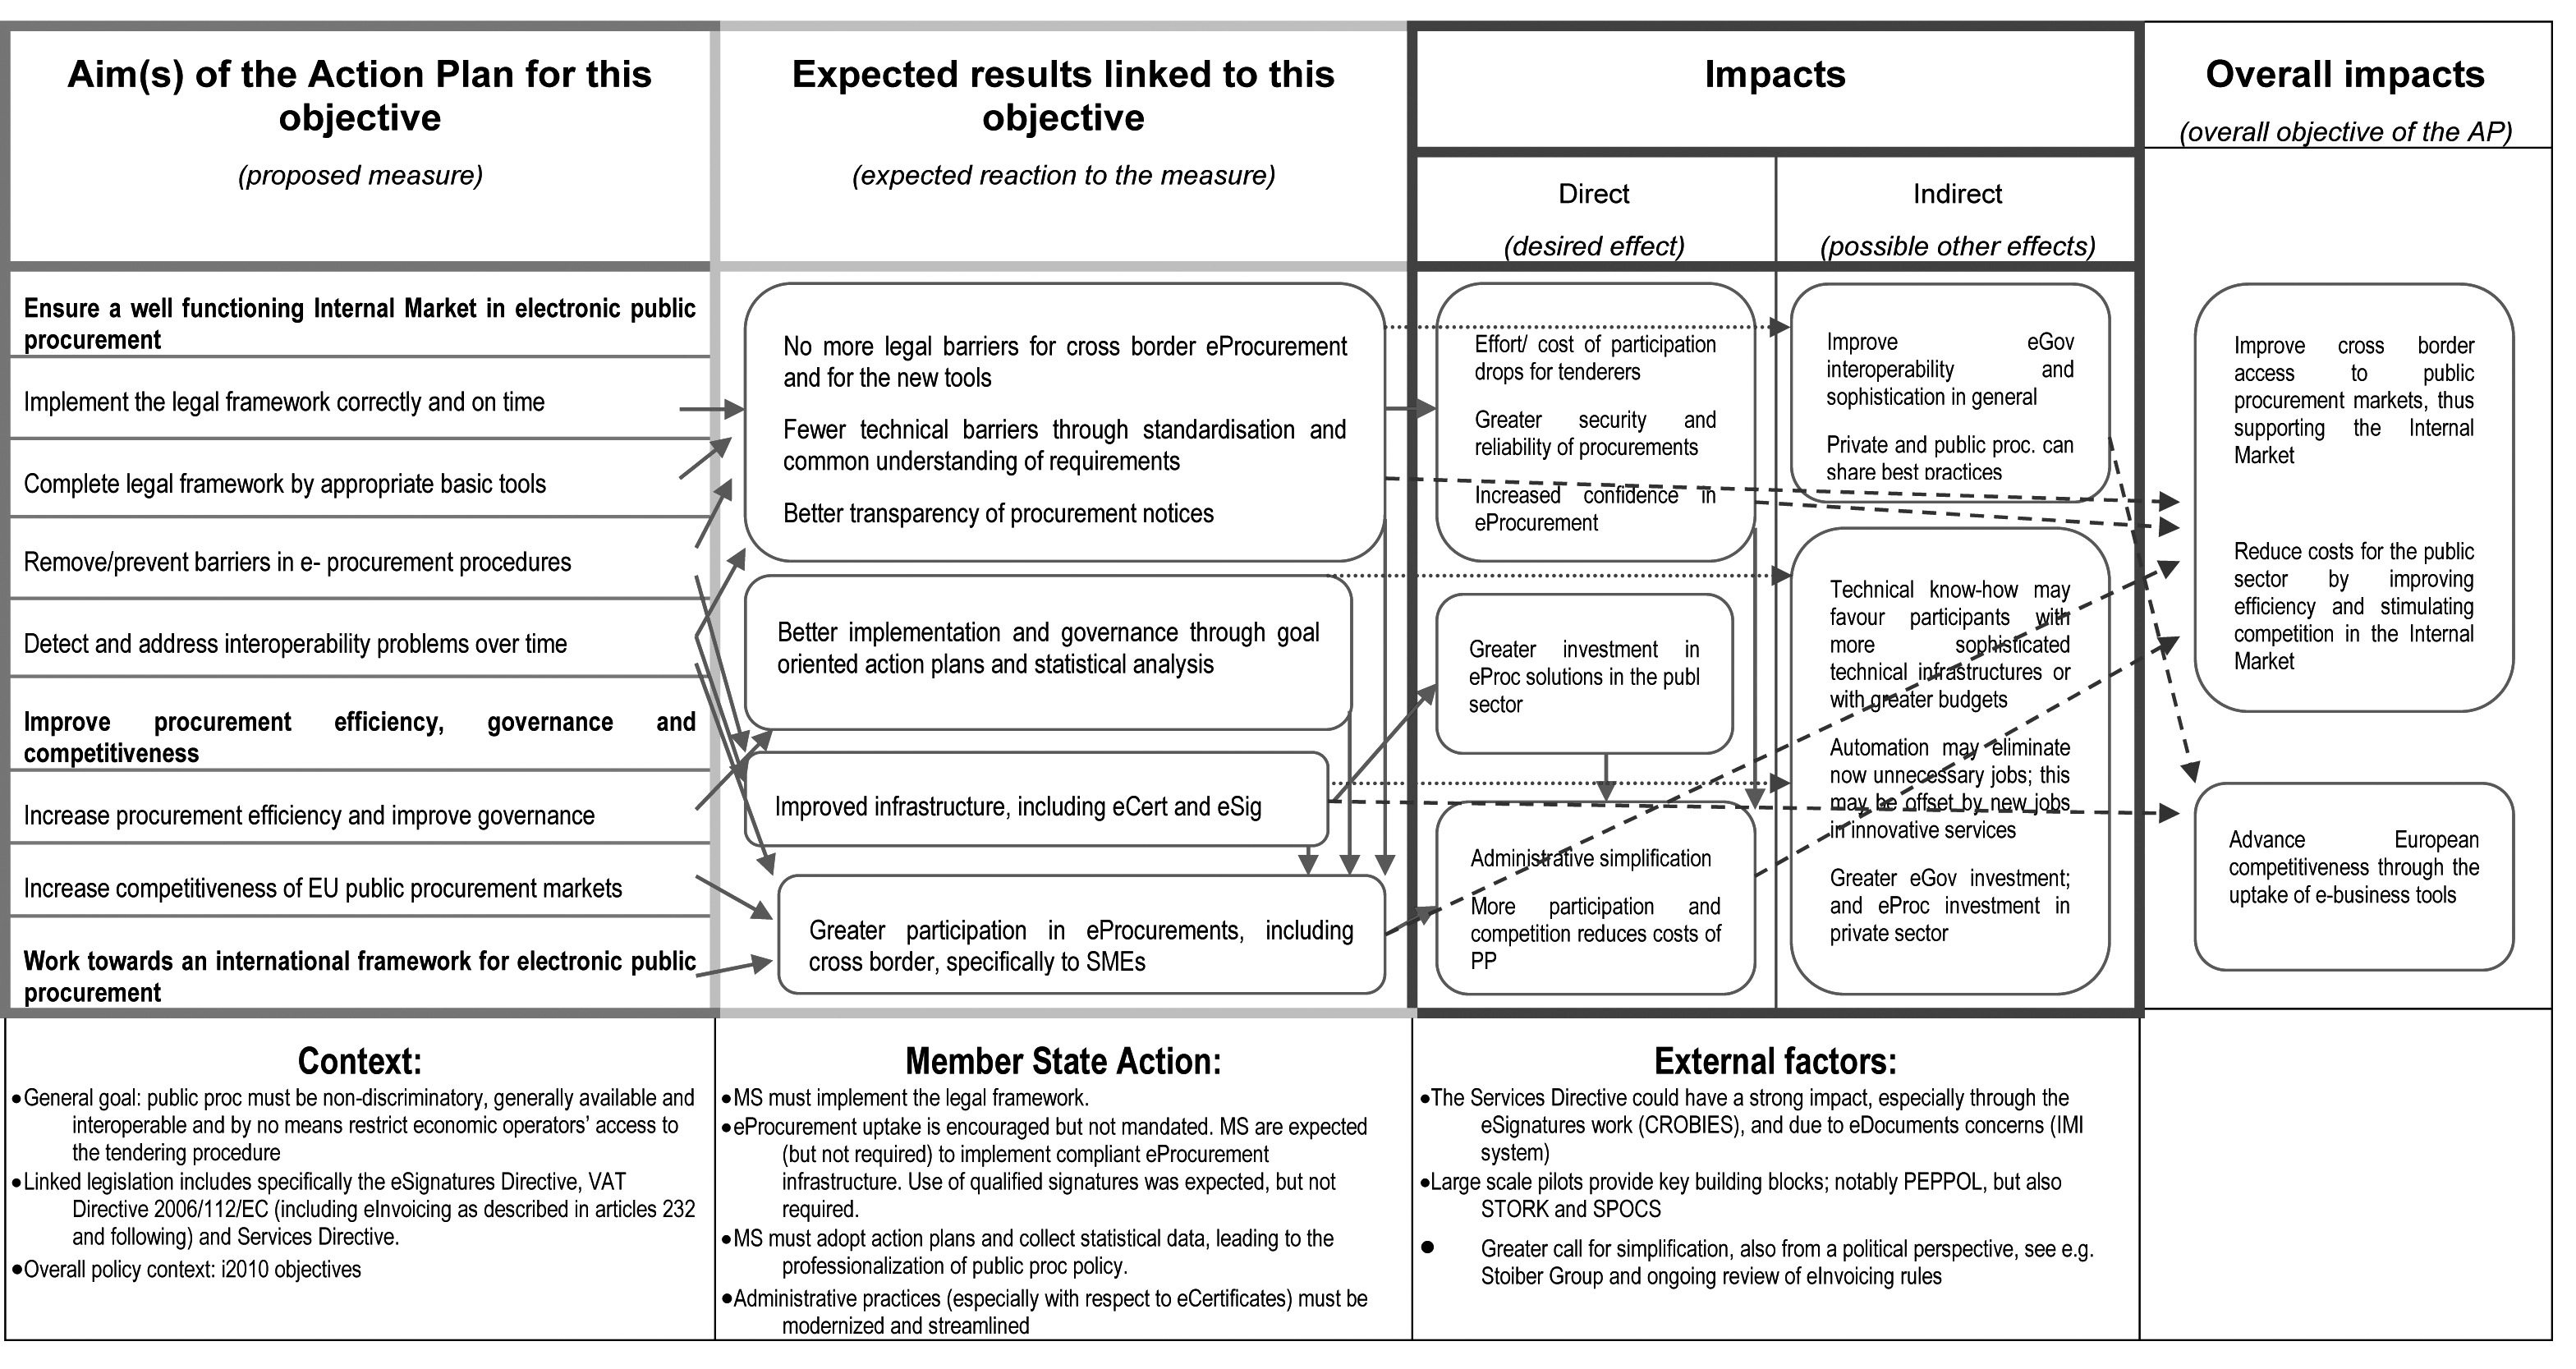
\includegraphics[width=16cm]{images/phd/eproc/ted-2}
\caption{Estrategia en e-Procurement de la Unión Europea elaborado por Siemens.}
\label{fig:ted-2}
\end{figure}

De igual forma, en este informe~\cite{siemensEval} se establecen una serie de métricas, ver Figura~\ref{fig:ted-3}, resultados e impacto, 
que deben servir como guía para las distintas acciones realizadas a nivel europeo y que
deben manifestarse en los distintos Estados Miembros.
% 
% 
\begin{figure}[!htb]
\centering
	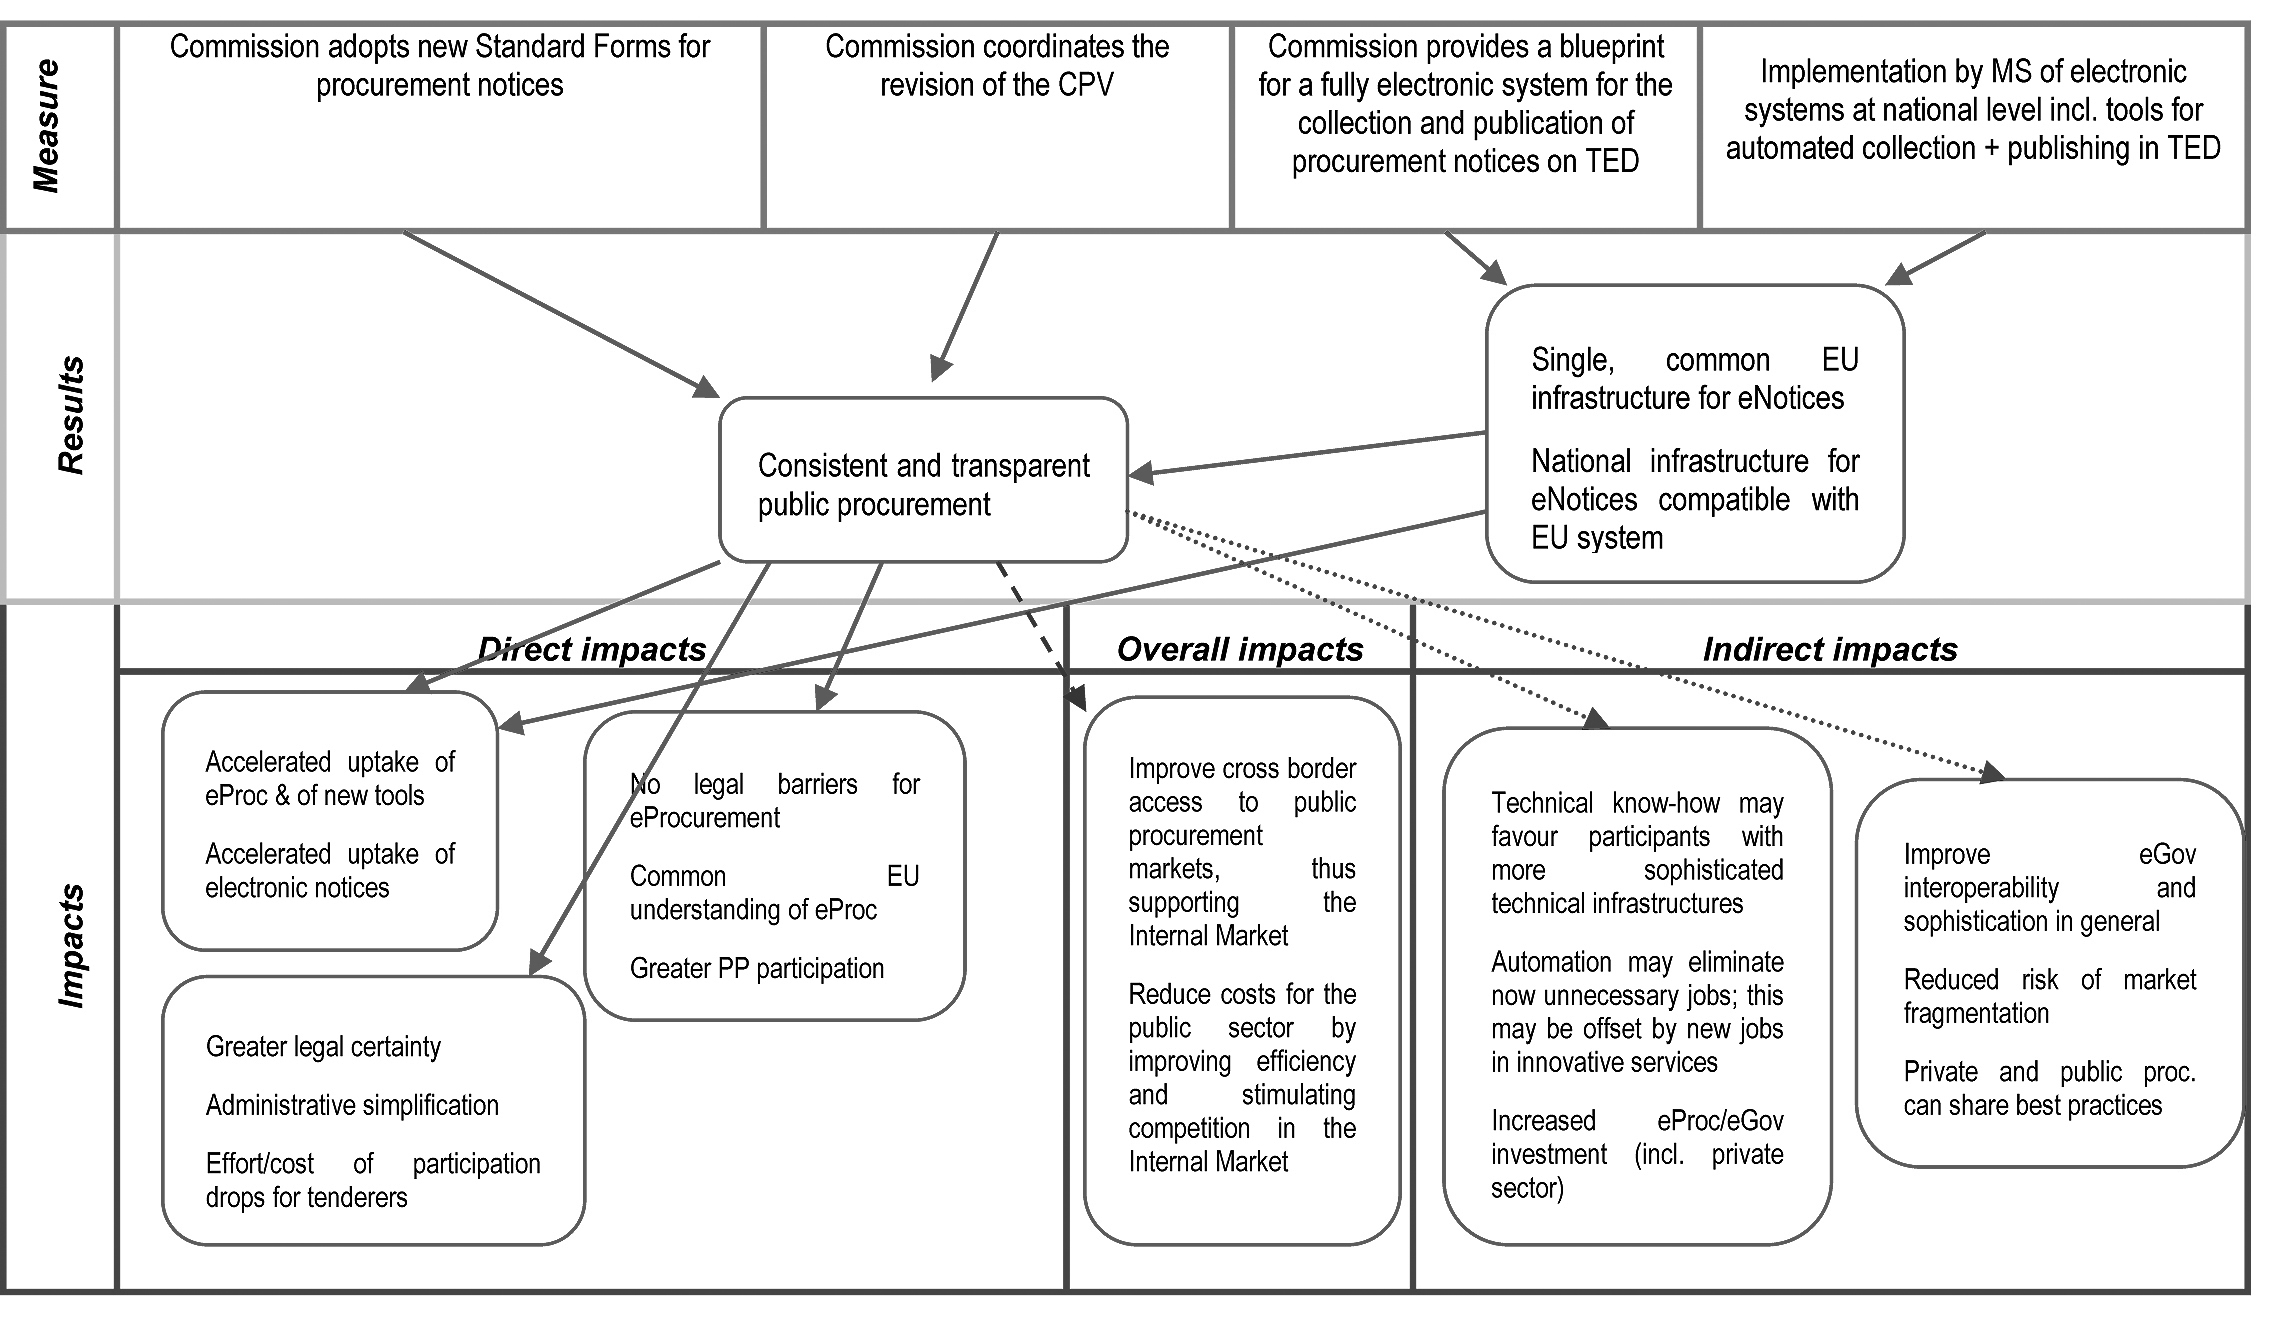
\includegraphics[width=16cm]{images/phd/eproc/ted-3}
\caption{Métricas en e-Procurement de la Unión Europea elaborado por Siemens.}
\label{fig:ted-3}
\end{figure}

A través del Plan de Acción de 2004 y de las posteriores evaluaciones continuas que se vienen realizando
en la Unión Europea, queda patente la importancia que desde las instituciones públicas se aplica
al proceso de contratación pública.

\subsection{Terminología}
Con el objetivo de favorecer la lectura del documento y disponer de una clara definición de cada uno
de los términos habitualmente utilizados en los procesos de contratación pública, se dispone a continuación
de una serie de definiciones (se incluyen las más importantes para el ámbito de este documento):

\begin{description}

\item [Adjudicatario (\textit{Successful tenderer}).] Empresa ganadora de un contrato público. Anteriormente en España
el proceso de adjudicación se dividía en provisional y definitivo. La diferenciación del procesos en dos partes, se 
establecía con el objetivo de comprobar si el adjudicatario cumplía las garantías necesarias.
Una vez que el proceso de selección previo se había superado, ya se establecía la formalización
del contrato con un determinado órgano y siguiendo la lista de candidatos que la Mesa de Contratación había valorado.

\item [Adjudicación (\textit{Awarding}).] Pasos que el órgano de contratación y los colectivos de soporte, 
comités de expertos o técnicos, siguen para decidir qué licitadores ofertan las mejores
opciones para ganar el contrato. Habitualmente, se utilizan diversas técnicas para
cada paso (técnica Delphi, entropía, etc.) aunque una de las máximas es obtener
la mejor relación oferta/precio, bajo las condiciones más óptimas.

\item [Agente externo.] Actor dentro del proceso de licitación que interviene en alguna
parte del proceso. Por ejemplo, en el ámbito español la Agencia Estatal de Administración Tributaria (\gls{AEAT}) o la
Tesorería General de la Seguridad Social (\gls{TGSS}), disponen de información susceptible de ser solicitada
por los sistemas de contratación electrónica de los órganos de contratación.

\item [Anuncio previo (\textit{Prior Information Notice}-\gls{PIN}).] Mensaje publicado por el órgano de contratación para informar sobre
la intención de contratar en un determinado período. Suelen contener información sobre
contratos de obras, suministros y servicios para los siguientes doce meses.

\item [Anuncio de adjudicación (\textit{Award notice}).] Mensaje publicado por el órgano de contratación mediante
los boletines oficiales como el ``Diario Oficial de la Unión Europea'' (\gls{DOUE}) y el ``Boletín
Oficial del Estado'' (\gls{BOE}), en los cuales se informa de los datos pertinentes de una
licitación y su adjudicatario. Suele corresponder a la información que se notifica
como resolución al proceso.

\item [Anuncio de licitación (\textit{Contract notice}).] Mensaje publicado por el órgano de contratación mediante
el cual se anuncia una nueva licitación, describiendo los términos legales, administrativos y
técnicos mínimos para que los empresarios expresen su interés de participación. La publicación
se realiza de forma oficial a través del \gls{DOUE}, \gls{BOE}, etc., y también forma parte del perfil
del comprador. En el ámbito español, existen otros tipos como el ``Anuncio Simplificado de Licitación'', utilizado 
en la fase de contratación específica de un Sistema Dinámico de Adquisición.

\item [Contrato (\textit{Contract}).] Documento de acuerdo entre un órgano de contratación y un licitador, que 
establece las condiciones de contratación de acuerdo los pliegos publicados por el primero
y la oferta realizado por el segundo. Incluye firmas de las partes contratantes y toda la información
pertinente. Este documento representa la culminación del acto de licitación.

\item [Empresario (\textit{Economic operator}).] Es el ``operador económico'' que designa tanto a un ``contratista''
como a un ``proveedor'' o ``prestador de servicios''. Otros términos que se utilizan
para especificar esta figura son ``Licitador'' o ``Adjudicatario''.

\item [Espacio de trabajo de la licitación.] Espacio digital en el cual se registra toda
la documentación y artefactos relativos al proceso administrativo. Es el expediente electrónico
del proceso, que puede ser implementado mediante carpetas virtuales, registros, repositorios, etc.

\item [Licitar (\textit{Call for tenders} o \textit{tendering}).] En su acepción más amplia: acto por el cual el Estado concede contratos para la
ejecución de servicios, suministros y obras de interés público; la adjudicación definitiva de
dichos contratos puede ir precedida de un concurso o subasta en la que varias personas, físicas
o jurídicas, presentan sus cotizaciones o los precios que cobrarían por la ejecución del
contrato. También se denomina al subconjunto de tareas ejecutadas por el empresario,
en interacción con el Órgano de contratación, destinadas a presentar una Oferta en respuesta
a un Anuncio de Licitación o a una invitación a oferta.

\item [Oferta (\textit{tender}).] Documento que un empresario envía a
un órgano de contratación para licitar.

\item [Órgano de contratación (\textit{Contracting authority}).] Organizaciones, departamentos, secciones
o colegiados con la capacidad legal y estatutaria para celebrar
contratos en nombre de las entidades públicas.

\item [Perfil del contratante (\textit{Buyer profile}).] Página web en la cual se publicita toda la información
referente a los contratos de un determinado órgano de contratación.

\item [Plataforma de contratación (\textit{e-Procurement System}).] Plataforma electrónica a través de la cual se gestiona
el proceso administrativo de la contratación electrónica.

\item [Otros.] A continuación se disponen de algunos términos habitualmente utilizados
en la bibliografía relativa a contratación pública y que se consideran de interés:
acuerdo de exclusión, acuerdo marco (\textit{framework agreement}), 
agencia de garantía (\textit{guarrantee agency}), agencia registradora (\textit{registration agency}), 
artefacto (\textit{artifact}), agente externo (\textit{external agent}),
claúsulas administrativas, comité de expertos (\textit{technical committee}), 
diálogo competitivo (competitive dialogue), expediente (\textit{procurement File}), 
garantía definitiva (\textit{tender guarantee}), invitación, mesa de contratación,
oferta indicativa, oferta temeraria, pliegos (\textit{tender information}), prescripciones técnicas,
procedimiento (\textit{procedure}): abierto, negociado, restringido, Registro Oficial de Licitadores y de Empresas Clasificadas (\gls{ROLEC} en el ámbito español), sistema dinámico de adquisición 
(\textit{dynamic purchasing system}), etc.
\end{description}

\section{Contratación Pública}
En general los participantes en un proceso de contratación pública, no difieren de la ejecución
de cualquier contrato habitual salvo que uno de los actores, como parte contratante sea la Administración Pública, 
mientras que por la parte contratada pueden distinguirse tanto a personas físicas como jurídicas con capacidad de obrar y con solvencia acreditada tanto
a nivel económico-financiero como técnico.

La Administración se estructura en diferentes órganos, compuestos por distintas unidades organizativas o 
agentes responsables de llevar a cabo las actividades de los procesos administrativos y entre ellos
el proceso de contratación pública. Para estudiar los actores participantes en el proceso de contratación, se pueden seguir diferentes criterios pero por sencillez se suele utilizar una distribución funcional
según las actividades a desarrollar por cada uno de ellos. A continuación, comentaremos algunos de estos
agentes haciendo referencias a la situación actual en el ámbito de la Administración General del Estado
en España.

\begin{description}
 \item [Contratación.] Son las entidades con capacidad para obrar un contrato. Normalmente,
se agrupan bajo el término ``Órganos de Contratación'' y dependen de la propia estructura y organización
de la Administración. Dependiendo de distintas variables como el tipo de contrato, el importe del 
mismo o el lugar de celebración, los órganos cambiarán de acuerdo a su potestad. Como ejemplo y siguiendo
la estructura y organización de la Administración General del Estado, se establecen distintas unidades
organizativas que tendrán capacidad de actuar como Órganos de Contratación. En este caso y siguiendo 
la Ley 6/1997~\cite{l6-1997}, de 14 de abril de Organización y Funcionamiento de la Administración 
General del Estado, la cual en su exposición de motivos, refiere a uno de los preceptos fundamentales
que la Constitución Española de 1978 dedica en su artículo 103 a la actividad de la Administración, así, objetividad,
generalidad, eficacia, jerarquía, descentralización, desconcentración y coordinación se constituyen como principios básicos 
de funcionamiento de la Administración.

Esta misma ley, en su artículo 3, establece que la organización y actuación de la Administración General del Estado se realizará de acuerdo 
con respeto al principio de legalidad y de acuerdo a los siguientes principios (entre otros):
\begin{itemize}
 \item De organización:
\begin{itemize}
 \item Jerarquía.
 \item Descentralización funcional.
 \item Desconcentración funcional y territorial
 \item Economía, suficiencia y adecuación estricta de los medios a los fines institucionales.
 \item Coordinación.
\end{itemize}
 \item De funcionamiento: 
\begin{itemize}
\item Eficacia en el cumplimiento de los objetivos fijados.
\item Eficiencia en la asignación y utilización de los recursos públicos
\item Programación y desarrollo de objetivos y control de la gestión y de los resultados.
\item Responsabilidad por la gestión pública.
\item Racionalización y agilidad de los procedimientos administrativos y de las actividades de gestión
\item Servicio efectivo a los ciudadanos.
\item Objetividad y transparencia de la actuación administrativa.
\end{itemize}
\end{itemize} 

También y como ejemplo, en el Capítulo II de dicha ley se establece
la ``Organización Administrativa'', tanto de la Administración General del Estado como de sus Organismos públicos. La Administración 
General del Estado responde a una organización funcional en Departamentos ministeriales y de gestión
territorial integrada en Delegaciones de Gobierno en las propias
Comunidades Autónomas. La organización de la Administración Central distingue
entre órganos superiores (S) y órganos directivos (D):
\begin{itemize}
 \item Ministros. (S)
 \item Secretarios de Estado. (S)
 \item Subsecretarios y Secretarios generales. (D)
 \item Secretarios generales técnicos y Directores generales. (D)
 \item Subdirectores generales. (D)
\end{itemize}

Esta estructuración administrativa resulta idónea para exponer una distribución modelo que dependiendo de cada
caso puede variar: Comisión Europea, Universidad, etc., pero que sin embargo contribuye a crear una noción de
cómo una ordenación administrativa con sus distintos órganos que cuentan con capacidad de actuar como órganos contratantes.

\item [Gestión.] Contribuyen al proceso de contratación pública, dando el apoyo a las actividades
de ejecución de las tareas económico-administrativas para tramitar el proceso. En general, suelen formar
parte del propio Órgano de Contratación, aunque también pueden tener carácter general, como por ejemplo la 
Dirección General del Tesoro y Política Financiera siendo los encargados en última instancia de realizar el pago
de los importes de los contratos.

\item [Control.] Se encargan de asegurar la legalidad de los procesos de contratación. En el ámbito
de la Administración General del Estado, se podría destacar la Intervención General de la Administración del Estado y el
Tribunal de Cuentas.

\item [Asesoría.] Especialistas colaboradores de la contratación para diferentes aspectos: jurídicos, técnicos, económicos u 
otros que pudieran requerirse. Siguiendo con el ejemplo anterior, y en general: la Junta Consultiva de Contratación Administrativa o 
los Servicios Jurídicos del Estado, por otra parte, en particular podríamos citar: las Oficinas Técnicas de Supervisión
de Proyectos o la Comisión Interministerial de Adquisición de Bienes y Servicios Informáticos (CIABSI).


\item [Publicidad.] Canales de comunicación para hacer públicas las convocatorias y los procedimientos de contratación. En el 
ámbito de la Administración General del Estado podemos citar el BOE o la Plataforma
de Contratación del Estado. En el ámbito europeo hay que mencionar el DOUE, \textit{Tenders Electronic Daily} (\gls{TED}) 
o el Sistema de Información para la contratación pública europea (SIMAP).


\item [Otros.] Funciones de carácter transversal, como las obligaciones tributarias o de seguridad social. Continuando con el ejemplo citado, 
la Agencia Tributaria o la Tesorería de la Seguridad Social serían agentes participantes que dan soporte a las actividades derivadas de la contratación pública.
\end{description}


\subsection{Ejemplo: la Administración General del Estado en España}
En esta sección se recoge parte de la casuística implicada en un proceso de contratación
pública con la Administración General del Estado, con el objetivo de mostrar las actividades
que se han de desarrollar y desvelando algunas de las interacciones que surgen entre los distintos
agentes con las consiguientes necesidades de interoperabilidad e integración.

Actualmente cada Comunidad Autónoma tiene su propia plataforma de contratación y perfil
del contratante, ver Tabla~\ref{table:plataformas}, en la cual se pueden realizar las operaciones del proceso de contratación pública 
electrónica. En muchos de los casos están enlazadas con la Plataforma de Contratación del Estado~\cite{PlataformaContratacionEstado}
y siguen sus estándares como ``Componentes y Documentos Interoperables para la Contratación Electrónica'' (\gls{CODICE}) 
para la gestión de la información y documentación generada a lo largo del proceso. Evidentemente y dependiendo de 
la capacidad de cada órgano de contratación podrán desplegar su propia plataforma, la administración en España sigue un modelo
descentralizado y coordinado desde la Administración General del Estado, o bien utilizar la infraestructura común.
%Comunidad, Plataforma

\begin{longtable}[c]{|p{7cm}|p{8cm}|} 
\hline
  \textbf{Comunidad Autónoma} & \textbf{Plataforma de Contratación} \\\hline
\endhead
Andalucía & \url{http://www.juntadeandalucia.es/contratacion} \\ \hline
Aragón & \url{http://portal.aragon.es/portal/page/portal/CPUBLICA#} \\ \hline
Castilla y León & \url{http://www.jcyl.es/web/jcyl/Portada/es/Plantilla100/1246947706077/_/_/_} \\ \hline
Castilla La Mancha & \url{http://pagina.jccm.es/contratacion/} \\ \hline
Cantabria  & \url{https://aplicaciones5.cantabria.es/PerfilContratante} \\ \hline
Canarias & \url{http://www.gobcan.es/perfildelcontratante/contenido} \\ \hline
Cataluña & \url{https://contractaciopublica.gencat.cat} \\ \hline
Región de Murcia & \url{http://www.carm.es/web/pagina?IDCONTENIDO=6427&IDTIPO=100} \\ \hline
Comunidad de Madrid & \url{http://www.madrid.org/cs/Satellite?cid=1203334374251&language=es&pagename=PortalContratacion/Page/PCON_contenidoFinal} \\ \hline
Comunidad Valenciana & \url{https://www.contratacion.gva.es/WebContrataP} \\ \hline
Cdad. Foral de Navarra & \url{http://www.navarra.es/home_es/Servicios/Portal+contrataciones/} \\ \hline
Extremadura & \url{https://contratacion.juntaextremadura.net} \\ \hline
Galicia & \url{http://www.contratosdegalicia.es/} \\ \hline
Illes Balears & \url{http://www.plataformadecontractacio.caib.es/} \\ \hline
La Rioja & \url{http://www.larioja.org/npRioja/default/defaultpage.jsp?idtab=26275} \\ \hline
Principado de Asturias & \url{https://sede.asturias.es} \\ \hline
País Vasco & \url{http://www.euskadi.net/r33-2288/es/contenidos/informacion/perfil_anuncios/} \\ \hline
 \hline
\caption{Plataformas de Contratación en las Comunidades Autónomas.}\label{table:plataformas}\\    
\end{longtable}

En estas plataformas las operaciones a realizar, los idiomas disponibles, etc., son variados, si además se amplia el rango
de órganos de contratación a Universidades, Ayuntamientos, Parroquias Rurales, Mancomunidades, etc.,  y ahora se proyecta
a nivel europeo es factible advertir la diversificación y la replicación de esfuerzos que se están efectuando en este ámbito. 
Por ello, iniciativas como la Plataforma de Contratación del Estado o \gls{TED} ayudan a unificar y facilitar el acceso a las distintas fases del proceso
de contratación pública.

\section{Contratación Pública Electrónica: e-Procurement}
El término \gls{e-Procurement}~\cite{Podlogar2007} se utiliza para designar el uso de medios y tecnologías electrónicos para llevar a cabo
las operaciones y comunicaciones relacionadas con la contratación pública, y en general para todos aquellos procesos~\cite{DBLP:journals/tcci/Alor-HernandezAJPRMBG10}
en los que participen proveedores y consumidores de un cierto servicio o producto. En el caso particular de las Administraciones
Públicas se utiliza esta terminología para definir las operaciones llevadas a cabo para adquirir bienes o servicios mediante
distintos métodos: contratación directa, centrales de contratación, contratos de urgencia y emergencia, etc.

La importancia del proceso de contratación pública electrónica, va más allá de la simple transición del papel ya que puede
aportar mejoras relevantes en eficiencia de las adquisiciones, gestión global del proceso de contratación pública y en general, 
al funcionamiento de los mercados de las administraciones.

La tendencia actual para acelerar la implantación de procesos de contratación, se alinea con las directrices de impulso de la administración
electrónica como camino para la transformación del funcionamiento de la administración pública y la prestación de servicios. En este sentido,
la Agenda Digital de la Comisión Europea está trabajando en una guía o ``libro blanco'', para fijar las medidas que aseguren el despliegue
de una infraestructura integradora de la contratación pública que atender las necesidades de los distintos países. Como primer paso para la 
consecución de este gran objetivo, se ha elaborado una declaración de intenciones a través de un ``libro verde'' en el cual se pone de manifiesto el ambicioso objetivo
de uso de las TICs en este dominio de la administración pública. 

El nacimiento de esta propuesta está fechada en el año 2005 cuando los Ministros de la Unión Europea manifestaron su deseo de conseguir ``en el año 2010,
que como mínimo el $50$\%  de toda la contratación pública que rebase el umbral de contratación pública de la Unión \gls{Europea} se lleve a cabo
por medios electrónicos''. Teniendo presente esta intención se modificó la legislación pertinente y se puso en práctica el ``Plan 
de Acción sobre Contratación Electrónica''~\cite{plan2004} en el año 2004. Aunque desde un punto de vista teórico se han sentado las bases para la contratación
pública electrónica, la realidad es que el grado de implantación efectiva es muy inferior al esperado, ya que la complejidad subyacente,
ver Figura~\ref{fig:e-proc-complexity}, abarca distintos niveles: técnico, logístico y administrativo. Siguiendo la evaluación realizada por la Comisión, se señala que al
menos el $5\%$ del presupuesto total destinado a la contratación en los \gls{Estados} Miembros que iniciaron esta línea de acción se adjudica
por canales electrónicos.

\begin{figure}[!htb]
\centering
	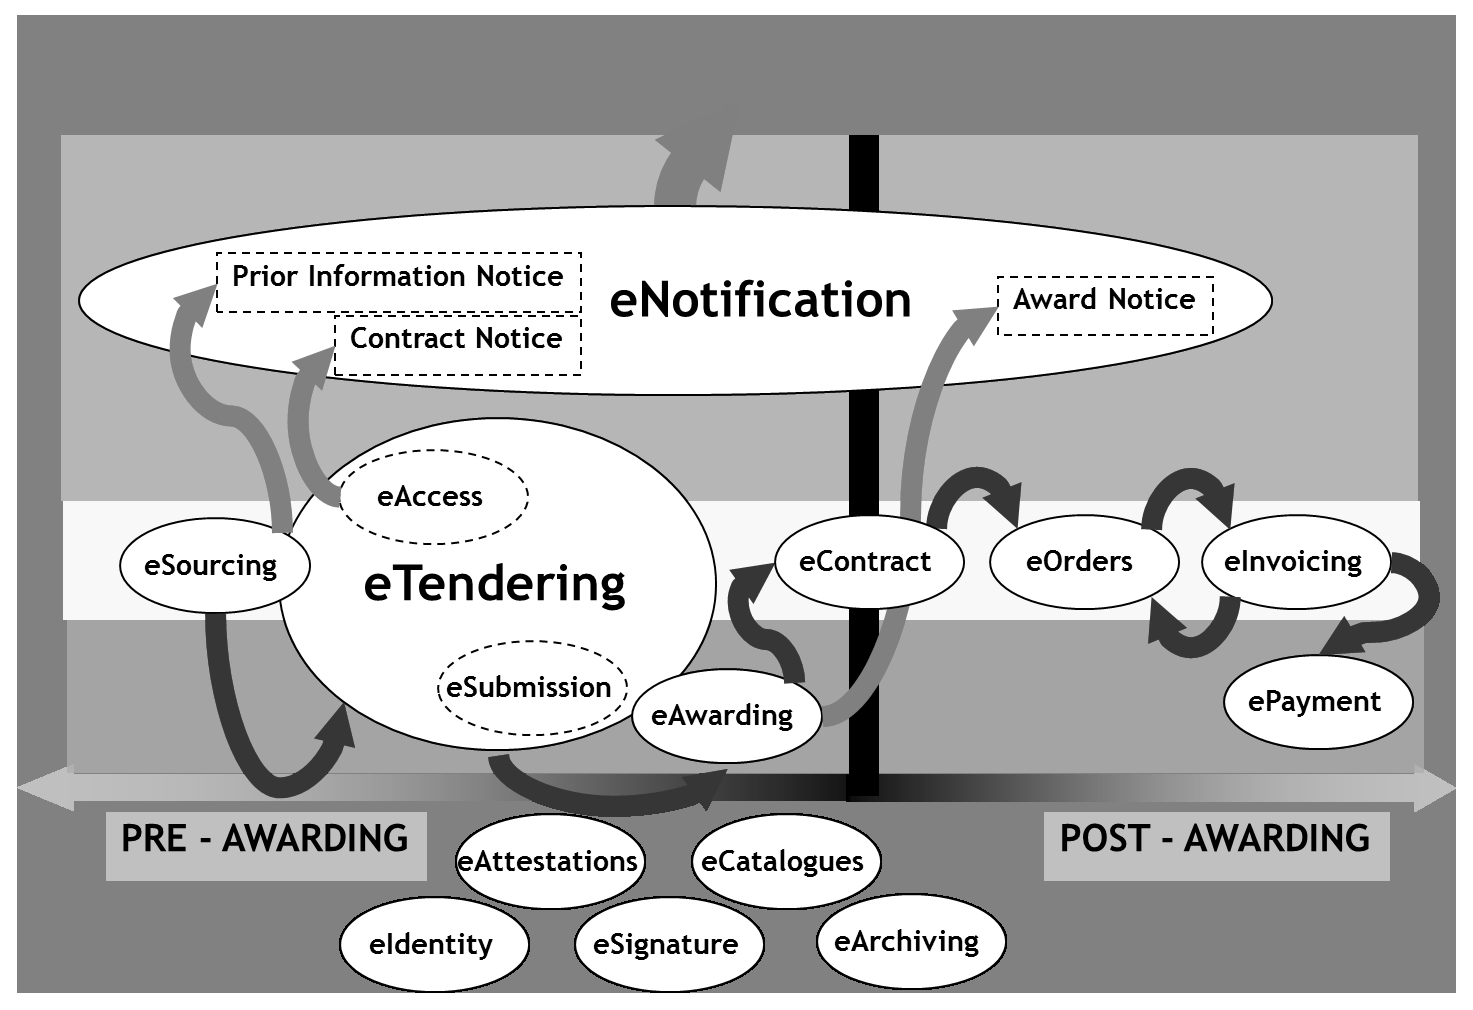
\includegraphics[width=16cm]{images/phd/eproc/e-proc-complexity}
\caption{Diagrama de Complejidad y Fases de e-Procurement por la Unión Europea.}
\label{fig:e-proc-complexity}
\end{figure}

Ahora bien, el crecimiento de este porcentaje depende en buena medida de que la contratación electrónica sea implantada a todos los niveles
administrativos (local, regional y estatal), para ello se debe contar con la tecnología necesaria, en muchos casos ya disponible, así como
de plataformas de contratación que se puedan integrar a nivel operativo para que el tráfico a través de las mismas genere la masa
crítica suficiente como para alcanzar los requisitos fijados por la Comisión para lograr la innovación en este proceso. Además de incrementar el uso
de medios electrónicos en la contratación pública, surge la oportunidad de armonizar este proceso administrativo de forma transfronteriza
de tal forma que se impulse la participación de las empresas en procesos de contratación pública más allá de su región de origen, fomentando 
así la competitividad y mejorando tanto los productos como los servicios a contratar y por extensión potenciando tanto las posibilidades
de las entidades dispuestas a licitar, como los servicios prestados por la propia administración.


\subsection{Definición de Contratación Electrónica}
Siguiendo la definición realizada por la Unión Europea~\cite{e-Proc-green-paper}, se puede definir contratación electrónica como:

\textit{La contratación electrónica es un término general utilizado para designar la sustitución de los
procedimientos basados en soporte de papel por el tratamiento y la comunicación mediante
TIC a lo largo de toda la cadena de contratación pública. Supone la introducción de
procedimientos electrónicos para sustentar las distintas fases del proceso de contratación, es
decir, publicación de los anuncios de licitación, suministro del pliego de condiciones,
presentación de ofertas, evaluación, adjudicación, pedido, facturación y pago.}

\textit{Los procedimientos vinculados a la facturación y el pago (posteriores a la adjudicación) no
son específicos de la contratación; por tanto, es posible aplicar en el ámbito de la contratación
pública electrónica soluciones desarrolladas para un mercado más amplio (de empresa a
empresa) 6 . No obstante, en algunas fases (notificación, presentación de propuestas,
valoración y pedido) se requieren soluciones específicas. Las fases de presentación,
valoración y pedido son las más arduas ya que exigen la aplicación de una serie de protocolos
y normas consensuados para organizar el intercambio de documentos complejos, así como la
interacción entre el comprador público y los proveedores.}

No obstante, consultando la actividad propuesta por la Unión Europea para la contratación electrónica
se han fijado algunos aspectos que deberán todavía co-existir de forma no automatizada. Es el caso
de la documentación de procesos de contratación complejos como pueden ser los planos y diseños
de obras, ya que es necesario disponer de los originales de forma impresa y normalizados para poder ser consultados por
los propios expertos de la administración y realizar las validaciones pertinentes. 

Ahora bien para dar cabida a la contratación pública electrónica se ha necesitado un esfuerzo por parte
de las diferentes Administraciones para la creación de portales en los cuales contener los anuncios de licitación y facilitar
el acceso a la descripción de los mismos, y más en particular a los pliegos de condiciones técnicas y económicas. 
De esta forma, se da un paso hacia delante al disponer de un servicio público electrónico de ``principio a fin''. 
Este tipo de plataformas han sido denominadas como ``plataformas de contratación electrónica'', como ejemplo
podemos citar la ``Plataforma de Contratación del Estado''~\cite{PlataformaContratacionEstado} entre otras. 
También y de forma obligatoria, aquellos entes que quieran hacer uso de la contratación pública electrónica deben 
publicar su ``Perfil de Contratante''~\cite{PerfilContratante}. En el caso de España, existen otras características que impulsarán la 
contratación pública electrónica como la factura electrónica~\cite{FacturaElectronica}.

Por otra parte, el proceso de contratación pública y en concreto el que concierne a la contratación pública electrónica cuenta
con distintas fases con diferentes objetivos y que se deben abordar en un contexto común, definiendo
para cada uno de ellos sus características. A continuación, se disponen de las distintas fases
identificadas~\cite{siemensEval}, ver Figura~\ref{fig:ted-1}, por la Comisión en este ámbito y que sirven para focalizar el objetivo de este documento.


\begin{figure}[!htb]
\centering
	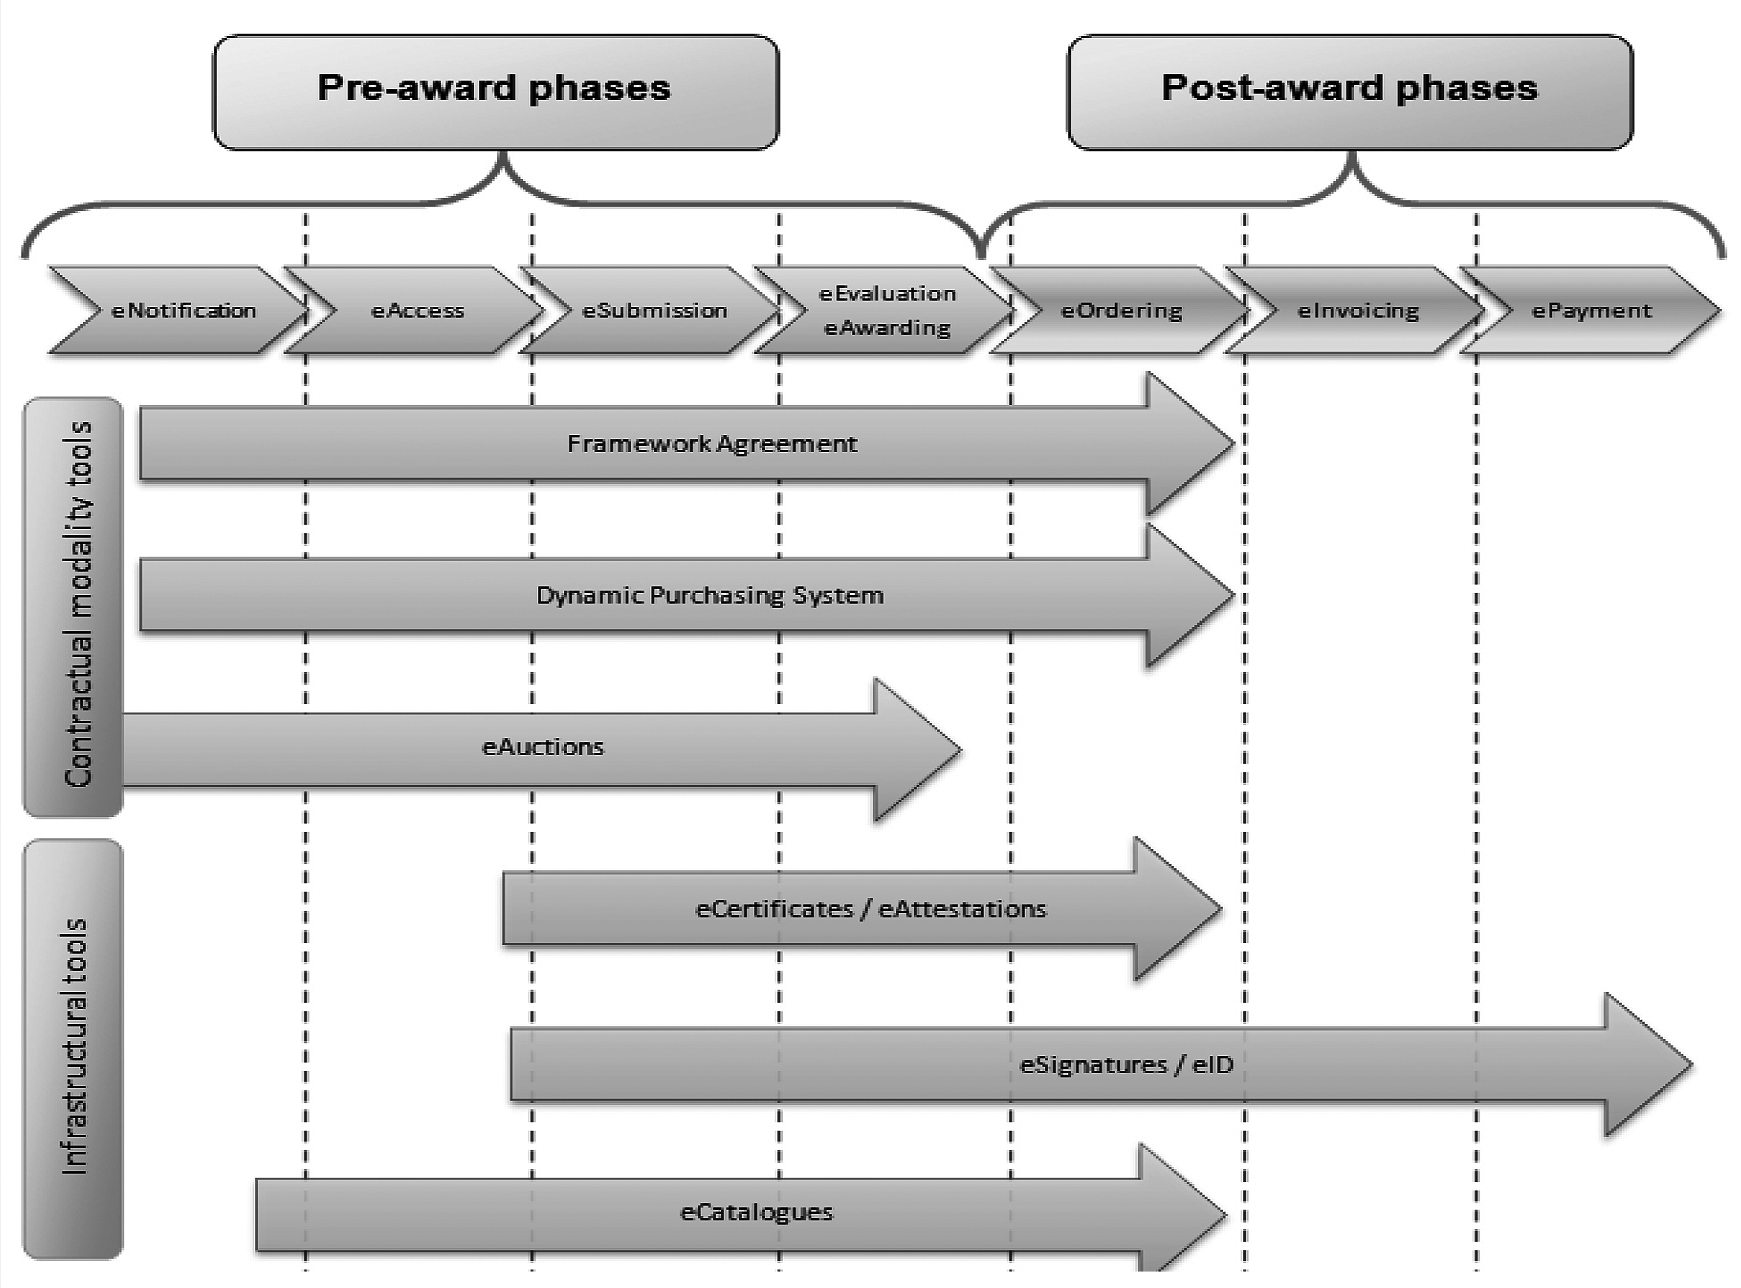
\includegraphics[width=16cm]{images/phd/eproc/ted-1}
\caption{Fases de e-Procurement definidas por la Comisión Europea.}
\label{fig:ted-1}
\end{figure}


\begin{description}

 \item [\textit{eNotification}.] Esta fase cubre la publicación de anuncios de licitación. Se trata
de un proceso unilateral que conlleva la comunicación entre órgano de contratación y el sistema
de publicación. Es el primer paso para facilitar el acceso a la información contenida
en los anuncios de licitación. El principal desafío de esta fase es realizar la publicación
de la información de la forma más estandarizada posible. Actualmente, se utiliza XML como 
formato de publicación y mediante herramientas como eSenders es posible enviar la información
a través de distintos canales como fax o correo electrónico. Los órganos de contratación 
se encargan de esta tarea buscando agilizar el proceso de publicación y asegurando
que no existan errores. A nivel europeo, en el año 2009, alrededor del $89\%$ de los anuncios de licitación
utilizan un medio electrónico para ser publicados. En la Figura~\ref{fig:circa-1}, se puede ver el uso 
de los medios para la publicación de anuncios realizados por los distintos Estados Miembros de forma agregada. Por ejemplo y comparando algunos países, 
en Noruega sería el $100\%$ (ver Figura~\ref{fig:circa-7}), España un $88,8\%$  (ver Figura~\ref{fig:circa-6}) , Alemania un $82,9\%$ 
(ver Figura~\ref{fig:circa-5}) y Turquía un $50\%$ (ver Figura~\ref{fig:circa-8}).


\begin{figure}[!htb]
\centering
	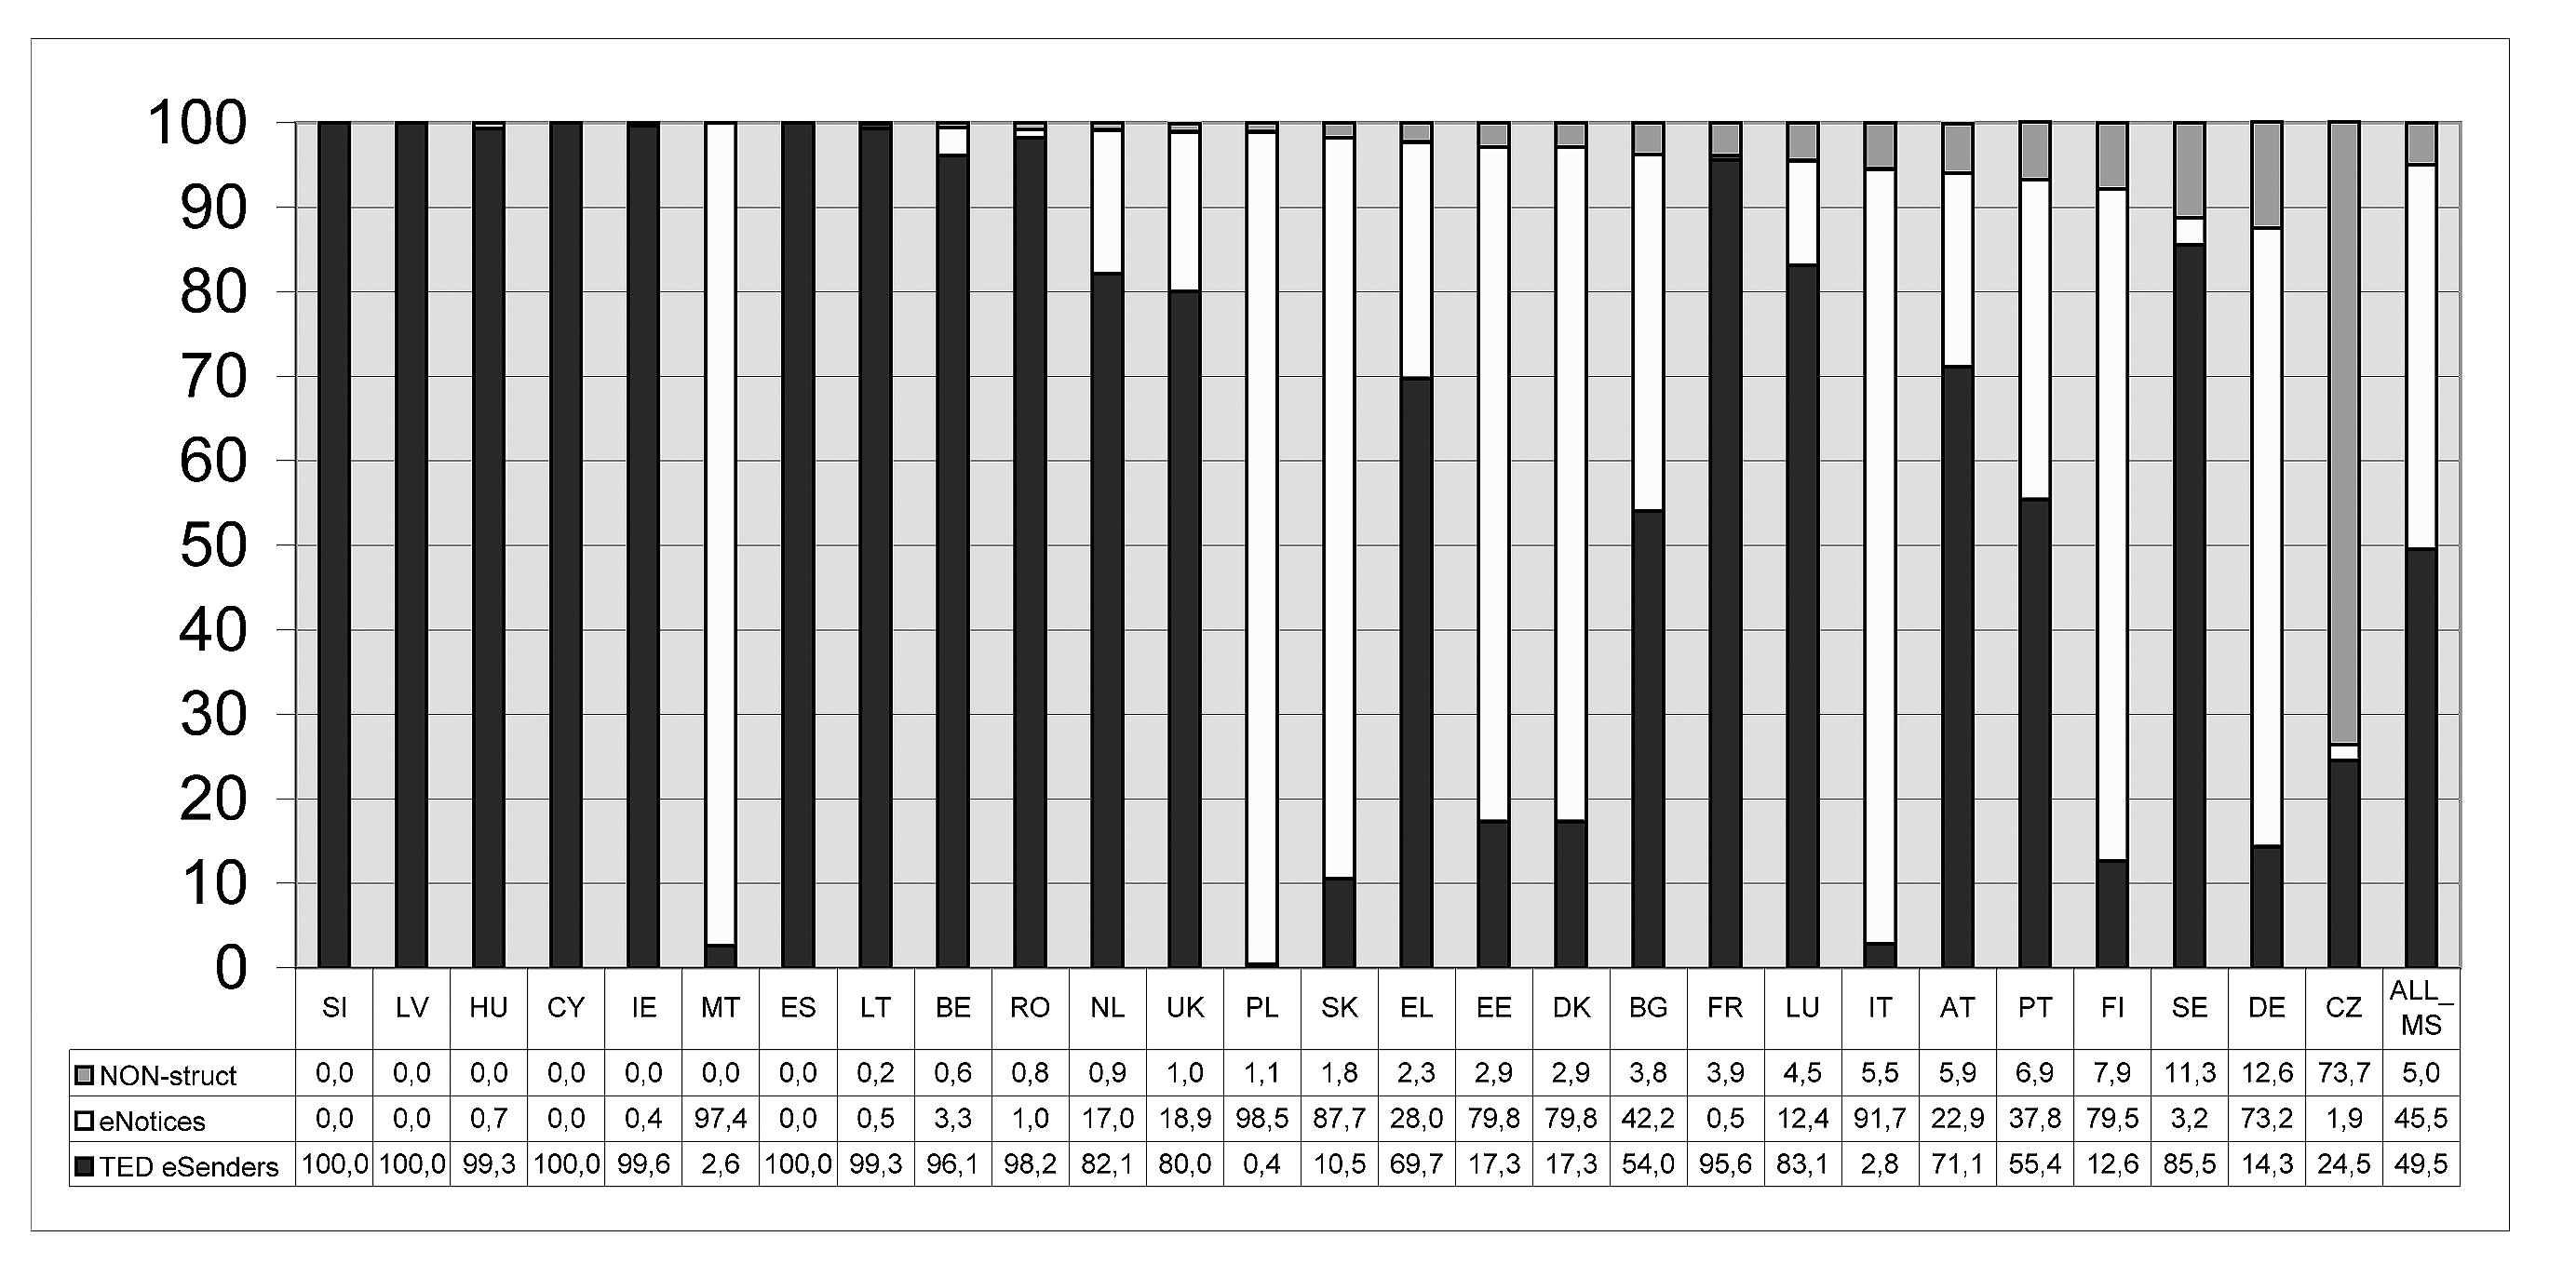
\includegraphics[width=16cm]{images/phd/eproc/circa-1}
\caption{Porcentaje y Tipo de Publicación de Anuncios de Licitación en TED.}
\label{fig:circa-1}
\end{figure}


\begin{figure}[!htb]
\centering
	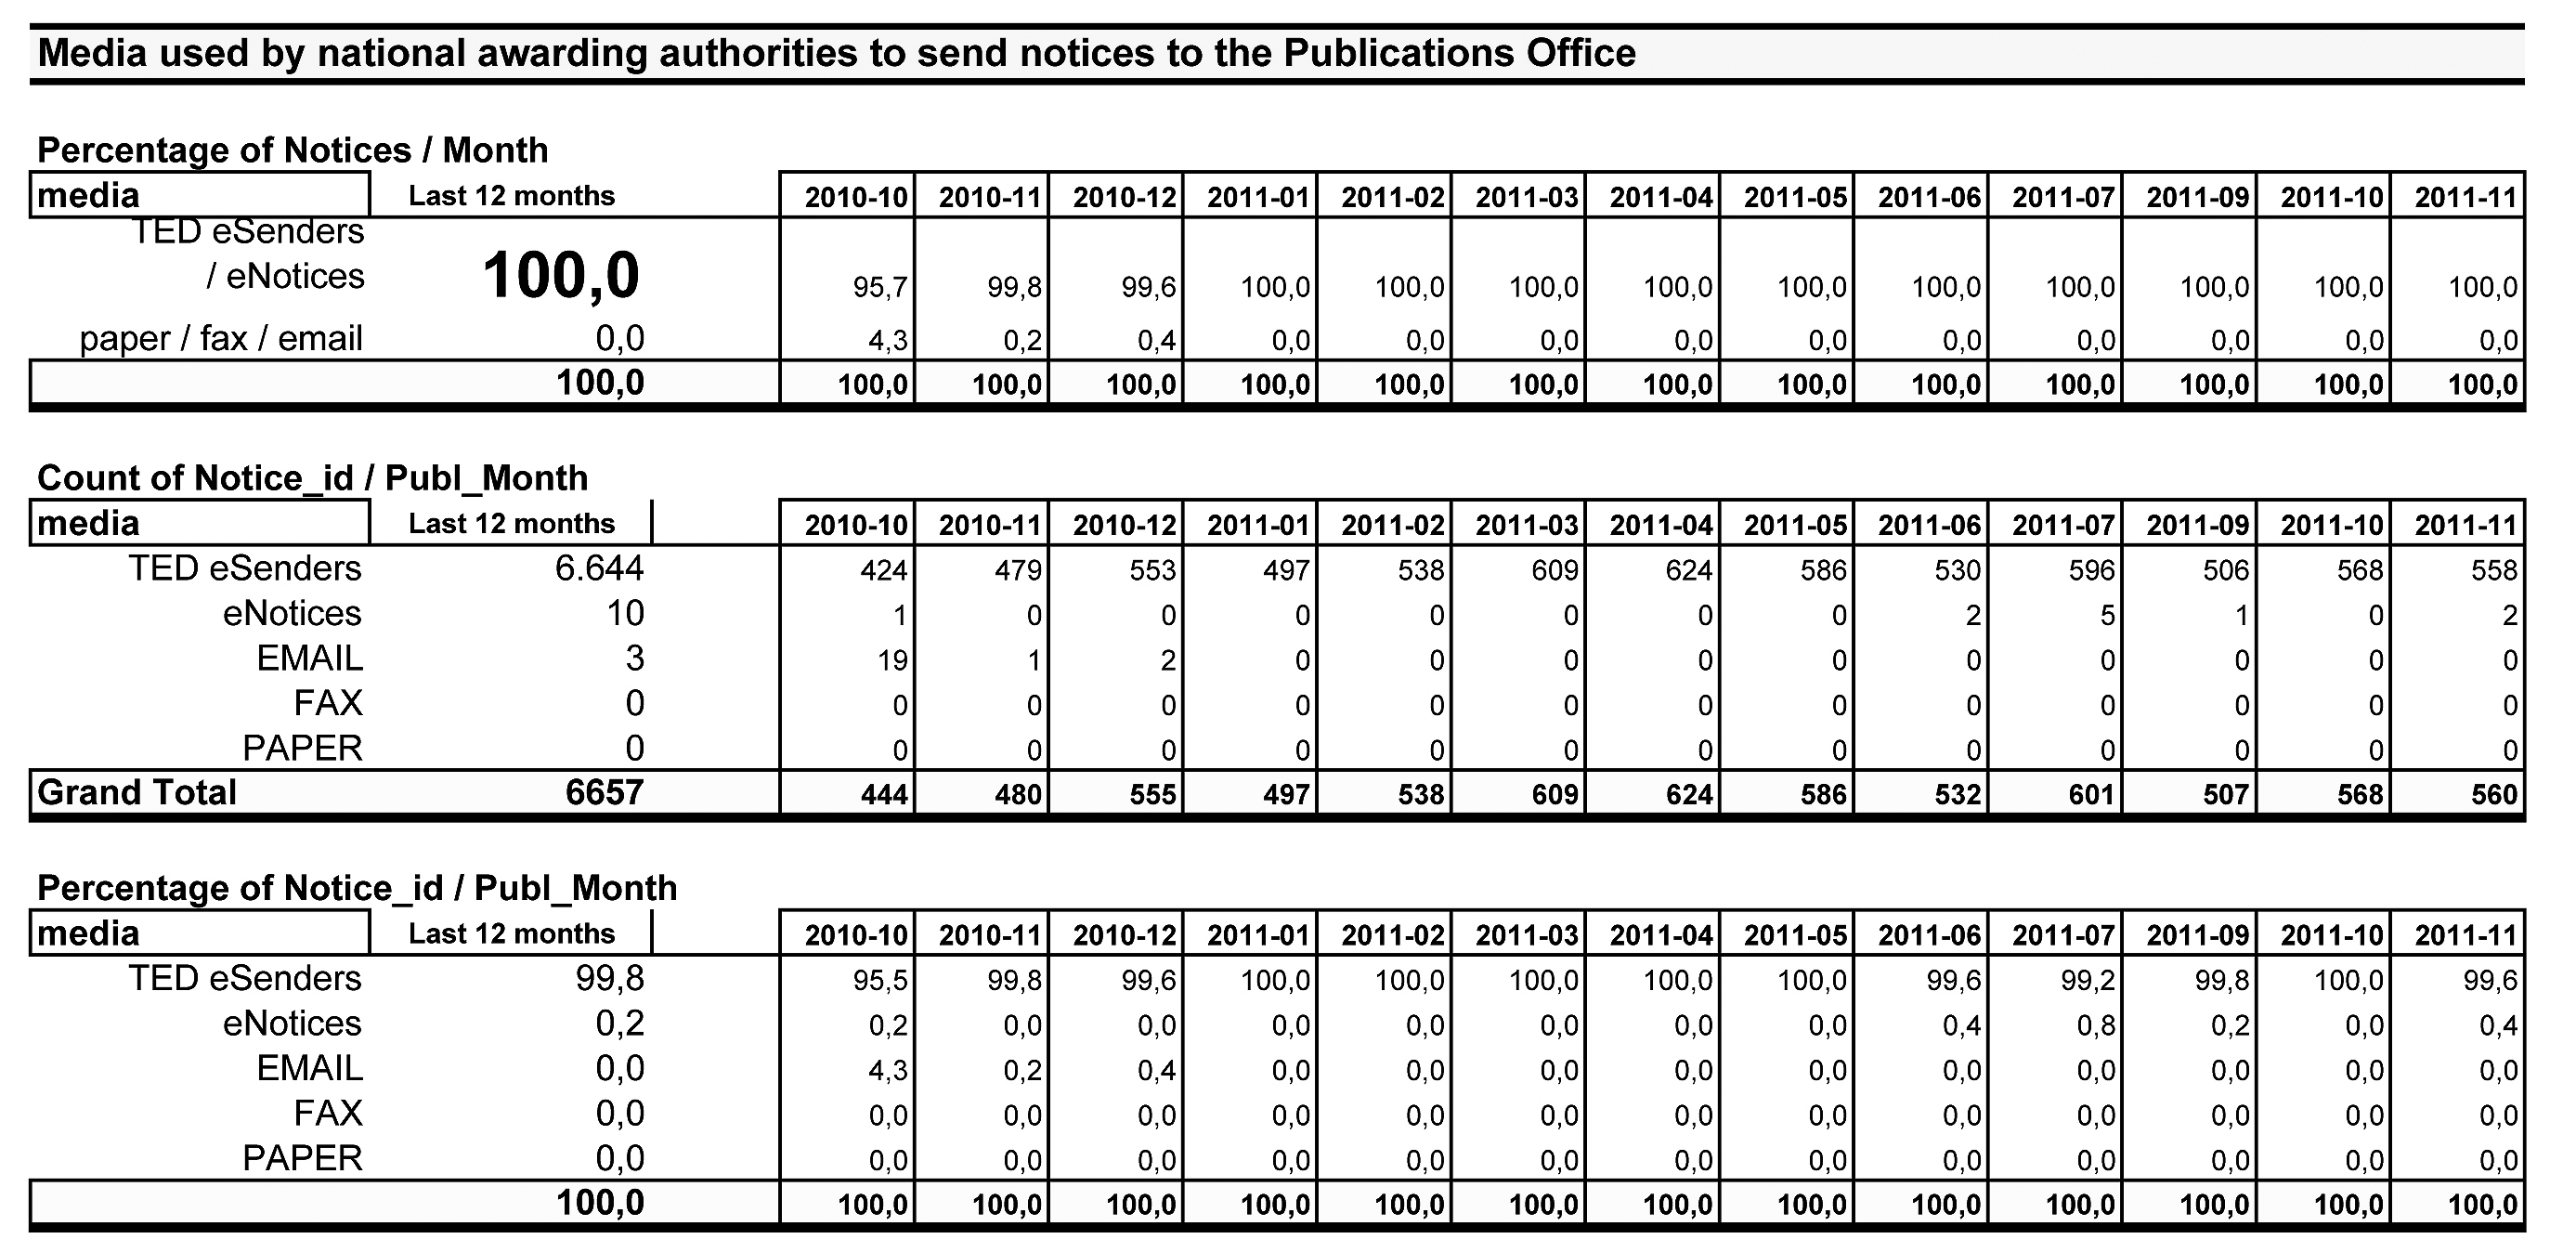
\includegraphics[width=16cm]{images/phd/eproc/circa-7}
\caption{Porcentaje y Tipo de Publicación de Anuncios de Licitación en TED de Noruega.}
\label{fig:circa-7}
\end{figure}


\begin{figure}[!htb]
\centering
	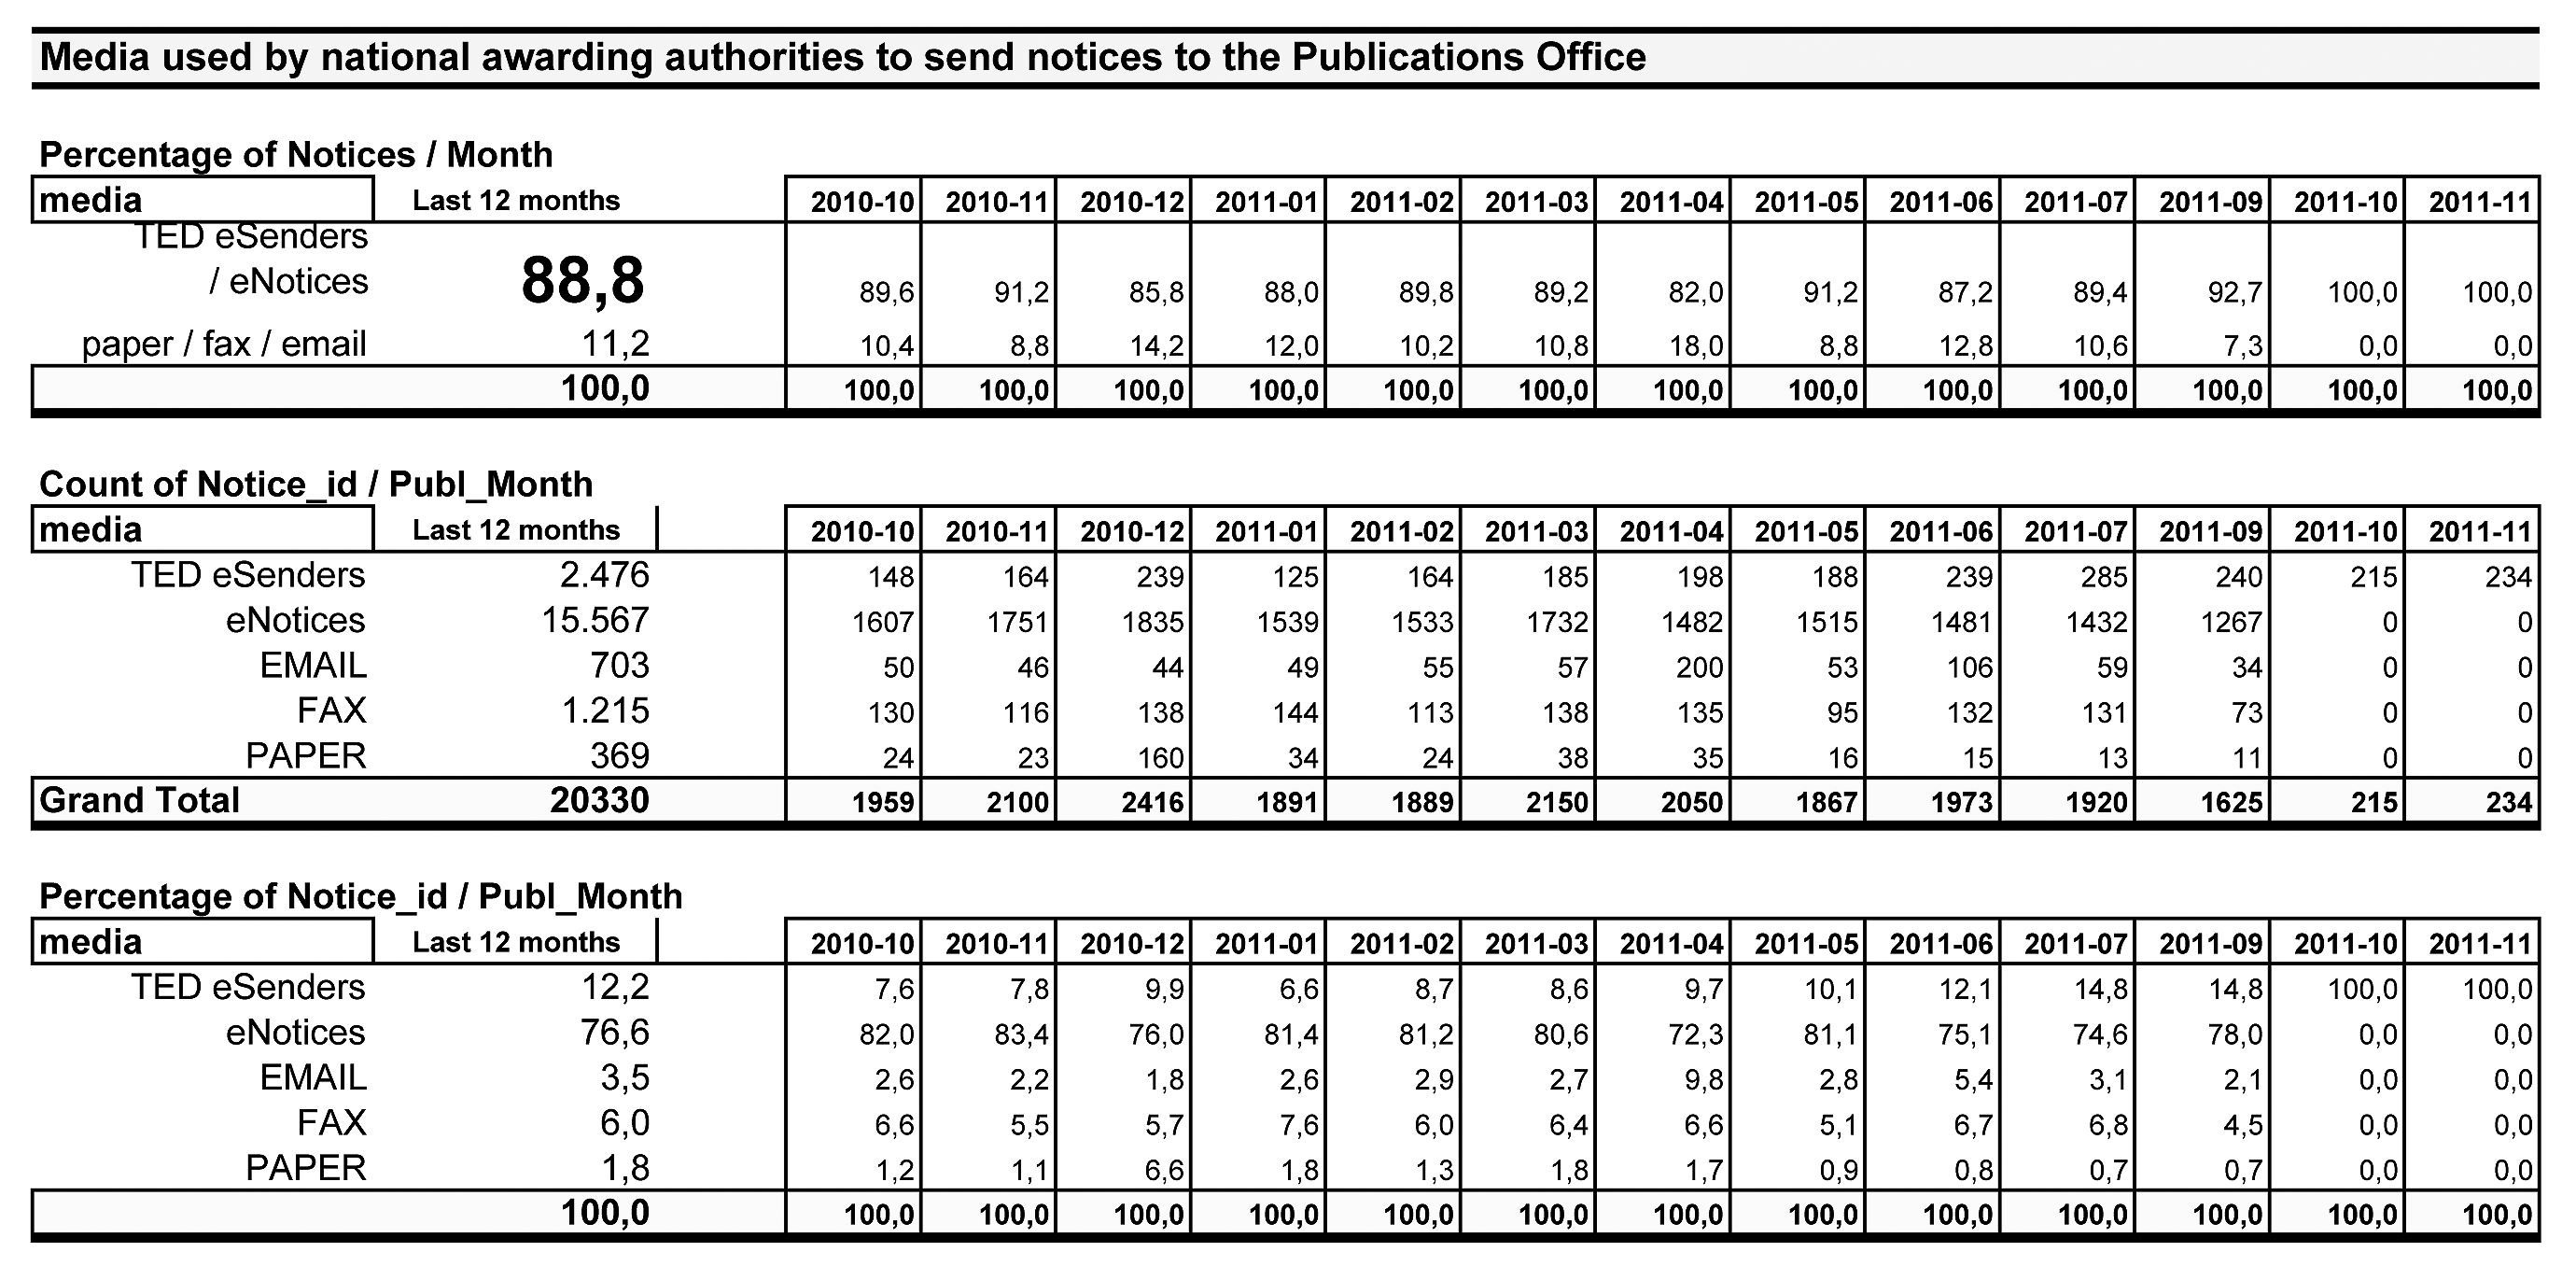
\includegraphics[width=16cm]{images/phd/eproc/circa-6}
\caption{Porcentaje y Tipo de Publicación de Anuncios de Licitación en TED de España.}
\label{fig:circa-6}
\end{figure}



 \begin{figure}[!htb]
\centering
	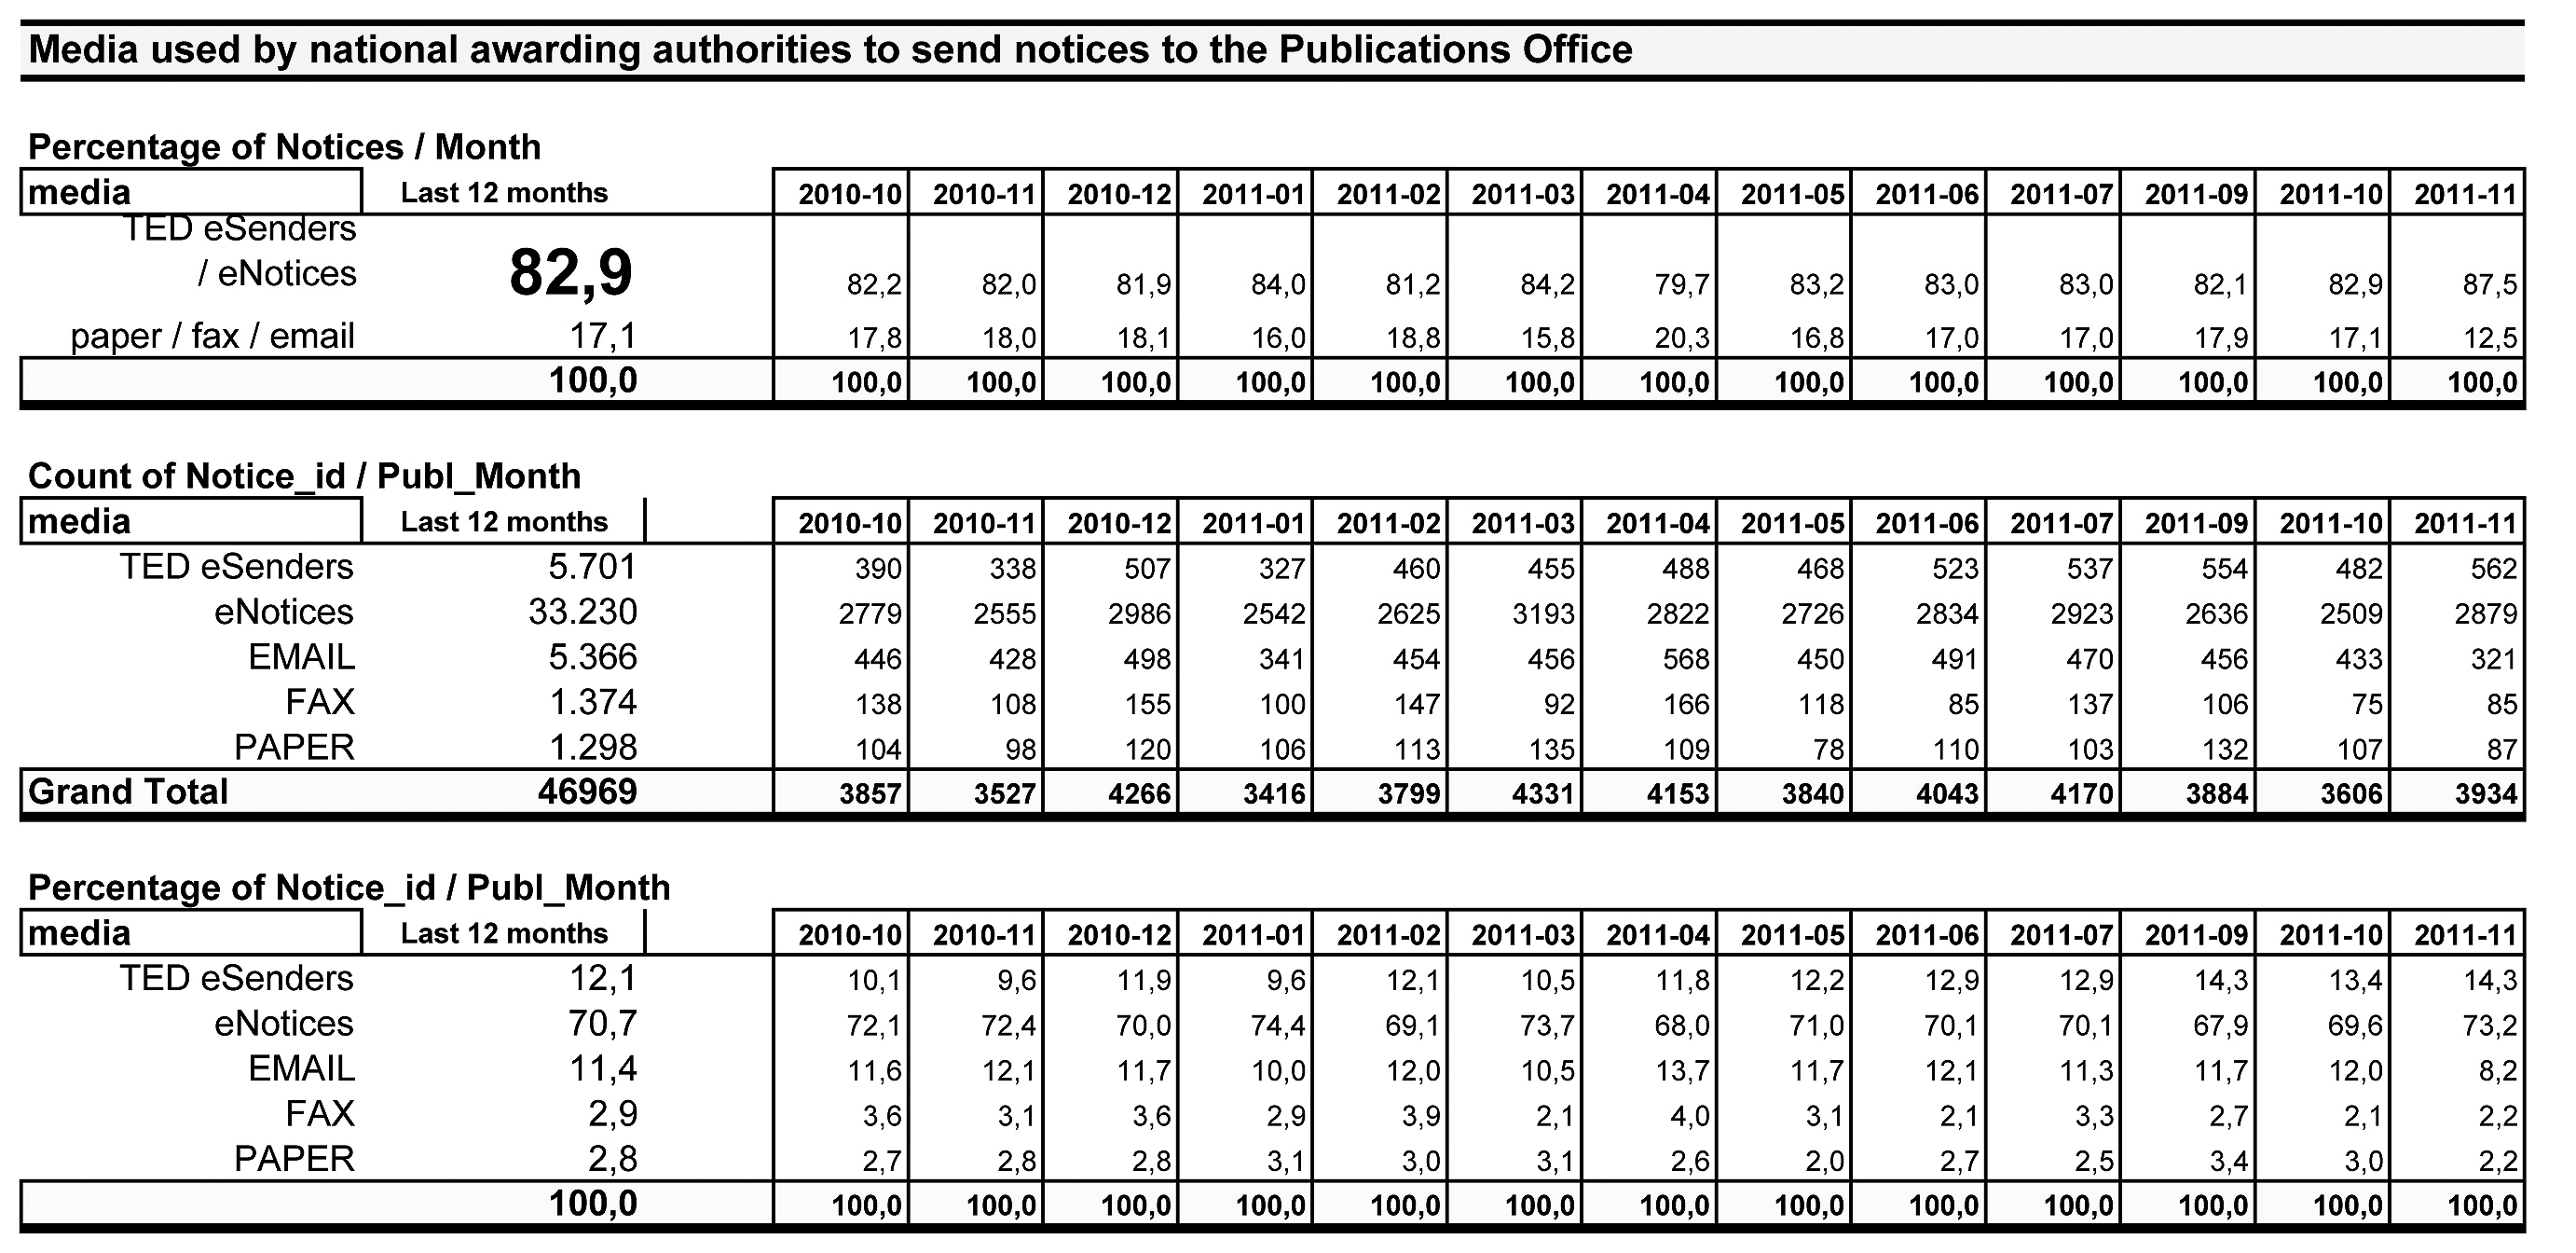
\includegraphics[width=16cm]{images/phd/eproc/circa-5}
\caption{Porcentaje y Tipo de Publicación de Anuncios de Licitación en TED de Alemania.}
\label{fig:circa-5}
\end{figure}



\begin{figure}[!htb]
\centering
	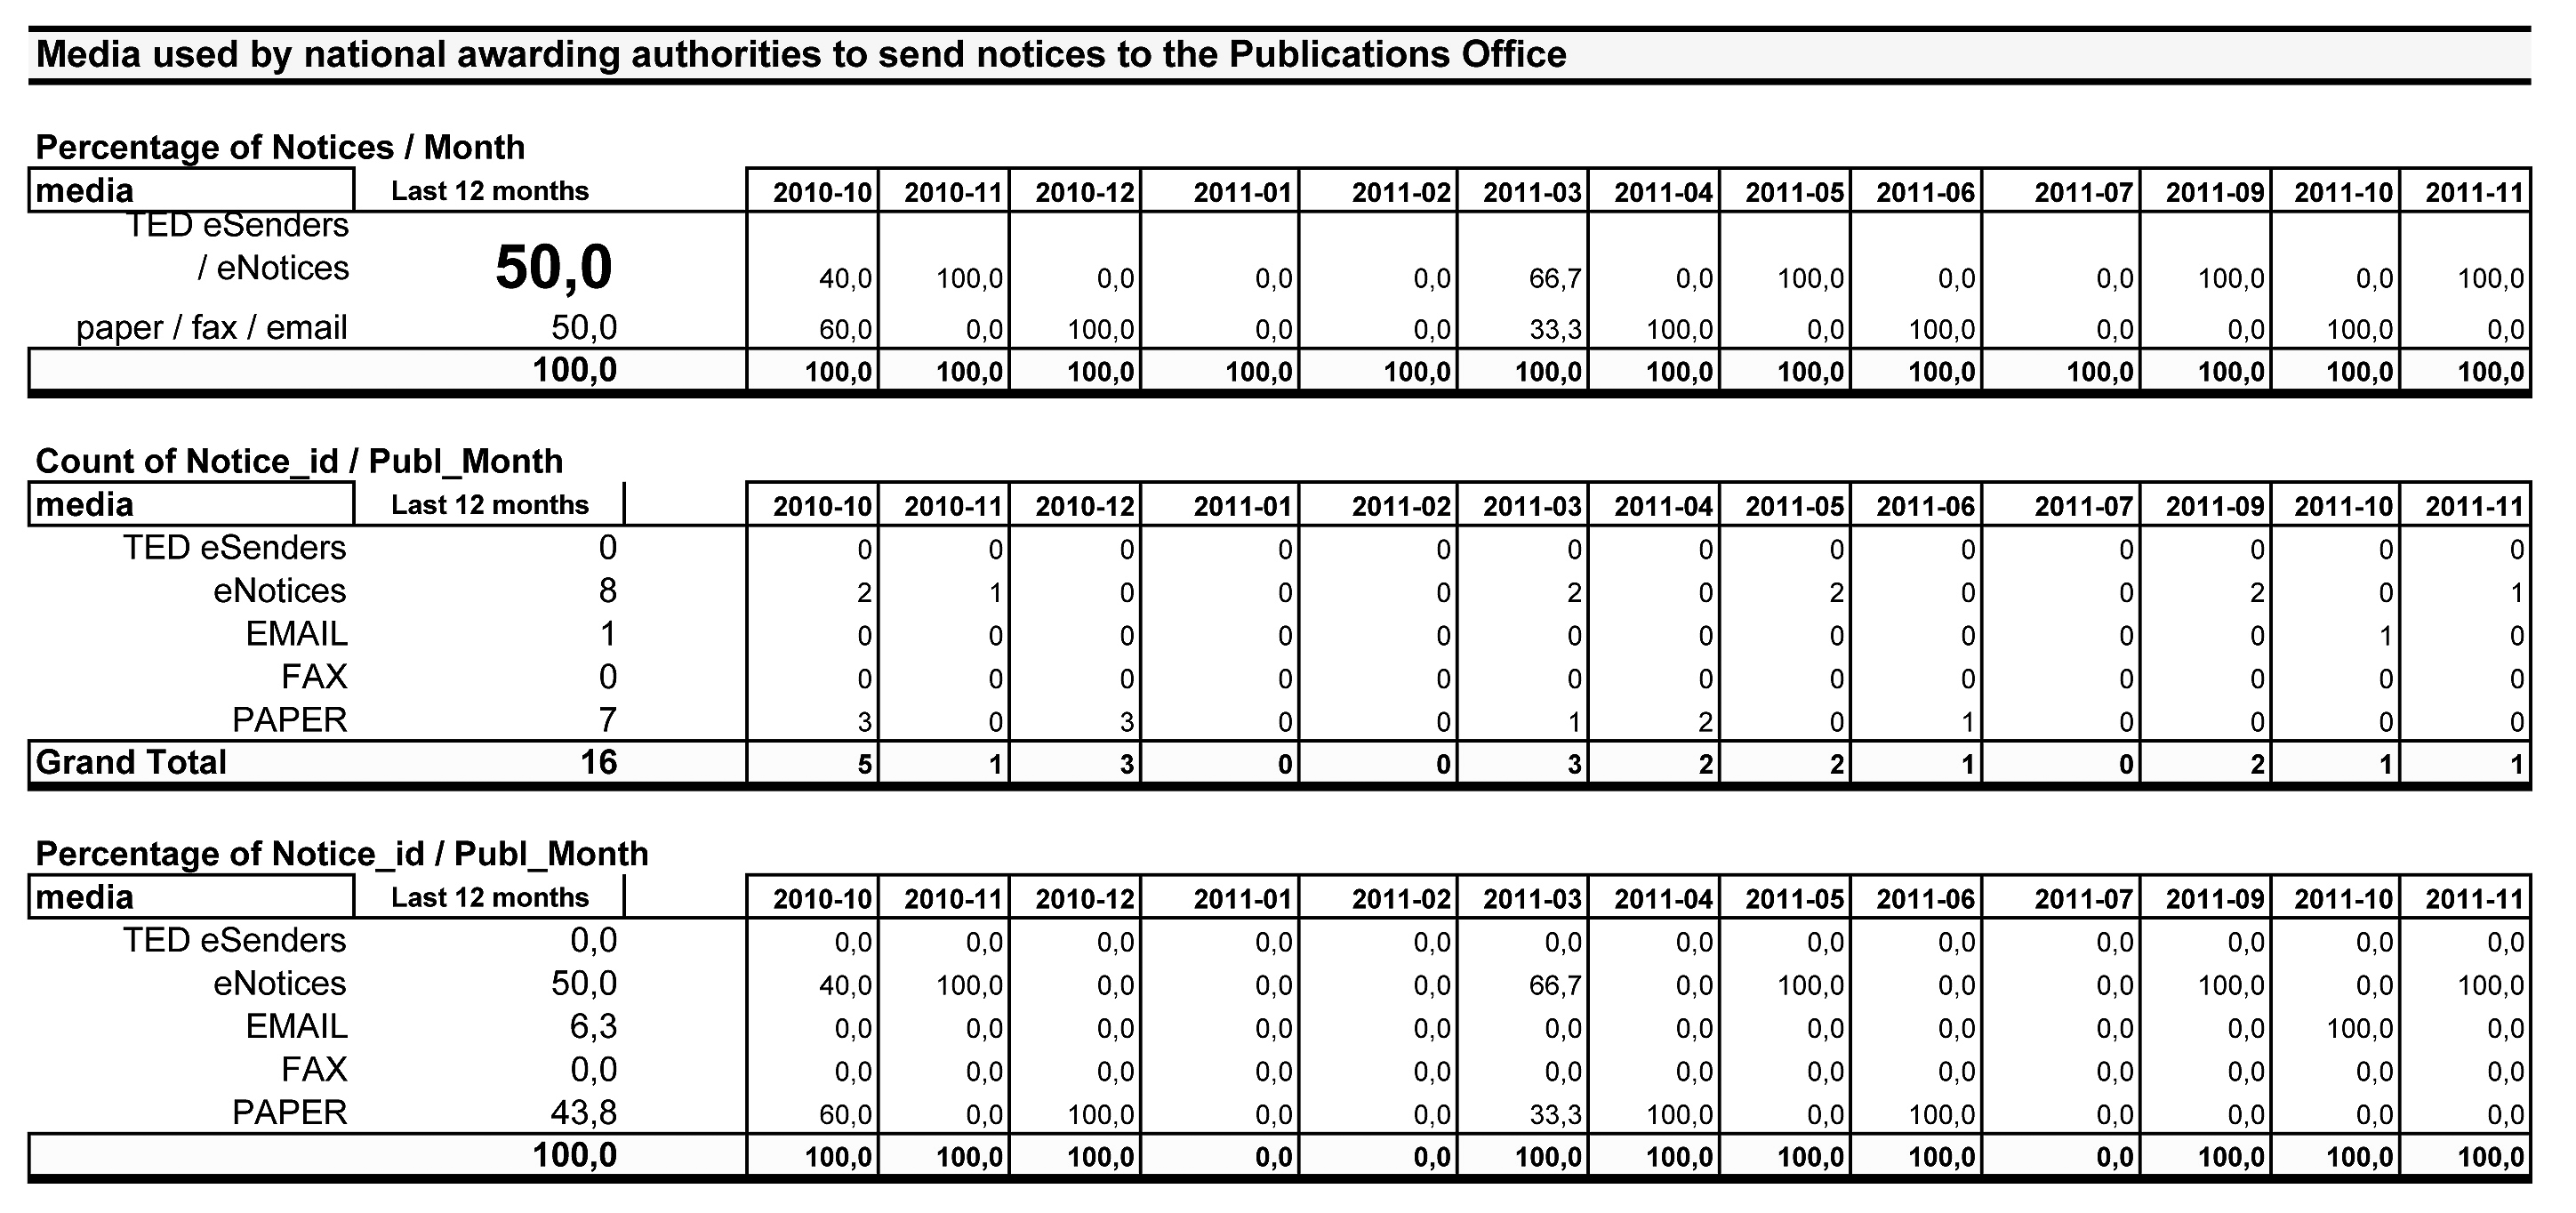
\includegraphics[width=16cm]{images/phd/eproc/circa-8}
\caption{Porcentaje y Tipo de Publicación de Anuncios de Licitación en TED de Turquía.}
\label{fig:circa-8}
\end{figure}


\item [\textit{eAccess}.] Esta fase cubre la habilidad de obtener copias de cualquier documento del 
proceso de contratación electrónica, incluyendo los anuncios de licitación. Los medios habituales
para posibilitar el acceso son la publicación a través de distintos sitios web o mediante correo
electrónico. Se trata igualmente de un proceso unilateral, cuya relevancia radica
en que las buenas prácticas y la estandarización deben estar presentes como puntos clave
para facilitar el acceso a la información de los anuncios de licitación.


\item [\textit{eSubmission}.] Esta fase trata el envío de las ofertas realizadas por un agente
económico al órgano de contratación. Se trata de un proceso bilateral en el cual se establece
una comunicación continua entre estos dos agentes. Unos de los principales desafíos radica
en el uso de sistemas de autenticación y autorización, que permitan la interoperabilidad
pan-europea entre los distintos sistemas de autenticación de los Estados miembros.

\item [\textit{eEvaluation/eAwarding}.] Estas dos fases desarrollan el proceso de toma de decisión
sobre qué oferta de las presentadas se ajusta mejor al pliego de condiciones técnicas. El desafío
clave en estas fases radica en el uso de técnicas totalmente automatizadas.

\item [\textit{eOrdering}.] Esta fase conlleva la tarea de automatizar el proceso de publicar la información
en línea, especialmente mediante el uso de catálogos (eCatalogues) que serán utilizados
posteriormente por las herramientas que dan soporte a las distintas fases.

\item [\textit{eInvoicing}.] Esta fase se encarga de la gestión de las facturas a través de medios
electrónicos. Su principal desafío radica en el uso de medios electrónicos para el tradicional 
proceso de facturación requiriendo la comunicación e interoperabilidad entre los agentes
participantes.

\item [\textit{ePayment}.] Esta fase está relacionada con la gestión de los pagos y las transferencias
de dinero entre los agentes participantes. Se trata por tanto de transacciones B2B, en las cuales
la seguridad es un factor clave. Por todo ello, se ha definido el \textit{Payment Services Directive}
como resultado del \textit{Single Euro Payments Area}, con el objetivo de eliminar posibles barreras
en los sistemas electrónicos de pago.
\end{description}

Atendiendo a estas definiciones y según la exposición realizada en este documento y trabajo de investigación
los resultados están orientados a mejorar tres fases de las identificadas por la Comisión: 
\textit{eNotification}, \textit{eAccess} y \textit{eOrdering}. No obstante, tratándose de la aplicación
de tecnología semántica con las características intrínsecas que conlleva, también se podrían aplicar
a otras fases con el objetivo de impulsar la interoperabilidad entre los agentes implicados en el proceso
de contratación electrónica.

\section{Marco legal en Contratación Publica}
El proceso de contratación pública electrónica se ha definido como clave en la Unión Europea, por ello
se han redactado diferentes reglamentos que deben ser transpuestos a la legislación de cada país para unificar
los criterios y establecer un marco común en todo el proceso. De esta manera, se establece una
base legislativa que da soporte, para que la contratación pública electrónica en la Unión Europea sea transfronteriza. Es importante
destacar que la legislación sobre contratos públicos se ve sometida a continuos cambios que permitan adaptar los procesos a las
necesidades de la propia Administración Pública y de los licitadores, de esta manera las distintas actividades de publicación,
adjudicación, caracterización de los tipos de contrato etc.,  se actualizan con el objetivo de adaptarse a la casuística que
va surgiendo y cambiando a lo largo del tiempo. A continuación, se dispone de una descripción sintética de 
la lista de los Reglamentos, Leyes, Reales Decretos, etc., más destacados que se han formalizado, 
ordenados por ámbito y fecha (de más a menos reciente):

\begin{itemize}
\item Reglamento (CE) Nº 1177/2009~\cite{r1177} de la Comisión, de 30 de noviembre de 2009 por el que se modifican las Directivas 2004/17/CE, 2004/18/CE y 2009/81/CE del Parlamento Europeo y del Consejo en lo que concierne a sus umbrales de aplicación en materia de procedimientos de adjudicación de contratos.

\item Reglamento (CE) Nº 1150/2009~\cite{r1150} de la Comisión, de 10 de noviembre de 2009 por el que se modifica el Reglamento (CE) no 1564/2005 en lo que respecta a los formularios normalizados para la publicación de anuncios en el marco de los procedimientos de adjudicación
de contratos públicos con arreglo a las Directivas 89/665/CEE y 92/13/CEE.

\item Reglamento (CE) No 213/2008~\cite{r213} de la Comisión, de 28 de noviembre de 2007 que modifica el Reglamento (CE) no 2195/2002 del Parlamento Europeo y del Consejo, por el que se aprueba el Vocabulario común de contratos públicos (CPV), y las Directivas 2004/17/CE y 2004/18/CE del Parlamento Europeo y del Consejo sobre los procedimientos de los contratos públicos, en lo referente a la revisión del CPV.

\item Directiva 2004/18/CE del Parlamento Europeo y del Consejo de 31 de marzo de 2004.

\item Real Decreto Legislativo 3/2011~\cite{rd3}, de 14 de noviembre, por el que se aprueba el texto refundido de la Ley de Contratos del Sector Público.
\item Ley 24/2011~\cite{l24}, de 1 de agosto, de contratos del sector público en los ámbitos de la defensa y de la seguridad.
\item Dictamen 31/11 de la Junta Consultiva de Contratación Administrativa sobre la obligatoriedad de integrar el perfil de contratante de los organismos y entidades del sector público estatal en la Plataforma de Contratación del Estado así como de las informaciones a publicar en la misma. 
\item Real Decreto 300/2011~\cite{r300}, de 4 de marzo por el que se modifica el Real Decreto 817/2009, de 8 de mayo, por el que se desarrolla parcialmente la Ley 30/2007, de 30 de octubre, de contratos del sector público y se habilita al titular del Ministerio de Economía y Hacienda para modificar sus anexos.
\item Ley 2/2011~\cite{l2}, de 4 de marzo, de Economía Sostenible.
\item Anteproyecto de Ley de Contratos del Sector Público en el ámbito de la Defensa y la Seguridad.
\item Ley 30/2007~\cite{l30} incorporando las modificaciones de la Ley 34/2010~\cite{l34}, y otras normas posteriores a su publicación.
\item Acuerdo de la Junta Consultiva de Contratación Administrativa en relación con los supuestos de derecho transitorio que pueden derivar de la entrada en vigor de la Ley 34/2010, de 5 de agosto .
\item Ley 34/2010~\cite{l34}, de 5 de agosto, de modificación de las Leyes 30/2007, de 30 de octubre, de Contratos del Sector Público, 31/2007, de 30 de octubre, sobre procedimientos de contratación en los sectores del agua, la energía, los transportes y los servicios postales, y 29/1998, de 13 de julio, reguladora de la Jurisdicción Contencioso-Administrativa para adaptación a la normativa comunitaria de las dos primeras.
\item Orden EHA/1490/2010~\cite{o1490}, de 28 de mayo.
\item Resolución~\cite{r3} de 3 de marzo de 2010, de la Dirección General del Patrimonio del Estado, por la que se 
publica la Recomendación de la Junta Consultiva de Contratación Administrativa sobre el envío de anuncios a la Comisión Europea. 
\item Orden EHA/3497/2009~\cite{oEHA}, de 23 de diciembre por la que se hacen públicos los
límites de los distintos tipos de contratos a efectos de la contratación administrativa a partir del 1 de enero de 2010.
\item Real Decreto 817/2009~\cite{rd817}, de 8 de mayo, por el que se desarrolla parcialmente la Ley 30/2007, de 30 de octubre, de Contratos del Sector Público. 
\item Instrumentos para la aplicación de la Ley 30/2007 de 30 de Octubre de Contratos del Sector Público.
\item Orden EHA/1220/2008~\cite{oEHA1220} de 30 de abril, por la que se aprueban las instrucciones 
para operar en la Plataforma de Contratación del Estado.
\item \ldots
\end{itemize}

En conclusión, se puede observar como las directivas europeas se transponen a los Estados Miembros,
en este caso España, con el objetivo de unificar en la medida de lo posible la gestión de la contratación pública
mediante medios electrónicos y así poder facilitar el acceso a la misma a las distintas empresas y personas de 
todos los \gls{Estados} Miembros en un mercado abierto común.

\section{Necesidades de e-Procurement}
Desde la Comisión Europea existe el compromiso firme de afianzar y desarrollar la contratación
pública electrónica~\cite{plan2004,e-Proc-green-paper,ePractice} con el objetivo de facilitar el acceso a los procesos administrativos a todas
las empresas interesadas en el mercado común. Con ello se pretende conseguir una serie
de ventajas que enlazan con las iniciativas de \textit{Open Government} (\gls{OG}), ver Sección~\ref{opendata-sect}:
\begin{itemize}
 \item Reducción de costes tanto temporales como materiales. Habitualmente un proceso
de contratación pública implica un gran despliegue de recursos humanos que deben dar 
soporte a las distintas actividades implicadas en el proceso administrativo y en las
comunicaciones con los participantes. Esta situación se puede agilizar y optimizar
para hacer un uso eficiente de los recursos propios de la administración y facilitar
la interacción con las entidades implicadas.
\item Incremento de la transparencia y accesibilidad. La automatización de los procesos
de contratación púbica centralizando los flujos de comunicación para concurrir a un concurso
de licitación mejora la transparencia de la Administración Pública, suministrando información
en un punto común y favoreciendo la accesibilidad a la misma, estableciendo el lugar 
en el cual encontrar la información. En general los costes de búsqueda de oportunidades
se agilizan y se hace mucho más abierto favoreciendo la divulgación a través
de la red global de Internet. Esto trae consigo un incremento de la competencia
ya que un mayor número de empresas pueden ser conscientes de las oportunidades de concurrir
a los procesos, impulsando la apertura del mercado y obteniendo ofertas más competitivas.
\item Mejora de la eficacia de la gestión administrativa. Dependiendo del tipo de contrato,
por ejemplo las centrales de contratación, los procedimientos pueden ser centralizados y de esta manera
ser racionalizados con una eficiente gestión de recursos.
\item Incremento de la integración entre mercados de la Unión Europea. El proceso
tradicional de contratación está basado en el uso de papel como modelo de intercambio
de información, con los consiguientes problemas asociados: multiling\"{u}ismo, localización, etc.,  
que impiden que las empresas puedan concursar más allá de su lugar de ubicación. El uso de la contratación
publica electrónica supera estas barreras tradicionales proveyendo un canal de comunicación
común, en el cual cualquier entidad dispone de las mismas oportunidades independientemente
de su país de procedencia. Con ello se consigue una participación transfronteriza
de las distintas empresas.
\end{itemize}

En general, estas necesidades y ventajas asociadas al uso de las tecnologías de la información
aplicadas al proceso de contratación pública deben contribuir a lograr una mayor eficacia
en el uso de los recursos de la Administración Pública y de las entidades participantes
en las distintas actividades. El contexto económico actual invita a reducir costes
corrientes, entre los que se encuentra el exceso de burocracia presente tanto en el ámbito de los recursos humanos como materiales. 
Teniendo en cuenta el volumen de contratos públicos en el ámbito europeo queda justificado que el impulso de la administración electrónica en este campo debe ser
prioritario. Por otro lado, la implantación de estos nuevos procesos, el coste del cambio, exige
fuertes inversiones tanto técnicas como de formación y difusión para concienciar a los distintos
agentes participantes del proceso de las necesidades y ventajas de este nuevo enfoque. Según
informes~\cite{e-Proc-green-paper} de la Unión Europea, el coste a escala nacional y regional
de la implantación de portales electrónicos de contratación se situaría entre $0,5$ y $5$ millones
de euros, el coste de mantenimiento de los mismos se estima~\cite{ePractice} entre miles y varios millones
de euros, dependiendo de la escala del sistema y la sofisticación del mismo.

\section{e-Procurement en la Unión Europea}\label{e-proc-eu}
El despliegue de un sistema de contratación pública a nivel europeo requiere
una fuerte inversión que debe recaer a nivel nacional y regional, ya que las necesidades
particulares y capacidades de cada entidad pública quedan de manifiesto en estos ámbitos.
Por otra parte, la legislación de la Unión \gls{Europea} en este campo permite a las entidades
adjudicadores seleccionar el método y canal de comunicación más apropiado de acuerdo
a su funcionamiento (electrónico o tradicional) si se ha sobrepasado un cierto umbral
de contratación. Es por ello que a nivel europeo la estrategia se sitúa en proveer
el marco legal necesario para liberar el mercado de la contratación pública mediante
una organización descentralizada y descoordinada con los siguientes objetivos:
\begin{itemize}
 \item Permitir a las entidades adjudicadores seleccionar el medio y canal para llevar
a cabo el proceso de contratación pública.
\item Asegurar que el proceso se desarrolla bajo las directrices de la Unión Europea
y de acuerdo a los tratados que fijan los umbrales de contratación y sus condiciones.
\item Fomentar el desarrollo de soluciones tecnológicas convergentes que permitan
la viabilidad electrónica del proceso dando lugar a una serie de buenas prácticas
que sean promocionables a otros servicios.
\item Facilitar la participación de las distintos agentes en un ámbito global a nivel
europeo eliminando en la medida de lo posible los costes de la contratación transfronteriza. Para ello
las soluciones técnicas deben asegurar la eliminación de barreras intrínsecas a la diversidad
europea, por ejemplo el idioma.
\end{itemize}

Enmarcando estos objetivos en una dimensión superior, la Unión Europea debe ejercer la función
de coordinación e impulso general del sector de la contratación pública, para armonizar un sector
altamente divergente pero de un gran calado para la economía de toda Europa. Hasta el momento las
medidas tomadas por la Comisión se centran en lo ya comentado sobre el aseguramiento del marco
legislativo. No obstante, han promovido ciertas acciones como: 1) la modificación
de ciertas Directivas de contratación pública que permitieran la introducción de técnicas
electrónicas y sistemas automáticos para la adquisición de bienes y servicios; 2) plan
de acción para que ``...cualquier empresa europea que disponga de un ordenador y una conexión a
 Internet pueda participar en una adquisición pública llevada a cabo con medios electrónicos.''
y 3) cofinanciación de investigación para el desarrollo de tecnología que permitiese
la contratación pública transfronteriza como las iniciativas \gls{PEPPOL}~\cite{peppol} y la herramienta e-CERTIS~\cite{e-certis}. Como ejemplo
de la actividad de la Unión Europea en este área y del Plan de Acción, el uso 
de \textit{Tenders Electronic Daily} (\gls{TED}) en el año 2009 superó el $90\%$ para las licitaciones
que superaban un cierto umbral, ver Tabla~\ref{umbralesTed}, generando $300$ \textit{billion} de euros en licitación. TED supone un gran avance para el campo de la contratación
pública electrónica proporcionando formularios estándar~\cite{formsTed} (19) para las distintas fases y herramientas que permiten
la gestión de la documentación e información como \textit{eNotices}~\cite{eNotices}. En resumen, las acciones identificadas en el Plan de Acción de 2004 
siguen vigentes hoy en día y el contexto de actuación sigue siendo clave para el impulso de la contratación
pública electrónica y la participación transfronteriza en la contratación 
en línea.

\begin{longtable}[c]{|p{7cm}|p{8cm}|} 
\hline
  \textbf{Tipo de Contrato} & \textbf{Umbral} \\\hline
\endhead
\textit{Public works} & $5,000,000$ \euro \\ \hline 
\textit{Service contracts}&$200,000$ \euro \\ \hline 
\textit{Supplies contracts}& $200,000$ \euro \\ \hline 
\textit{Supplies in the sectors of water, energy and transport}&$400,000$ \euro \\ \hline
\textit{Supplies in the telecommunications sector}&	$750,000$ \euro \\ \hline 
\textit{Contracts falling under the GATT agreements}&	$130,000$ \euro \\ \hline
 \hline
\caption{Tipos de Contratos y Umbrales para publicar en TED.}\label{umbralesTed}\\    
\end{longtable}


\section{Desafíos europeos en e-Procurement}
Las ventajas y necesidades revisadas anteriormente implican una serie de retos a distintos
niveles que suponen una barrera de entrada a la adopción integral de las soluciones basadas
en tecnologías de la información para los procesos de contratación pública. Por ello,
se fijan distintos puntos de acción que deben ser abordados para conseguir la implantación
exitosa de la administración electrónica en el campo de los contratos públicos.

\begin{itemize}
 \item Uno de los principales problemas en relación a la implantación de un nuevo proceso consiste en la 
concienciación al cambio tanto a las entidades adjudicatarias como a los posibles proveedores. La inercia
en la Administración Pública habitualmente conlleva una lenta adopción de los nuevos trámites, debido
a cuestiones de reorganización interna y desconocimiento de las nuevas ventajas. Por otra parte, 
la reacción de los proveedores cuando interactúan con la Administración, en una situación de transición ,
suele venir marcada por cierto escepticismo debido a la falta de confianza
en las nuevas tecnologías, la pérdida de la interacción personal, etc. Especialmente en este
tipo de operaciones de centralización, las \gls{PYME} suelen inquietarse por el temor a caer en un 
estado de obsolescencia en su relación con la Administración. Es por ello que la
capacidad de concienciación por parte de la Administración Pública al entorno afectado, se plantea
como un reto crítico.

\item Homogeneización de la normativa aplicada a la contratación pública electrónica. Como
se ha comentado en anteriores secciones la Unión \gls{Europea} a través de distintas Directivas
marca el paso que han de seguir los distintos \gls{Estados} Miembros para transponer la normativa
a sus entornos nacionales y regionales. Sin embargo, la aparición de numerosas plataformas
y casos particulares de contratación conllevan una complicación superior a los proveedores
candidatos a concursar. Por ejemplo en el caso de la fase de presentación de las ofertas, 
el aprendizaje necesario para el uso de estos nuevos portales opera como una importante
barrera de entrada a los procesos. En este punto, la Unión Europea actúa con el objetivo
de normalizar al máximo los procesos transfronterizos con la intención de unificar criterios
y obtener sistemas interoperables que no confundan a sus usuarios. Algunas de estas líneas
transversales se centran en la autenticación de usuarios, intercambio de documentación,
facturas, catálogos, etc., de forma estándar.

\item Enredo de requisitos técnicos que impiden la adopción ágil de los nuevos procesos. El típico
caso se ve reflejado en los sistemas de autenticación e identificación que van desde la simplicidad de un 
par, usuario y contraseña, hasta sistemas más complejos basados en firma o certificados
digitales. 

\item Adopción paulatina. Las capacidades y prioridades de cada Estado Miembro varían dependiendo
de distintos parámetros y aunque el objetivo final es la implantación completa e integrada en cada
uno de los países, cada uno de ellos avanza con su propio ritmo. No obstante, cabe resaltar
que el desafío reside en que paulatinamente todos los instrumentos necesarios para la contratación
transfronteriza se hagan realidad mediante este esfuerzo común.
\end{itemize}

La Unión Europea, como órgano integrador y vertebrador de los distintos Estados Miembros, tiene la obligación
de aunar y coordinar los esfuerzos nacionales y regionales para la adopción definitiva de la contratación
pública electrónica dando respuesta tanto a las necesidades como a los retos que esta iniciativa conlleve.

\section{Iniciativas y proyectos en e-Procurement}
Dentro del Plan de Acción realizado en 2004 para el impulso de la contratación pública electrónica, se habían
seleccionado diferentes líneas de actuación que se han materializado en actividades a lo largo de estos años algunas de las cuales ya se han 
dado por finalizadas mientras que otras siguen su curso. Atendiendo 
al mapa de actividades~\cite{e-Proc-map-paper} realizadas podemos destacar las siguientes:

\begin{enumerate}
 \item \textbf{e-Certis}. Herramienta de información en línea y gratuita que
se ha lanzado en las últimas fechas (2010) para aportar datos sobre los
diferentes tipos de certificados y declaraciones que se suelen exigir
en los procedimientos de contratación de los 27 \gls{Estados} miembros, los países
candidatos (Turquía y Croacia) y los países del \gls{EEE} (Islandia, Liechtenstein y Noruega). 
La principal función de esta herramienta es ayudar a los agentes económicos y a las
entidades adjudicadoras a comprender qué tipo de información se solicita, así como facilitar
la información aceptable. Esta acción sigue su curso, siendo el órgano responsable
\textit{The Internal Market and Services Directorate General} (\gls{DG-MARKT}), centrando su aplicación 
en la fase de \textit{eTendering} (\textit{eAttestation}).
\item \textbf{Fiscalis 2013}. Esta iniciativa trata de luchar contra el fraude
fiscal, mejorar las prácticas administrativas y asegurar el intercambio de información
entre las Agencias Tributarias nacionales y las entidades adjudicatarias, a través
de los sistemas transfronterizos de fiscalidad. Es una acción iniciada en el año 2008
y cuyo plazo de finalización está previsto para el año 2013. Es el órgano responsable \textbf{Taxation and Customs Union} (\gls{DG-TAXUD}) y 
su principal aplicación se centra en las fases de: \textit{eInvoicing} y \textit{ePayment}.
\item \textbf{\gls{ePRIOR}}. Se trata de la implementación de servicios interoperables
electrónicos a nivel europeo para la fase posterior a la adjudicación del contrato
público. A través del programa \textit{Interoperable Delivery of European eGovernment Services to public Administrations, Businesses and Citizens}(IDABC) y \textit{eInvoicing} y \textit{eOrdering}, iniciados
en verano del año 2007 por el \gls{DG-MARKT} y \textit{Directorate-General for Informatics} (\gls{DIGIT}) 
de la Comisión Europea, buscan contribuir a los objetivos de la iniciativa \textbf{i2010} mediante el establecimiento
de un marco de políticas comunes para la sociedad de la información y medios digitales. Se ha
realizado un prototipo en el cual se han incluido la metodología RUP@EC, se ha realizado
un estudio sobre el uso de \textit{eCatalogues} y se ha desarrollado un conector
a la infraestructura del proyecto PEPPOL. Como resultado principal se ha obtenido
el despliegue de la plataforma \gls{ePRIOR} (\textit{electronic PRocurement Invoicing and
ORdering}) en octubre del año 2009. Los órganos responsables son el \gls{DG-MARKT} y \gls{DIGIT} cubriendo
las fases o temas de \textit{eInvoicing}, \textit{eOrdering} y \textit{eCatalogues}.
\item \textbf{Open e-PRIOR}. Es la versión de la iniciativa anteriormente mencionada, 
en la cual los formatos de fuente son abiertos, permitiendo el intercambio
de información y documentos a través de la infraestructura \gls{PEPPOL}. Tanto los
órganos responsables como las fases cubiertas son las mismas que en el caso precedente.
\item \textbf{PEPPOL - Pan-European Public Procurement Online}. Es el gran proyecto
de contratación pública electrónica transfronteriza gestionado por organismos del 
sector público de diferentes países y cofinanciado por la Unión \gls{Europea}. Su principal
objetivo es disponer de una infraestructura para facilitar el despliegue de servicios
tecnológicos en un entorno homogéneo y de escala global para el desarrollo y la gestión
de las operaciones implicadas en los procesos de contratación pública paneuropea. El núcleo
de este proyecto lo constituye una red de transporte que permite a los socios comerciales
conectar sus recursos tecnológicos para el intercambio de documentos de forma segura
y fiable. También se considera su aplicación para los pedidos, la facturación 
electrónica, firma y validación, expedientes virtuales para la empresa, creación
de catálogos electrónicos, etc. El órgano responsable es \textit{The Information Society and Media Directorate General} (\gls{DG-INFSO}) (CIP ICT/PSP programme)
y las fases cubiertas por este proyecto corresponden a \textit{eOrdering}, \textit{eInvoicing}, 
\textit{eCatalogue} y \textit{eSignature}. Este proyecto, debido a su gran envergadura se encuentra
dividido en diferentes paquetes de trabajo (8), cubriendo diferentes fases y colaborando
con otras iniciativas tales como: \textit{WP1- eSignature, WP2- Virtual Company Dossier, WP3 – eCatalogue,
WP4 –eOrdering, WP5- eInvoicing, WP6-Project Management, WP7- Consensus and awareness building
y WP8- Solutions architecture, design and validation}. De esta forma y a través
de los subproyectos se cubren nuevas etapas de la contratación como  
\textit{eNoticing, eTendering, eAwarding y eOrdering}.
\item \textbf{\gls{STORK} - Secure idenTity acrOss euRope linKed}. El objetivo de esta iniciativa
es establecer ``...a European eID Interoperability Platform'', que permita a los ciudadanos y 
a las empresas establecer relaciones virtuales transfronterizas a través del uso 
de los documentos de identificación nacionales. El órgano responsable de esta acción
es el \gls{DG-INFSO} y cubre las fases de \textit{eSignature} y \textit{eID}.

\item Iniciativas en el campo de la estandarización que se han realizado
a lo largo de los años entre las que podemos destacar:
\begin{itemize}
 \item \textit{CEN BII - Workshop on 'Business Interoperability Interfaces on public procurement in Europe' Phase 2 (WS/BII 2)}.
\item \textit{CEN eCAT - Multilingual eCataloguing and eClassification in eBusiness}.
\item \textit{CEN WS/eBES - Workshop on 'e-business Board for European Standardization'}.
\item \textit{CEN - Workshop on eInvoicing Phase 3 (CEN WS/INV3)}.
\item \textit{OASIS TC/UBL - The Universal Business Language}.
 \item \textit{UN/CEFACT - United Nations Centre for Trade Facilitation and Electronic Business}. En los grupos de trabajo
específicos de \textit{International Trade and Business Group (TBG)} y en concreto, \textit{TBG1 - Supply Chain},
\textit{TBG6 – Architecture, Engineering and Construction} y \textit{TBG19 - \gls{eGovernment}}.
\end{itemize}

\item Participación en otros grupos de trabajo, comunidades y redes de trabajo como \textit{eProcurement Forum}.
\end{enumerate}

Finalmente y dentro de esta gran actividad de han completado proyectos de diversa índole como:
\textit{Evaluation of eProcurement uptake} (encuesta en línea) y \textit{CROBIES - Cross-Border Interoperability of eSignatures},
participado en foros de discusión: \textit{CEN eBIF - European e-Business Interoperability Forum} y
\textit{CEN BII - Workshop on ``Business Interoperability Interfaces on public procurement in Europe'' Phase 1}, redactado
documentos estratégicos \textit{``Evaluation of the 2004 Action Plan for Electronic Public Procurement''} (2010),
\textit{``Green Paper on expanding the use of eProcurement in the EU''} (2010), 
\textit{``Summary of the responses to the Green Paper on expanding the use of eProcurement in the EU''} (2011), 
\textit{``Reaping the benefits of electronic invoicing for Europe''}, \textit{``e-Catalogues Gap Analysis between pre-awarding business requirements 
and the post-awarding implementation in e-PRIOR, Version 1.0''}, etc., mediante los cuales se ha intentado
concienciar a la comunidad sobre las ventajas del impulso de la contratación pública electrónica, utilizando
estándares y las nuevas tecnologías de la información. Como ya hemos comentado, siempre enclavadas en un marco
legislativo referente \textit{``New Directive on eInvoicing''} (2010) o 
\textit{``Provisions relating to eProcurement introduced by the public procurement Directives 2004/17/EC13 and 2004/18/EC14''} (2004) y también
otros como el \textit{``New Common Procurement Vocabulary''} (2008).

En conclusión, se puede observar como la actividad de la Unión Europea en este campo y de sus distintos organismos, 
apuesta ciegamente por el impulso de la contratación pública electrónica como medio para la mejora de la economía
y de la competitividad en un ámbito paneuropeo, en el cual las tecnologías de la información y los estándares 
juegan un papel clave. La financiación de todas estas actividades requiere un esfuerzo común de las administraciones
nacionales y regionales pero el retorno es evidente tanto para las empresas, ciudadanos, como para la propia
Administración ya que se consigue una mejora en toda la cadena valor en la que un contrato público actúa.

\section{Modelo de Información para los Anuncios de Licitación}
Una de las principales líneas de actuación para el impulso de la contratación
pública electrónica es disponer de sistemas interoperables con la capacidad de
comunicarse entre sí e intercambiar documentación, información y datos. Las propuestas
e iniciativas relacionadas en la sección anterior se centran en estos puntos. De
esta manera, en las etapas de contratación pública, ver Figura~\ref{fig:ted-1}, se produce un flujo constante de información entre las entidades
licitadoras y las partes licitantes (personas físicas o jurídicas). La flexibilidad y la capacidad
de procesamiento automática de toda esta información es clave para el impulso de la contratación
pública electrónica. Teniendo en cuenta que las barreras tecnológicas se pueden salvar utilizando
productos y herramientas en un estado de madurez alto, el principal problema se constituye en la interoperabilidad.

\subsection{Necesidad de Interoperabilidad}
La interoperabilidad es una característica de los sistemas que se define como la capacidad para compartir y hacer uso de la
información~\cite{interoperability}. No debería considerarse desde un único punto de vista, 
sino que también tiene connotaciones en relación con la experiencia de usuario en el
sentido de satisfacer las expectativas de los usuarios en cuanto al intercambio
y utilización de la información entre diferentes dispositivos y proveedores.
Además, un entorno interoperable mejora las relaciones económicas entre las
empresas ya que facilita su comunicación en entornos heterogéneos e impulsa las
relaciones \gls{B2B}.

\textit{The ability of two or more systems or components to exchange information
and to use the information that has been exchanged.}

En el actual entorno de ejecución como es la Web y con el despunte
de las arquitecturas orientadas a servicios (\gls{SOA}), la interoperabilidad es una de las claves para mejorar la comunicación
entre los componentes. La agilidad proveniente de un entorno interoperable conlleva una mejora importante en los distintos procesos que engloba SOA:
despliegue de nuevos servicios, evolución de la plataforma, etc. Las aplicaciones necesitan un entorno interoperable para mejorar su capacidad de
evolución y no caer en la obsolescencia. Como ejemplo se puede pensar en una nueva aplicación que realiza un servicio totalmente innovador, 
suponemos igualmente que otra aplicación, estaría interesada en utilizar este servicio por la ventaja que 
podría obtener con respecto a sus competidores. Si no se dispone de un entorno interoperable para comunicar estas dos aplicaciones, la ventaja competitiva de
las mismas decae y se necesitan aplicar recursos en tareas que podrían ser más o menos automatizadas en un entorno interoperable. Algunos de
los puntos de la necesidad de la interoperabilidad en SOA son los siguientes:

\begin{itemize}
 \item Mejorar la comunicación entre aplicaciones.
 \item Homogeneizar un entorno heterogéneo en cuanto a formato de datos y protocolos de comunicaciones.
\item Aplicar estándares acordados de forma comunitaria.
\item Agilizar los procesos de desarrollo y de mantenimiento.
\item Facilitar los entornos de pruebas.
\item Reutilizar lógica de negocio.
\end{itemize}

Desde un punto de vista técnico, podemos identificar dos tipos de interoperabilidad en el ámbito del software y las comunicaciones:
\begin{description}
\item [Sintáctica.] Sucede cuando los sistemas son capaces de intercambiar información 
en un formato de datos determinado y bajo unos ciertos protocolos de
comunicaciones. El caso más habitual es el uso de un vocabulario XML compartido
para expresar los datos. Es la base de la interoperabilidad entre aplicaciones en
los actuales entornos distribuidos.
\item [Semántica.] Más allá de la capacidad de intercambiar datos bajo ciertas
condiciones existe la posibilidad de la interpretación automática de los
mismos. Cuando las aplicaciones son capaces de compartir datos (sintaxis) e
interpretarlos automáticamente (semántica) conseguimos este tipo de
interoperabilidad. El valor añadido de la semántica a las aplicaciones se
aplica a su autonomía. En un entorno como SOA, existen ciertas operaciones
(descubrimiento o selección de servicios) que se pueden automatizar en un estado
consciente, aumentando el grado de flexibilidad de la arquitectura. Por otro
lado, la adición de semántica tiene que estar en buena relación con el
determinismo o la precisión de las operaciones que la usan, es decir, añadir
semántica en un entorno y trabajar con incertidumbre no tiene sentido para
ciertas operaciones. 
\end{description}

La importancia de la interoperabilidad queda por tanto probada en el
sentido de fluidificar la comunicación entre distintas aplicaciones, es decir,
que ``hablen'' el mismo lenguaje. Esta característica dentro de las
arquitecturas globales es esencial, ya que junto a la integración se mejora por un
lado la comunicación de aplicaciones y el formato de las mismas. En el
momento en el que aparecen heterogeneidades se pueden utilizar adaptadores de un
formato a otro, por lo que no representa en sí un gran problema si hemos fijado
las características anteriores.

\subsubsection{Cómo conseguir Interoperabilidad}
Para conseguir un entorno interoperable se pueden seguir una serie de acciones que mejoran la comunicación de las aplicaciones. Podemos
destacar las siguientes:

\begin{itemize}
\item Uso de estándares. Los estándares representan esfuerzos comunitarios en
cierto sector de negocio para mejorar la comunicación entre los distintos
sistemas. En este sentido, como paradigma se puede citar \textit{eXtensible Business
Reporting Language}  (\gls{XBRL}), el cual nace de la
propuesta lanzada en 1998 por Charles Hoffman, experto contable y auditor, para
simplificar la automatización del intercambio de información financiera mediante
el uso del lenguaje \gls{XML}. La idea subyacente en esta iniciativa no era otra que la
de estandarizar el formato con el que la información financiera se distribuye
entre los diferentes proveedores y consumidores.

\item Tecnología común de comunicaciones. Para transportar la información
utilizando cierto estándar establecido se debe utilizar un protocolo de
comunicaciones común. Por ejemplo, en los servicios web se utiliza
\gls{SOAP}~\cite{SOAP11} (peticiones \textit{\gls{POST}} sobre \gls{HTTP}) o \gls{REST}~\cite{rest}.

\item Implementaciones usando estándares. Las aplicaciones dispuestas al uso de
un determinado estándar, por ejemplo servicios web \gls{WSDL}~\cite{WSDL}+SOAP, deben realizar un
esfuerzo para saber trabajar con esos datos y adaptarlos a su lógica de negocio.
En resumen, las aplicaciones deben ser capaces de importar y exportar datos
utilizando los estándares propuestos.
\end{itemize}

\subsubsection{Semántica e Interoperabilidad}
La semántica representa un esfuerzo en cuanto a la consecución de la
interoperabilidad, tanto desde el punto de vista de la obtención de modelos de datos
comunes como de proporcionar los mecanismos adecuados para que la información
pueda ser procesada de forma automática por las aplicaciones. La aplicación de
semántica para mejorar la interoperabilidad se ve reflejada en diferentes
ámbitos: modelar el conocimiento de un dominio de forma estándar, utilizar este
modelo para describir los servicios del dominio o establecer un formato de
datos estándar. 

\begin{itemize}
\item Modelo de datos y formato estándar.
\item  El contenido es usable desde que está disponible.
\item  Es un formato procesable por las máquinas.
\item La información existente es fácilmente representable.
\item Flexibilidad en la representación de la información.
\end{itemize}

La aplicación de semántica en el campo de la contratación pública
electrónica será desarrollada dentro del contexto de este documento
en los siguientes capítulos y más específicamente en el Capítulo~\ref{capitulo:eproc-sm}.

\subsection{Propuestas y Modelos de Información actuales}\label{data-model-eproc}
Una vez revisado el concepto de interoperabilidad y su necesidad de aplicación
en el contexto de la contratación pública electrónica, teniendo en cuenta
la diversidad de plataformas para el proceso de contratación, modelos de información para definir las distintas
fases de \eproc y las iniciativas en desarrollo que se están promoviendo desde la Unión
Europea para ser transpuestas a nivel nacional y regional, es conveniente señalar que recomendaciones
se siguen actualmente.

A nivel europeo el modelo desarrollado en TED es preceptivo para los anuncios de licitación
que superen cierto umbral, ver Sección~\ref{e-proc-eu}, en el desarrollo de esta iniciativa
se ha conseguido interoperabilidad a nivel sintáctico, suministrando una serie de \gls{XML Schema}s que 
permiten establecer un modelo común para la información contenida en los anuncios de licitación. Actualmente,
estos \gls{XML Schema}s no están disponibles de forma pública, salvo que se disponga de una suscripción a la herramienta
eSenders, en su caso se pueden encontrar guías de implementación. 


\begin{figure}[!htb]
\centering
	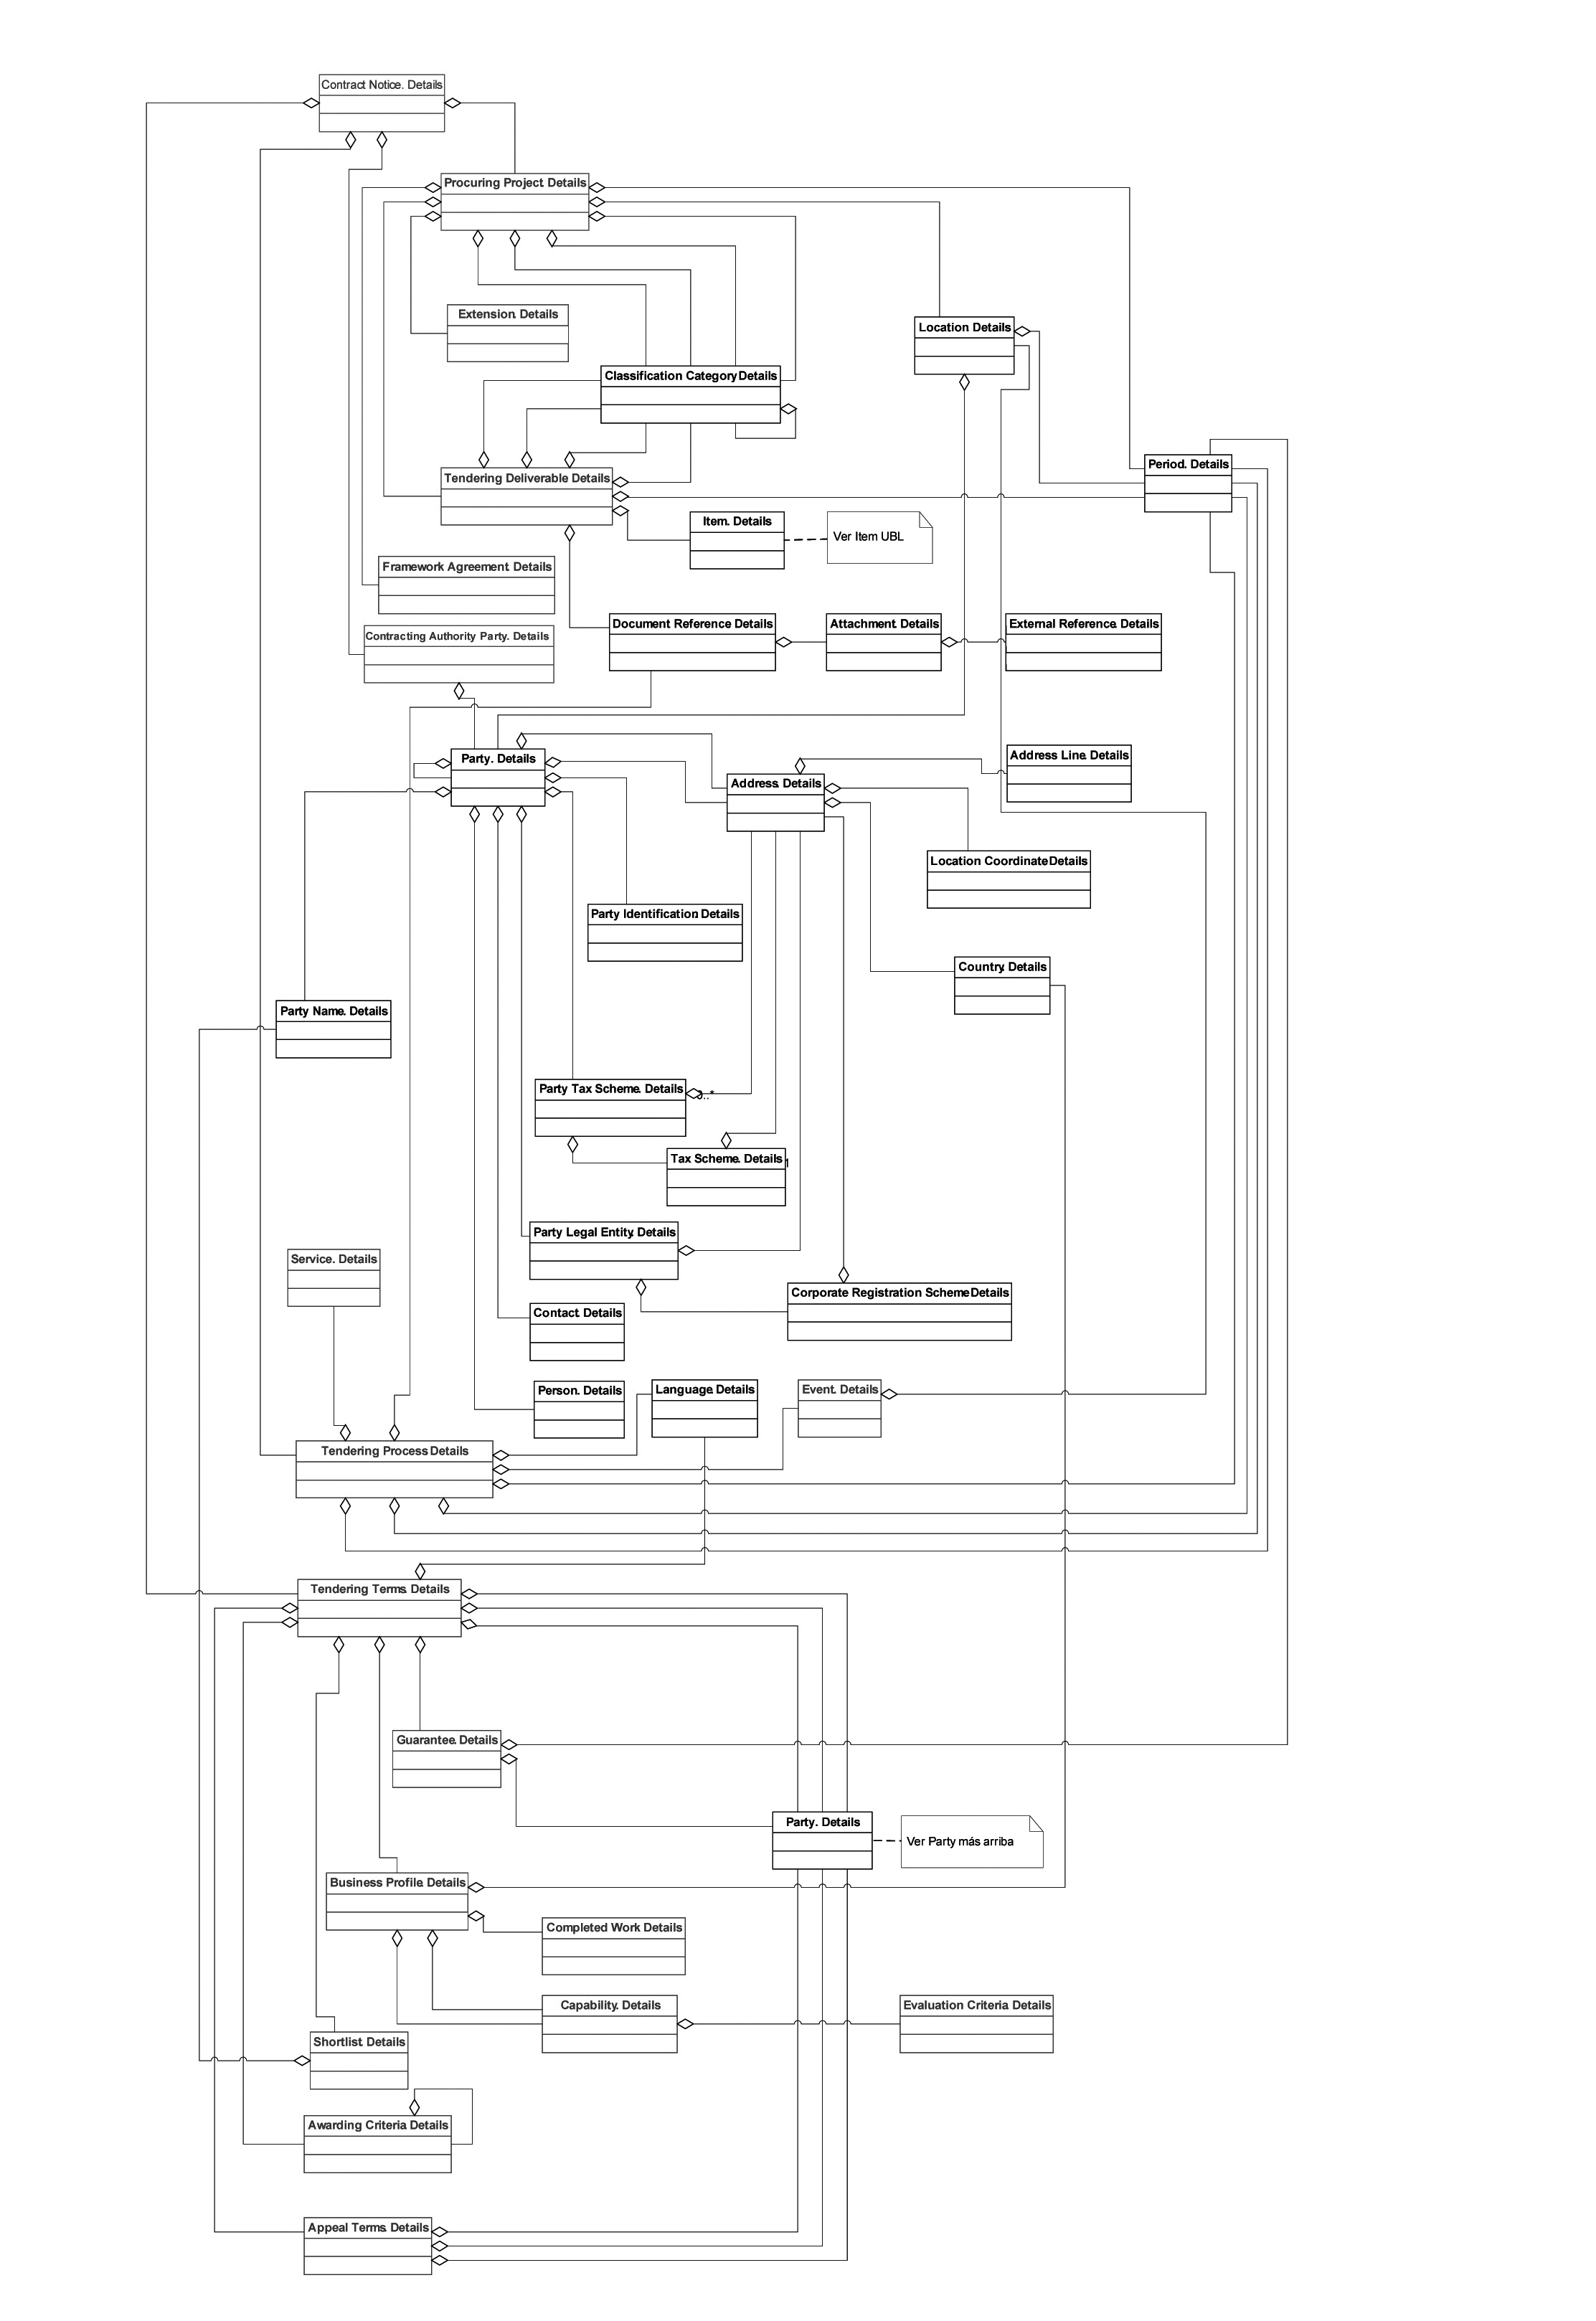
\includegraphics[width=14cm]{images/phd/eproc/codice-1}
\caption{Modelo de Información de Anuncio de Licitación en CODICE v1.}
\label{fig:codice-1}
\end{figure}


A nivel nacional, se puede utilizar como paradigma la Plataforma de Contratación del Estado 
que de nuevo han diseñado una serie de XML Schemas que permiten establecer un modelo formal
para todas las fases de e-Procurement. En concreto, para las fases que son objeto
de estudio en este documento: \textit{eNotification} y \textit{eAccess} podemos
encontrar el siguiente diagrama de componentes \gls{CODICE} v1, ver Figura~\ref{fig:codice-1}. De igual
forma, existen modelos similares, hasta 15 (\textit{Appeal Notification, Awarded Notification, Contract Award Notice, Contract Documents, Contract Documents Request,
 Contract Notice, Declaration, Guarantee Document, Invitation to Tender, Prior Information Notice, Qualification Result Notification, 
Rectification Request, Tender, Tender Reception Notification} y \textit{Unawarded Notification}), para cada una de las fases implicadas en 
el proceso de contratación pública electrónica, ver Figura~\ref{fig:codice-3}. En todos ellos se utilizan 
vocabularios \gls{XML} estándar como \textit{Universal Business Language} (\gls{UBL}), códigos \gls{ISO} para identificar monedas y países, etc., 
con el objetivo presente de la interoperabilidad como máxima para impulsar el uso de estas
plataformas.  A nivel regional, la casuística vuelve a ser diversa dependiendo de distintos 
modelos de información basados en diferentes modelos formales.


%
\begin{figure}[!htb]
\centering
	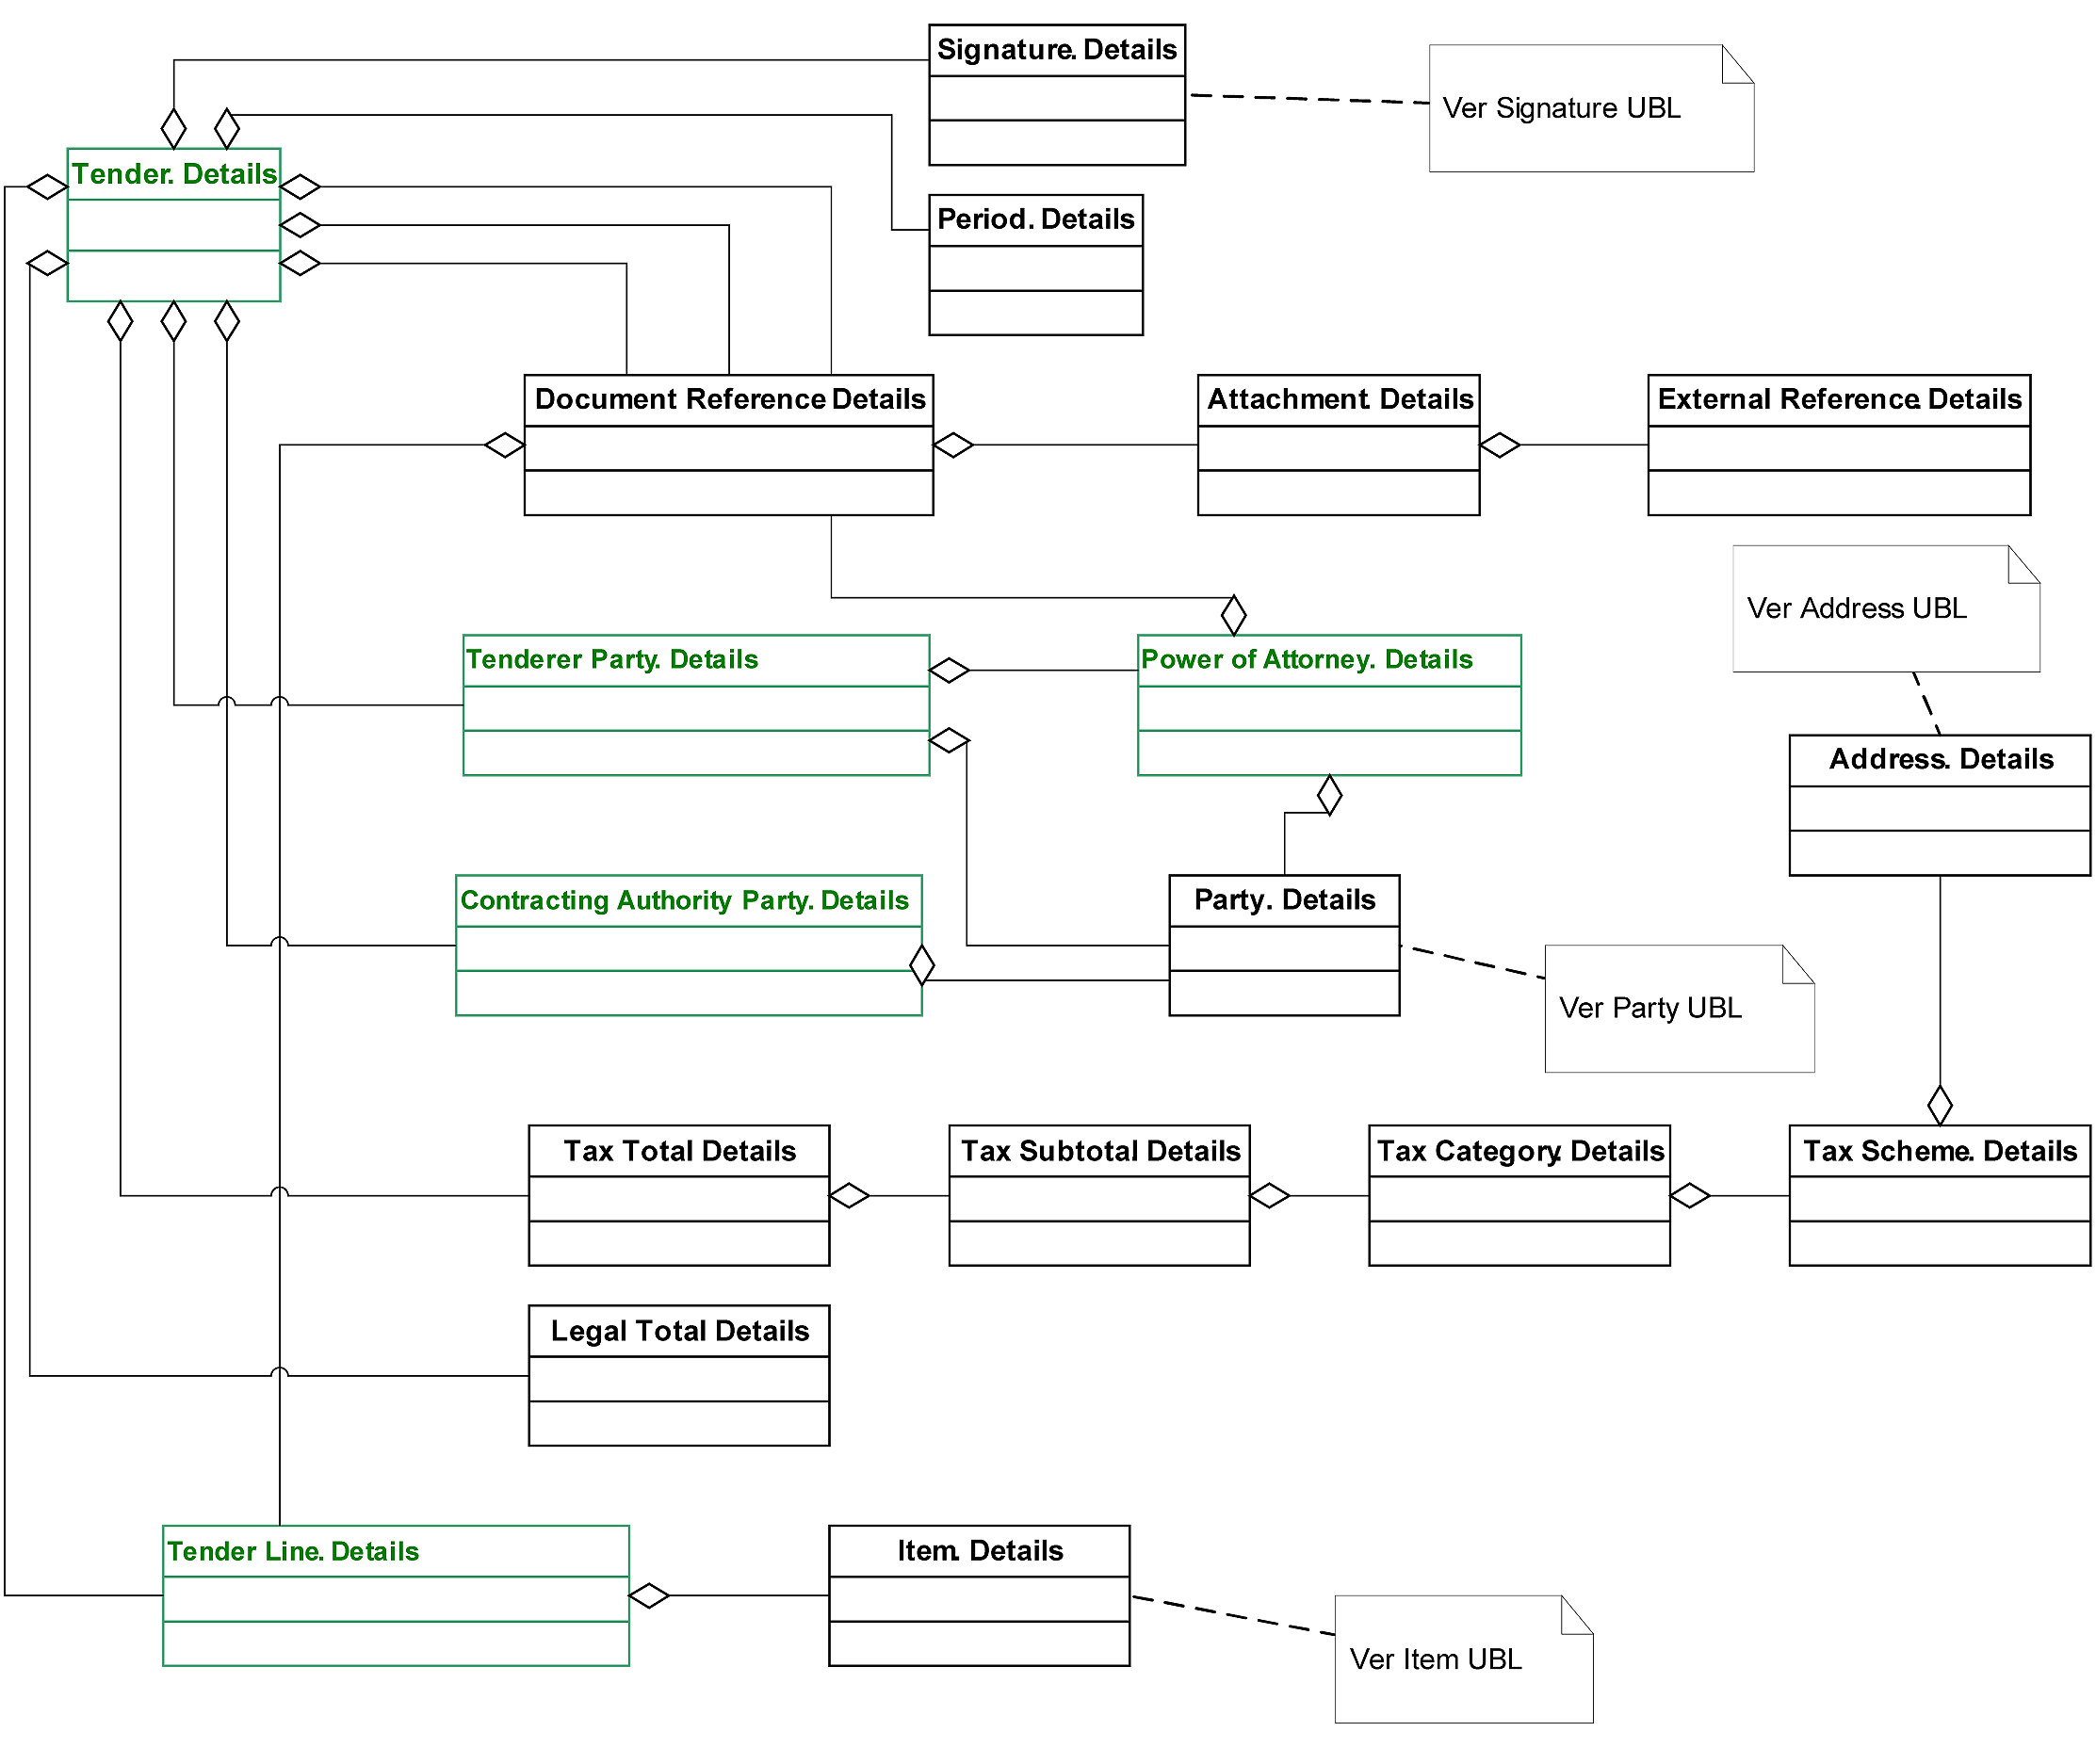
\includegraphics[width=16cm]{images/phd/eproc/codice-3-tender}
\caption{Modelo del Proceso de Contratación Pública Electrónica en CODICE v1.}
\label{fig:codice-3}
\end{figure}

El principal problema de todos estos modelos reside en la sobre-especificación
que se realiza de la información. La necesidad de que las distintas herramientas accedan
a diferentes datos obliga a modelar con un grado de especificidad muy alto cada tipo de dato, proporcionando
además una gran cantidad de metainformación. Todos estos esquemas siguen este modelo y realmente
son extremadamente difíciles de generar y tratar, especialmente para terceras partes interesadas
en acceder a esta información. Si bien supone un gran avance para la contratación pública electrónica, 
también en muchas ocasiones supone una considerable barrera de entrada ya que llega a comprender toda la información
necesaria, etc., requiere un enorme esfuerzo integrador que conlleva que posibles agentes involucrados
en el consumo de esta información no estén dispuestos a realizar. 

Esta situación ha sido identificada dentro del proyecto \textit{\gls{10ders} Information Services} y por ello
se ha desarrollado un nuevo vocabulario \gls{XML} con el objetivo de aunar la información de los anuncios de licitación,
contratos, etc., intentando unificar la versiones previas de \gls{TED}, \gls{CODICE} v1 y v2 y modelos
regionales. Este trabajo se ha plasmado en la creación de \textit{\gls{opXML}} que, nuevamente, incluye
una serie de modelos en \gls{XML Schema} para expresar dicha información. El objetivo principal
es servir como elemento vertebrador para expresar la información de forma común. Evidentemente,
es similar a las especificaciones previas pero busca una definición más sencilla que sea más manejable
por terceros y que tenga transformación directa con las distintas plataformas de contratación. La principal ventaja
es que surge por parte de una empresa experta en el dominio. Por otra parte, las desventajas
de este enfoque residen en que reiteradamente se define un vocabulario XML cuando ya existen varios en \gls{TED}, CODICE, etc., 
con este objetivo y no existe ningún consenso con otras entidades como puede ser la propia Administración o proveedores
de servicios.  A continuación y en contraste con los modelos anteriores de información se puede observar el 
enfoque seguido en \textit{opXML}, ver Figuras~\ref{fig:10ders-2},~\ref{fig:10ders-1} y~\ref{fig:10ders-6}. 


\begin{figure}[!htb]
\centering
	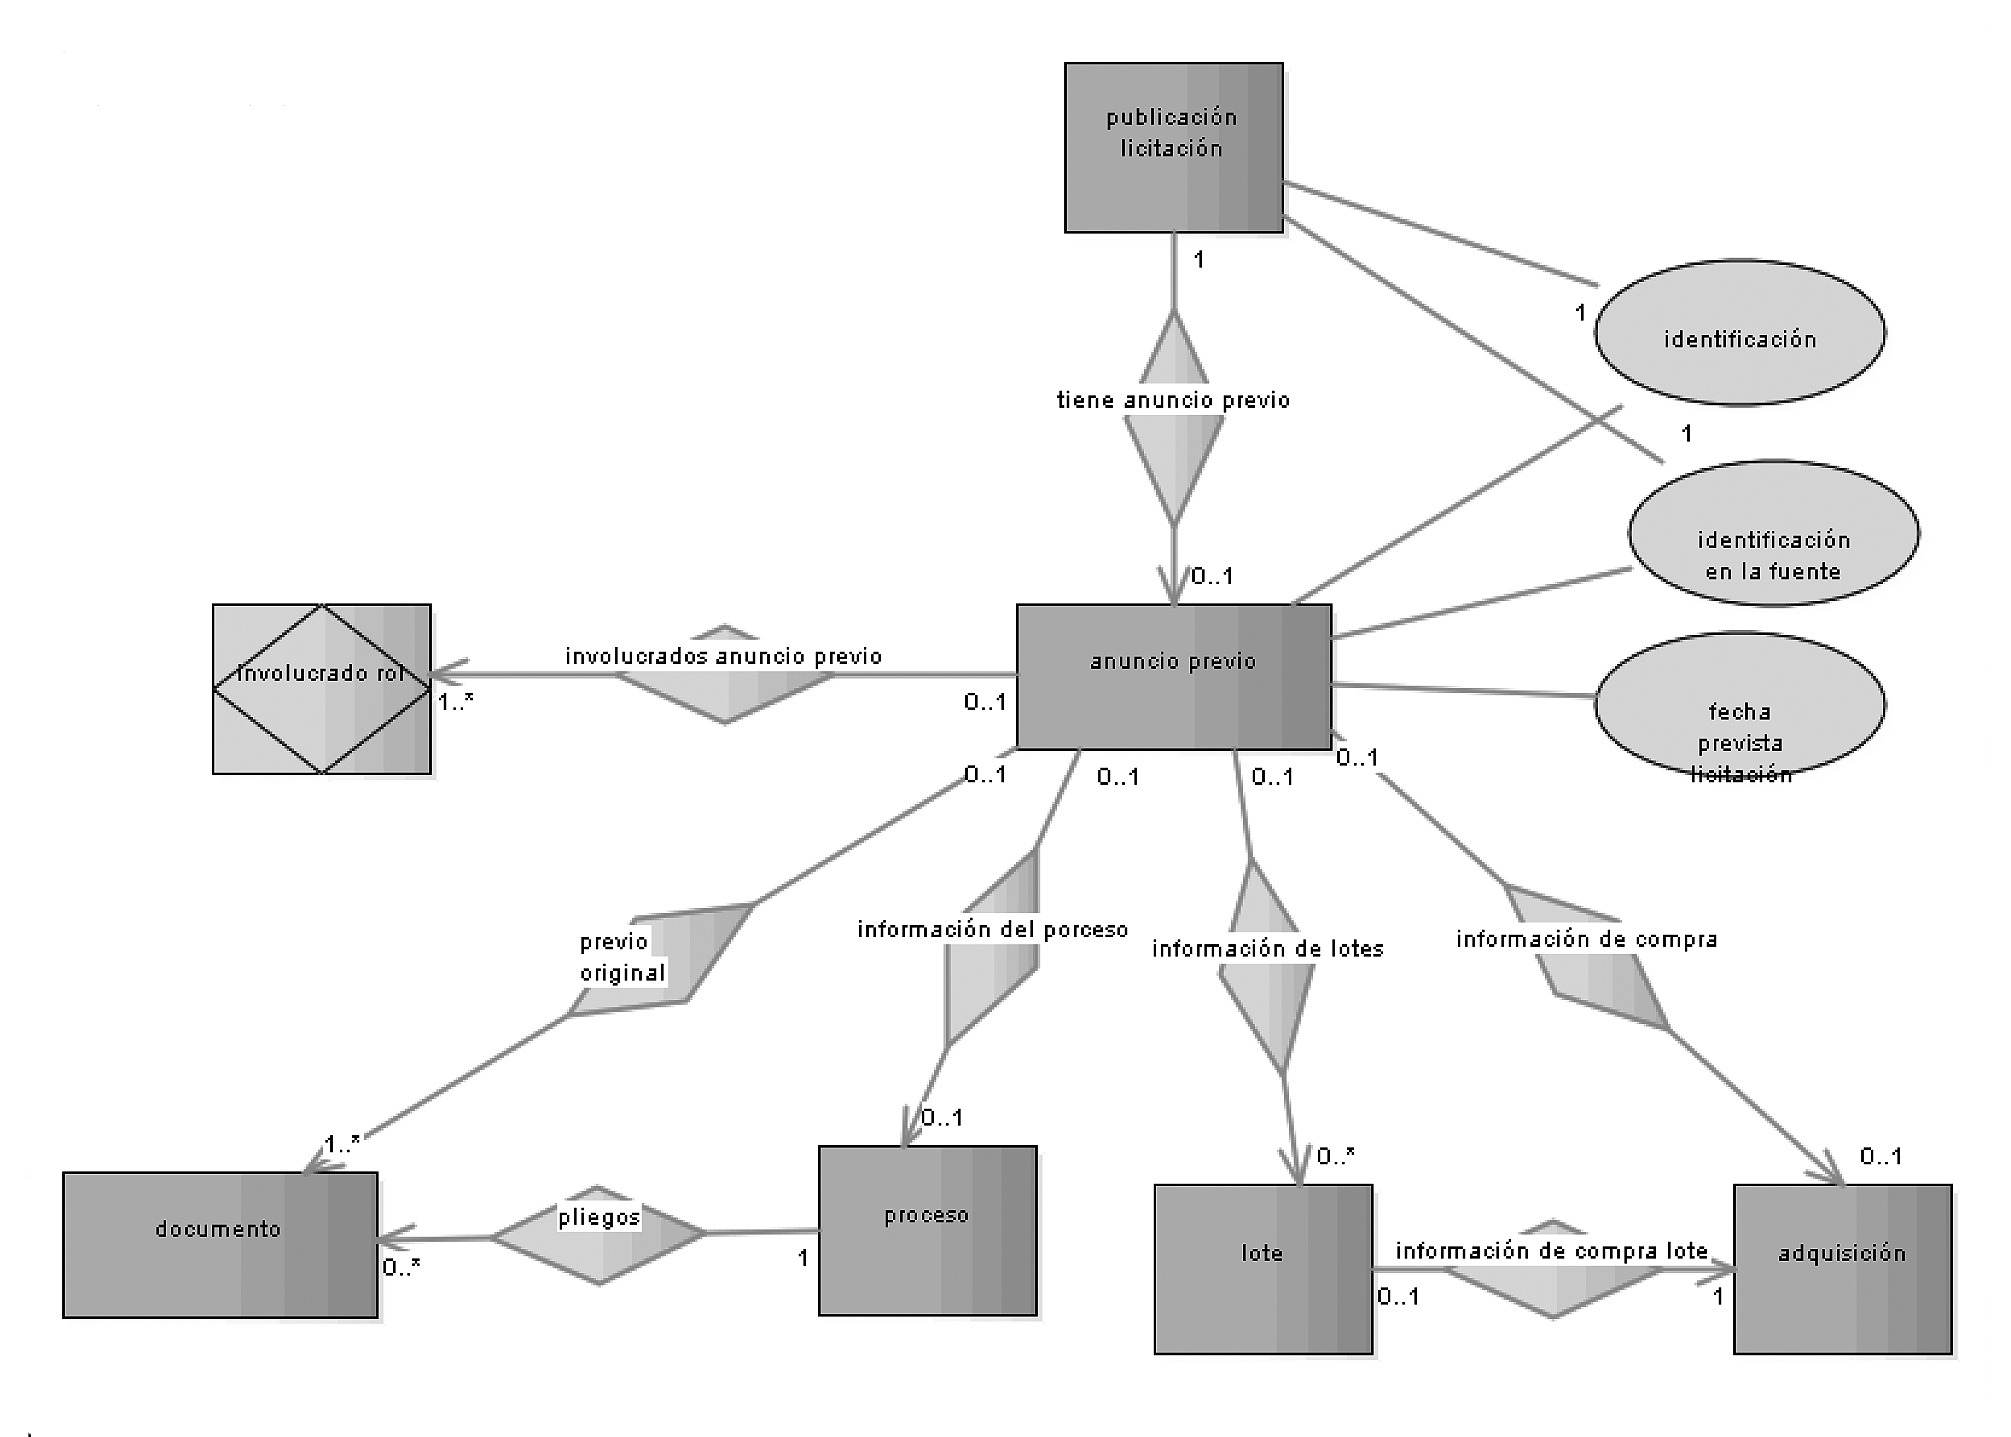
\includegraphics[width=16cm]{images/phd/eproc/10ders-2}
\caption{Modelo de Información de Anuncio Previo de Licitación en opXML.}
\label{fig:10ders-2}
\end{figure}


\begin{figure}[!htb]
\centering
	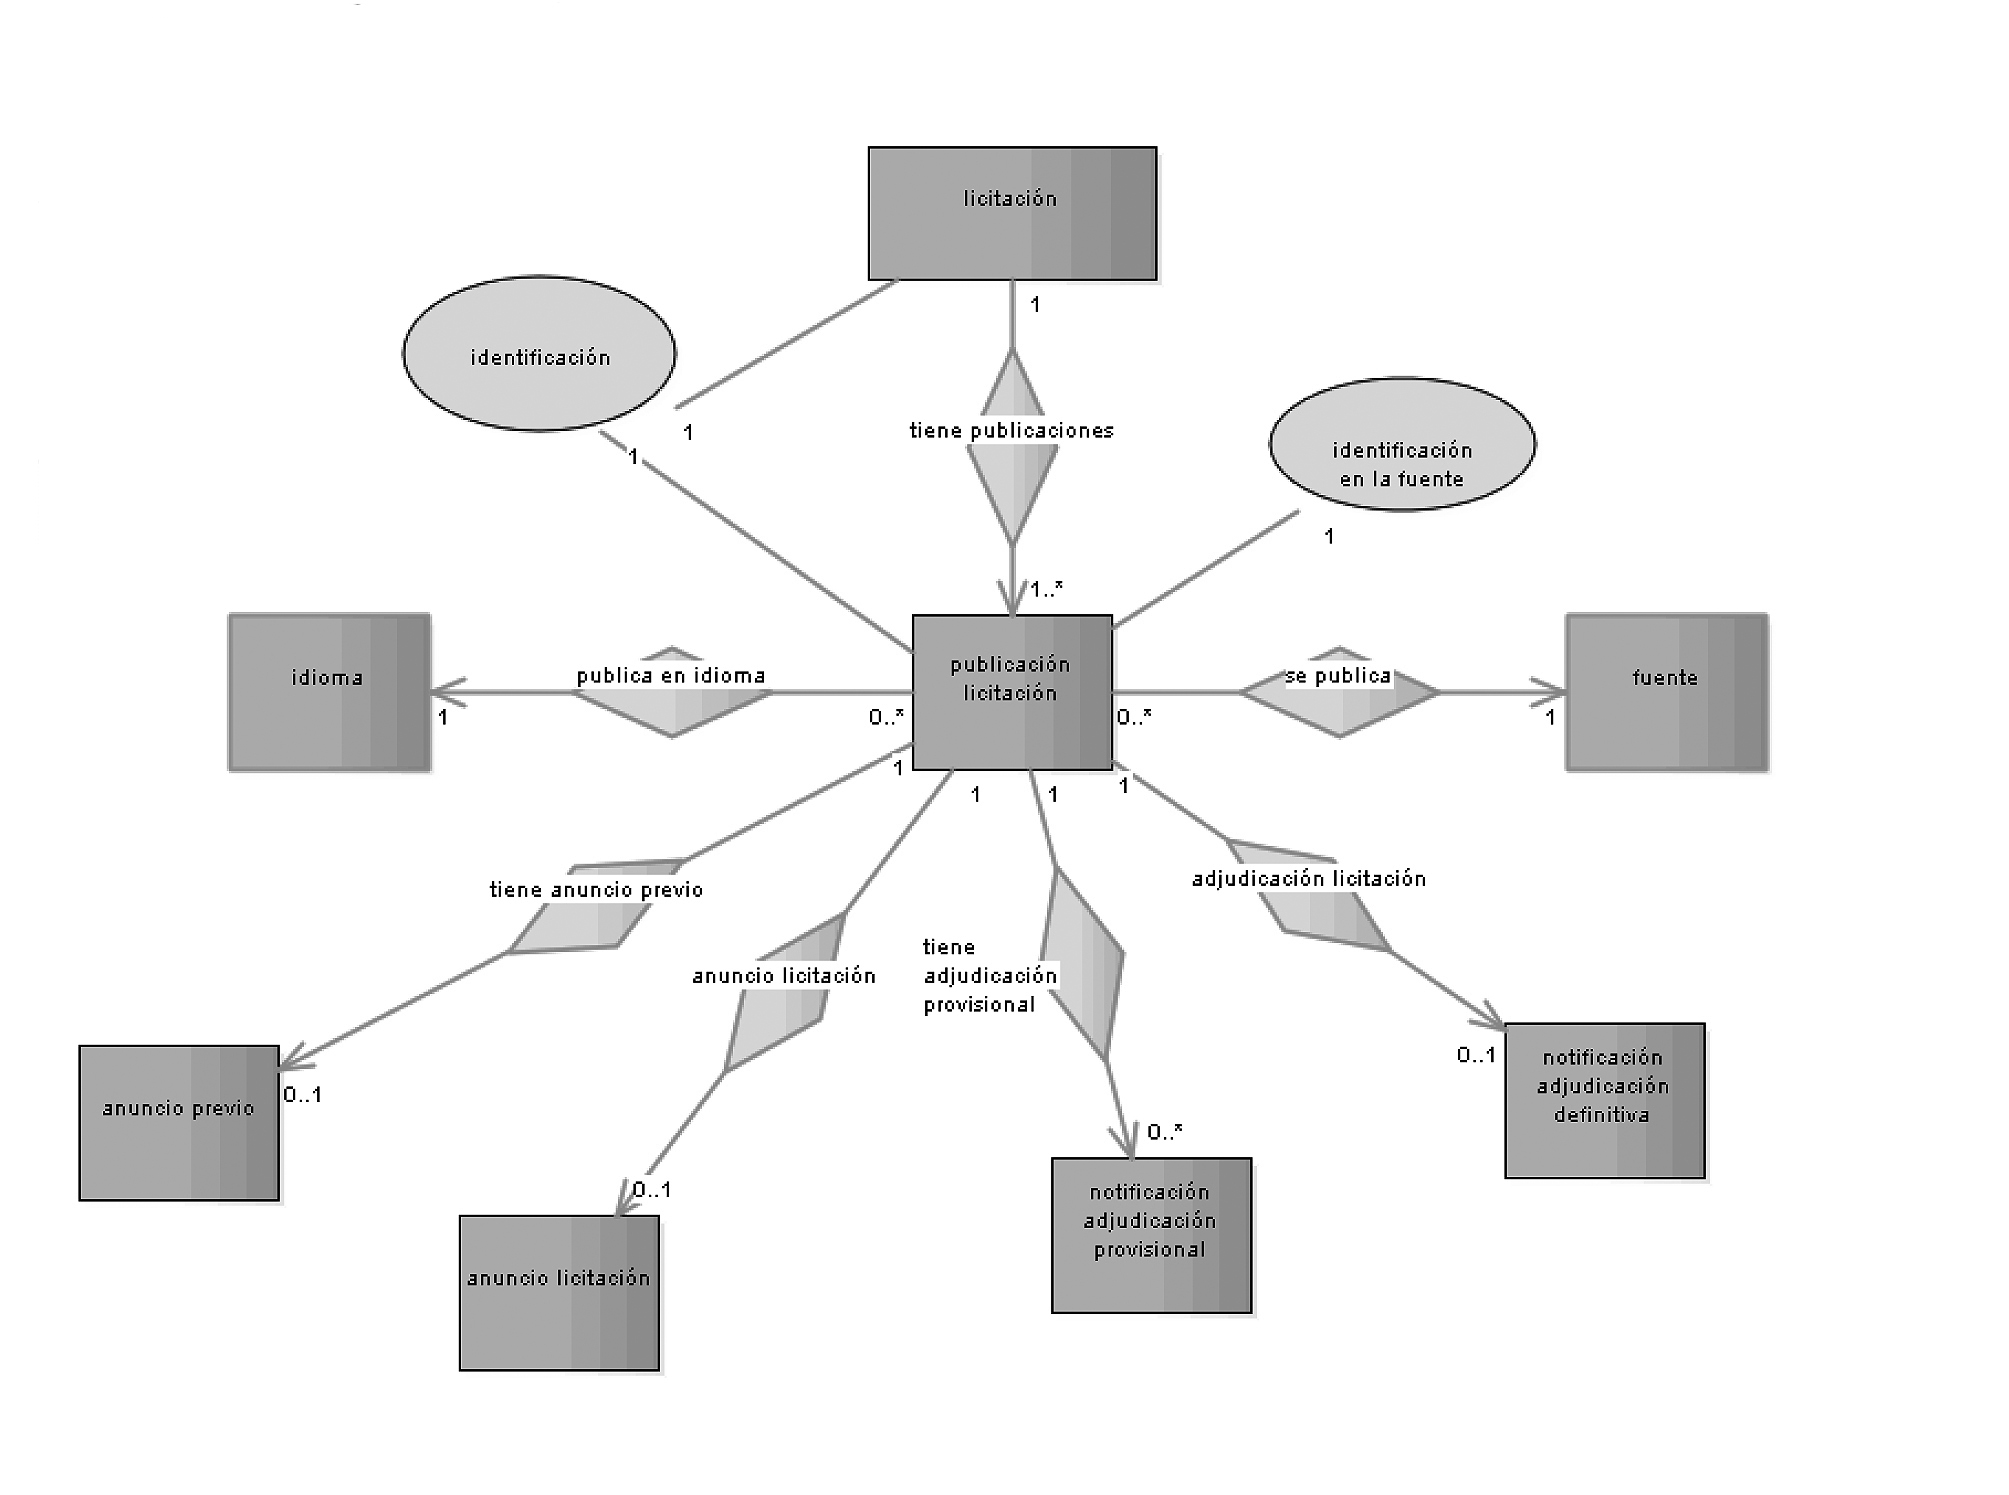
\includegraphics[width=16cm]{images/phd/eproc/10ders-1}
\caption{Modelo de Información de Anuncio de Licitación en opXML.}
\label{fig:10ders-1}
\end{figure}


\begin{figure}[!htb]
\centering
	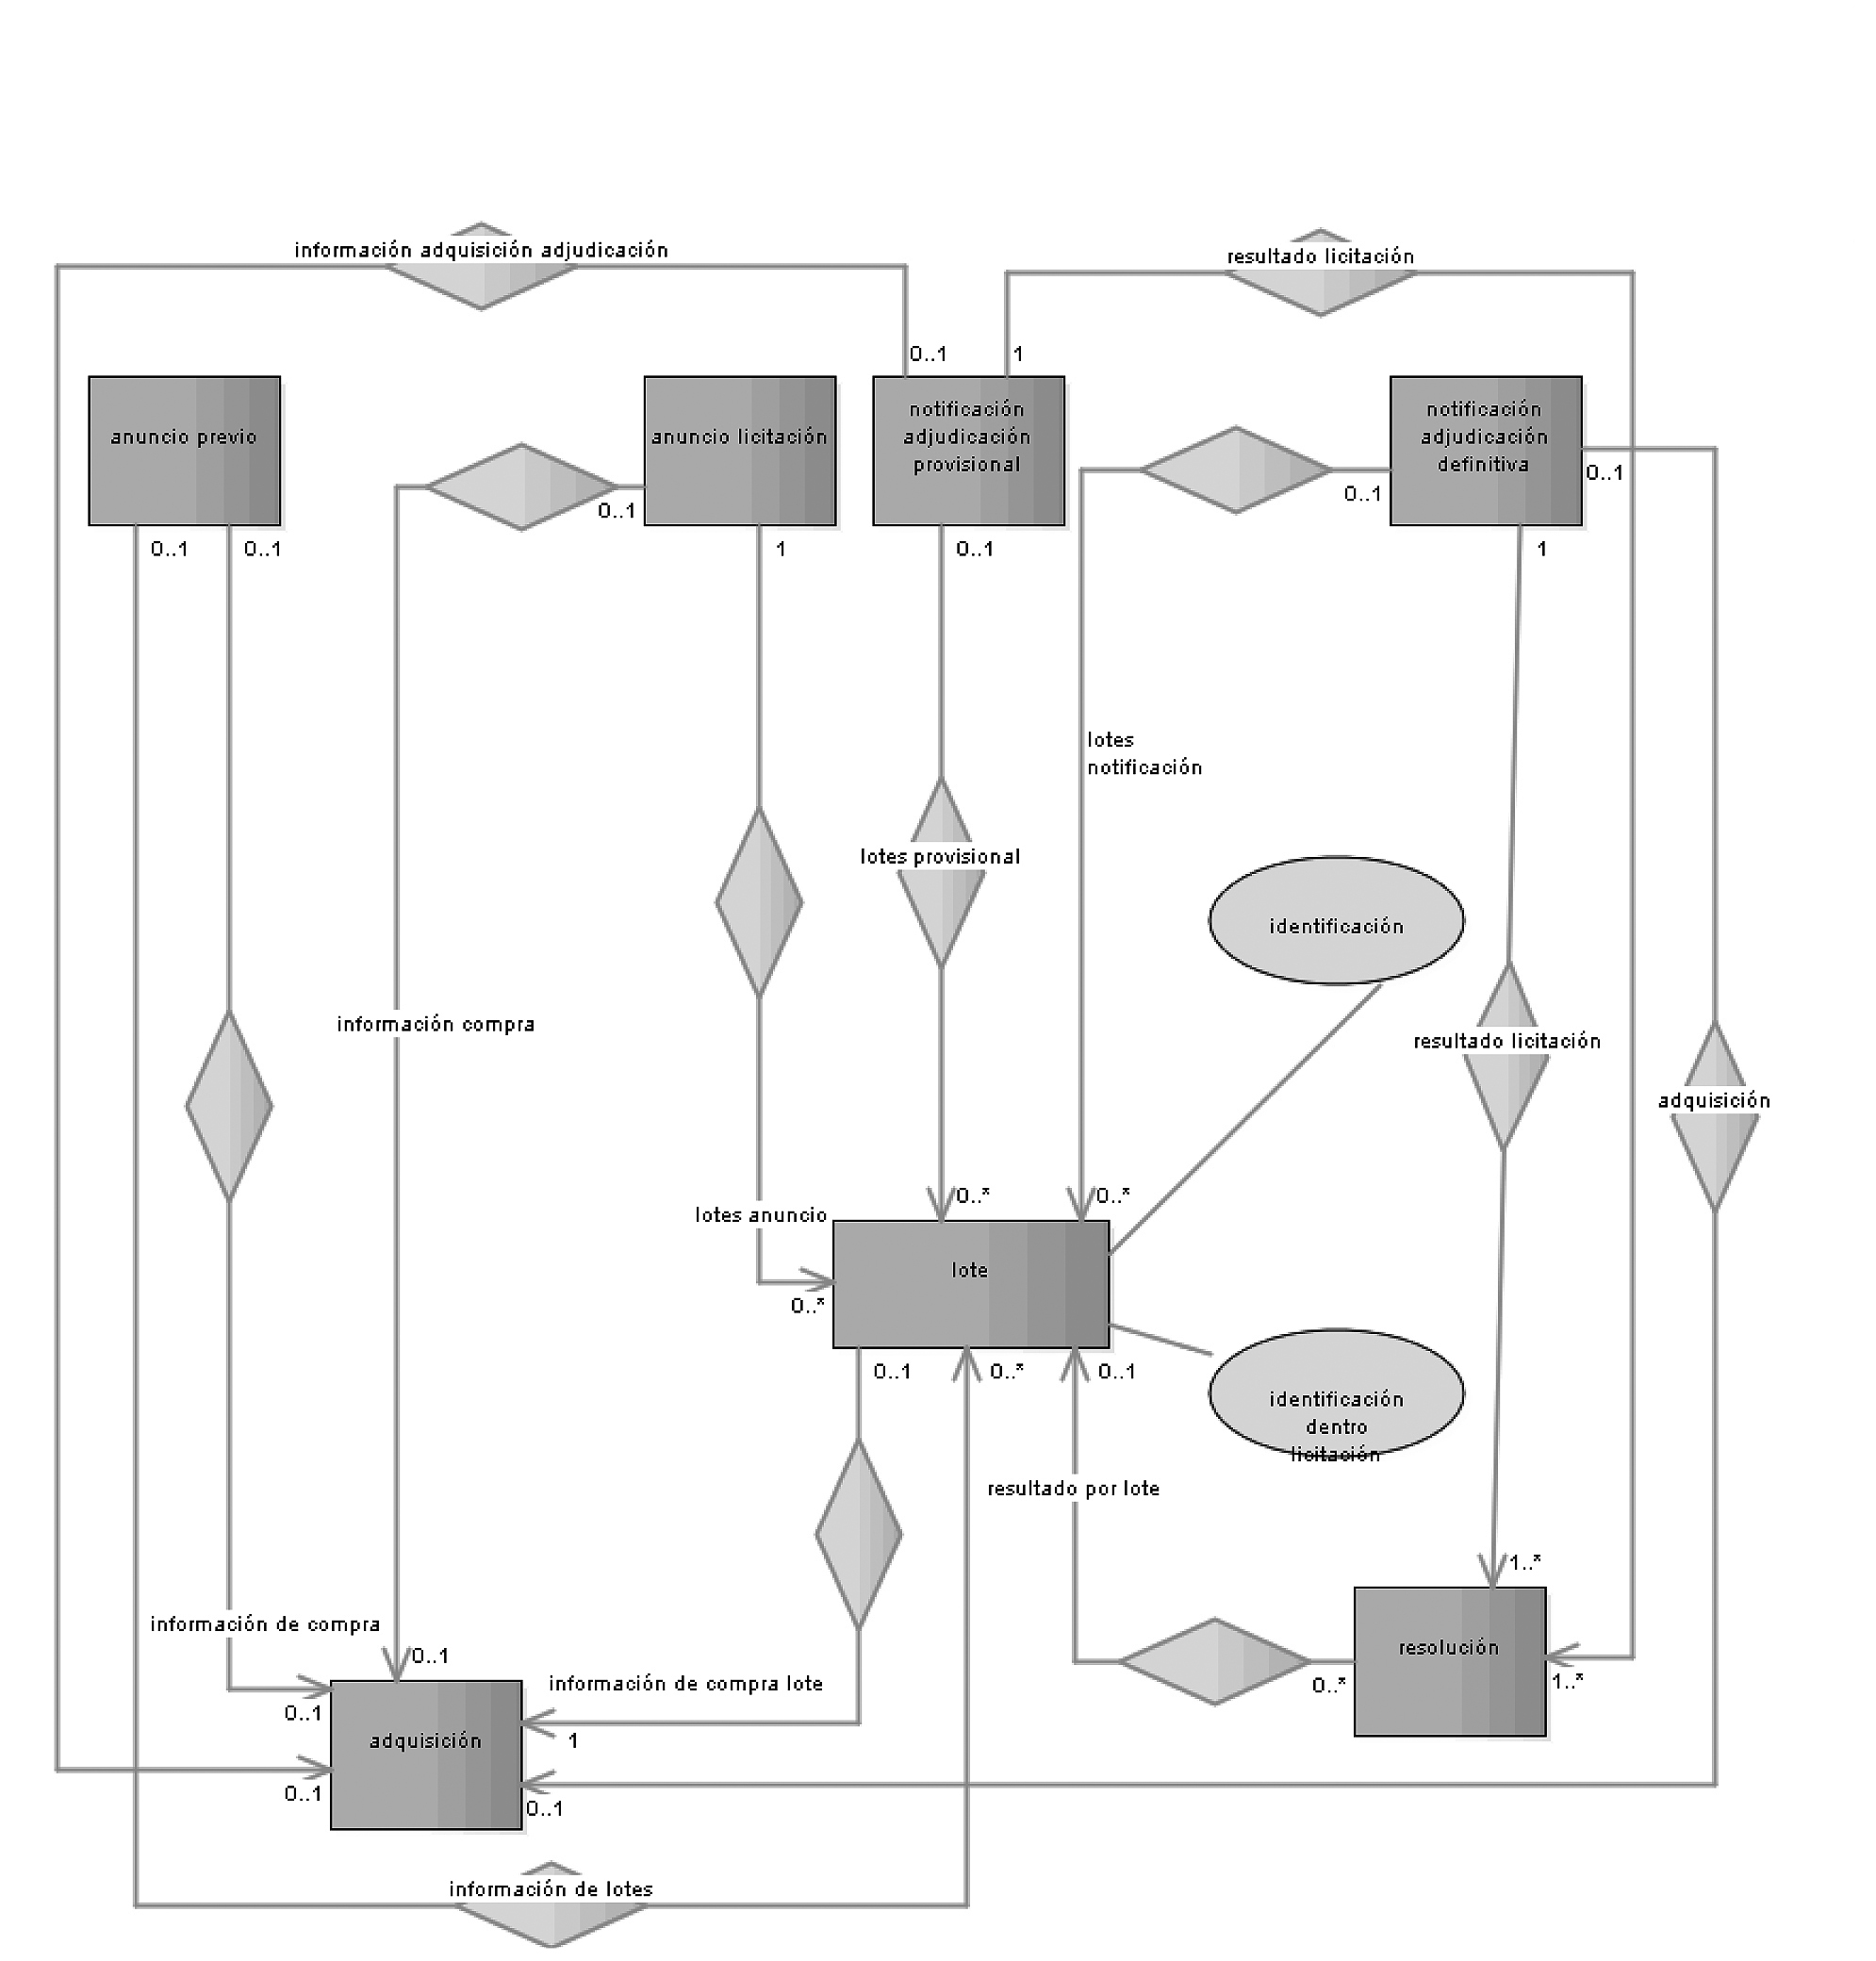
\includegraphics[width=16cm]{images/phd/eproc/10ders-6}
\caption{Modelo de Información de Lote en opXML.}
\label{fig:10ders-6}
\end{figure}

La principal conclusión de esta sección es que se han realizado numerosos y valiosos esfuerzos
para modelar la información disponible en el proceso de contratación pública electrónica, pero
que presentan desventajas en el sentido de una excesiva sobre-especificación, falta de consenso
entre los agentes implicados, etc., que conlleva a una replicación de esfuerzos y a la especificación
de las mismas partes repetidamente. No obstante, todo el conocimiento generado sobre este dominio
debe a largo plazo convertirse en la semilla de algún tipo de estándar que pueda ser aplicado
transversalmente en cualquier entidad con necesidades de contratación de productos y servicios.

\cleardoublepage

\section{Clasificaciones Estándar de Productos}\label{sect:pscs}
Los anuncios de licitación contienen información muy relevante para la búsqueda
de oportunidades de negocio para las distintas empresas. Información sobre la localización,
la cuantía del contrato, la duración, etc., son importantes para concursar
en la adjudicación del contrato. Sin embargo, la información clave en un anuncio
de licitación es el tipo de contrato que se va a adjudicar ya que con ello
se crea el mayor filtro posible para las posibles empresas. En este sentido,
han surgido muchas iniciativas~\cite{Leukel-findings} para aunar la adición de descriptores estándares~\cite{Leukel-standard}
a los anuncios de licitación. A este tipo de información se le denomina
esquemas o catálogos estándar de productos y servicios de forma particular, en general se pueden asimilar 
a un sistema de organización de conocimiento como tesauros, taxonomías o sistemas de clasificación jerárquicos, utilizados
ampliamente para la organización~\cite{Leukel-automating} de grandes colecciones de información como 
documentos, textos, páginas web o recursos multimedia tanto en el ámbito público como privado~\cite{Leukel-comparative}. Estos vocabularios
permiten que los usuarios puedan anotar los objetos de información de una forma
sencilla para que posteriormente su consulta y acceso se simplifique. El uso
de estas técnicas de etiquetado con vocabularios controlados está ampliamente
asentado~\cite{Leukel-ecatalog2005} para describir el ``topic'' de distintos objetos de información, 
suponiendo un primer paso para el tratamiento automático de la información.

Por ejemplo en el contexto europeo han surgido muchas clasificaciones de este tipo
para distintos dominios, disponibles en el servidor de metadatos \gls{RAMON}.
Entre ellos se puede destacar ``the European Schedule of Occupational Diseases'' en el 
campo de la salud, ``the European Education Thesaurus or the European Glossary on Education''
en materia de educación, ``the International Standard Classification of Occupations'' en el ámbito trabajo, etc.
La estructura de estos sistemas de clasificación es similar: jerarquía de entidades y multiling\"{u}ismo, contienen sin embargo, 
factores heterogéneos que impiden su interoperabilidad y que deben ser abordados para conseguir un aprovechamiento eficiente del esfuerzo que supone realizar este tipo
de clasificaciones.

En el campo de la contratación pública electrónica es evidente que este tipo
de paradigmas de clasificación controlada de documentación como anuncios de licitación, lotes,
contratos, etc., es clave para realizar una gestión eficiente de la gran cantidad de información
y documentos que son generados constantemente. Como consecuencia, una de las primeras medidas
impulsadas desde la Comisión Europea ha sido la realización del ``Common Procurement Vocabulary'' (\gls{CPV})~\cite{cpvguide}, se trata de 
una clasificación para describir los objetos de un contrato permitiendo a los agentes
implicados una forma sencilla de buscar los anuncios de licitación. De esta forma, se ha
conseguido armonizar el sistema de codificación de los objetos de contrato. Además, el uso
del CPV es obligatorio desde el 1 de febrero de 2006 según se establece en la directiva 
Regulation (EC) No 2195/2002~\cite{r2195} del Parlamento Europeo. En el ámbito europeo el CPV es, sin duda, 
el vocabulario controlado clave en la esfera de la contratación pública electrónica, que
ha sido fruto del esfuerzo y trabajo desde otras clasificaciones, ver Figura~\ref{fig:evo-cpv}, como la ``Clasificación
Central de Productos'' (\gls{CPC}), la ``Clasificación Industrial Internacional Uniforme'' (\gls{CIIU})
y la ``Clasificación de Productos por Actividades'' (\gls{CPA})

\begin{figure}[!htb]
\centering
	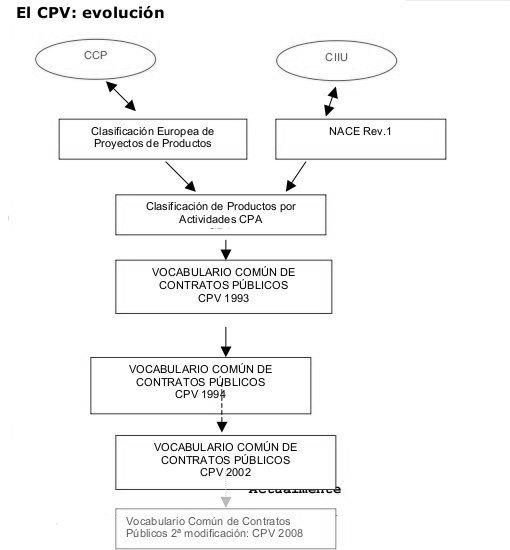
\includegraphics[width=14cm]{images/phd/eproc/evo-cpv}
\caption{Evolución \textit{Common Procurement Vocabulary}.}
\label{fig:evo-cpv}
\end{figure}

Además del CPV existen otras muchas clasificaciones~\cite{Norbert-class} interesantes, ver Tabla~\ref{table:pscs}, en comercio electrónico o bien
para la extracción de estadísticas, que han sido formuladas por diferentes organismos como
la \gls{UNESCO}, \gls{ONU} o el Gobierno de Estados Unidos, que actualmente tienen en el mejor de los casos \textit{mapeos} entre ellas, 
pero cuyo acceso suele ser complicado tanto por los formatos en los que se presentan, habitualmente MSExcel o \gls{PDF}, como por 
las aplicaciones y sistemas de búsqueda muy rígidos. 

\begin{longtable}[c]{|p{6cm}|l|p{6cm}|} 
\hline
  \textbf{Clasificación} &  \textbf{Acrónimo} & \textbf{Organismo} \\\hline
\endhead
\textit{Combined Nomenclature} 2012 (desde 1995) & \gls{CN} & Unión Europea  \\ \hline
\textit{Central Product Classification}, version 2 (2008) & \gls{CPC} & Unión Europea \\ \hline
Clasificación de Productos por Actividad (2008) & \gls{CPA} & Unión Europea \\ \hline
\textit{Integrated Tariff of the European Communities)} & \gls{TARIC} & Unión Europea\\ \hline
\textit{International Standard Industrial Classification of All Economic Activities, Rev.4} & \gls{ISIC} & \textit{United Nations Statistics Division} \\ \hline
\textit{North American Product Classification System} & \gls{NAPCS} & Agencias estadísticas de Canadá, México y Estados Unidos\\ \hline
\textit{North American Industry Classification System} 2007 y 2012 & \gls{NAICS} & Gobierno de Estados Unidos \\ \hline
\textit{PRODuction COMmunautaire} & \gls{PRODCOM} & Unión Europea \\ \hline
\textit{Standard International Trade Classification, Revision 4} & \gls{SITC} & \textit{United Nations Statistics Division} \\ \hline
\textit{Nomenclature générale des activités économiques dans les Communautés européennes} & \gls{NACE} & Unión Europea \\ \hline
\textit{United Nations Standard Products and Services Code} & \gls{UNSPSC} & Consorcio entre ellos la ONU\\ \hline
  \multicolumn{3}{|c|}{\ldots}  \\ \hline
\hline
\caption{Catálogo de Clasificaciones Estándar de Productos.}\label{table:pscs}\\    
\end{longtable}

El uso de estas clasificaciones es clave para la trazabilidad de proveedores de productos y servicios,
sistemas de anotación y etiquetado, extracción de información, etc. En el contexto de los anuncios
de licitación representan el método de especificar el objeto del contrato pero no todo
son ventajas, ya que al existir una amplia variedad, es difícil mantener la consistencia entre ellas
y sus distintas versiones, forzando a que se dupliquen esfuerzos en los distintos organismos para 
extraer información basada en estos códigos. 

\section{Información sobre Organizaciones}
\textit{An organization is considered to be a set of constraints on the activities performed by agents}. 

Este enfoque de organización fue presentando por Max Weber~\cite{Weber1978}, posteriormente Mintzberg realizó un análisis
de las estructuras organizacionales distinguiendo entre cinco tipos y configuraciones diferentes. Estos enfoques
ponen de manifiesto los mecanismos que operan dentro de las organizaciones con el objetivo
de coordinarse para conseguir un determinado objetivo materializado a través de diferentes metas,
procesos y reglas de negocio, posición en el mercado y comunicación. Existen trabajos~\cite{Fox95anorganisation}
en los cuales se intenta modelar la estructura de una organización, pero que no ha abordado problemas como:
1) falta de información para definir el \textit{status} de una organización, 2) maraña de subdivisiones
para especificar la estructura entre los elementos de la organización, 3) ausencia de capacidades léxicas
para describir los conceptos y relaciones que se manejan en una organización, 4) distintos tipos
de nombrado, etc. 

La problemática para definir la estructura de una organización y su actividad no es sencilla, ya que puede
ser muy diversa dependiendo de su organización, objetivos particulares, etc., es por ello que en el campo
de la contratación pública electrónica resulta de gran valor la posibilidad de disponer de la información
de los agentes implicados en el proceso administrativo, para así poder trazar su actividad a lo largo
del tiempo. Desde un punto de vista del órgano contratante, su perfil debe estar disponible al público. Este
perfil además de los anuncios de licitación debe comprender información de contacto, persona encargada, etc., 
toda esta información actualmente está accesible pero de una forma ligeramente rudimentaria. De igual forma, cuando
los contratos son adjudicados, se dispone de la información relativa a la empresa adjudicataria pero de nuevo
el acceso a esta información sigue un modelo tradicional. Un proceso lógico sería que una entidad especificara
su perfil de contrante siguiendo un estándar en cuanto a su organización interna y que por otro lado
las empresas pudieran definir un perfil en el cual indicar sus intereses y así facilitar el proceso de 
encaje entre tipos de contrato e intereses. 

\section{Evaluación del estado actual del mundo de e-Procurement}
En este capítulo se han repasado los conceptos clave sobre contratación
pública y en concreto la contratación pública electrónica. Desde la
Unión Europea existe un claro compromiso y liderazgo por impulsar este proceso
administrativo por la relevancia y el impacto que tiene en la sociedad, ya que sin lugar a dudas las cifras de inversión y gasto que se manejan
resultan de gran interés para las empresas de todo tipo y sector. Sin embargo, aunque las distintas iniciativas han conseguido avanzar en la 
consecución de este gran reto, existen puntos clave en los cuales las soluciones existentes no han
conseguido desarrollar toda su capacidad para atraer a las empresas
y así conseguir un mercado competitivo a nivel paneuropeo. En este sentido,
la disponibilidad de soluciones técnicas ya existentes así como las que
se están desarrollando y la transferencia tecnológica desde los entornos
académicos deben mejorar las fases de \eproc. Esta inversión
en nuevas capacidades es clave para la adopción y uso efectivo de este proceso administrativo
de forma electrónica. Por ello, tanto la publicación como la accesibilidad transfronteriza
a la información y sistemas de contratación pública electrónica es clave. 

Los retos que se plantean son diversos y abarcan desde la generación de confianza suficiente
entre entidades adjudicadoras y proveedores a través de un marco legislativo adecuado, hasta
la generación de herramientas y medios que permitan la comunicación efectiva entre los distintos
agentes participantes en el proceso. Muchas veces, los requisitos técnicos en lugar de facilitar
la adopción, suponen una gran barrera de entrada, un simple sistema de autenticación se puede
convertir en un gran inconveniente para el uso de los medios electrónicos. No obstante,
la transición hacia este nuevo mundo electrónico para la contratación se está realizando
de forma sostenible y a distintas velocidades, dependiendo de las capacidades de las propias
Administraciones. Las prioridades para realizar el despliegue definitivo se centran en el uso
de medidas incentivadores o penalizadoras para acelerar este nuevo método, impulsar
la participación paneuropea en los distintos procesos de licitación pública, simplificando 
las condiciones a satisfacer para el uso de los nuevos sistemas y facilitando la autenticación
entre los distintos agentes económicos. Finalmente, todos estos retos y prioridades se realizarán
bajo una base normalizada, tanto en tecnología como en estándares, para la distinta documentación
generada durante el proceso con el objetivo final de que paulatinamente todo tipo de empresas
puedan competir por los contratos públicos bajo las mismas condiciones con las consiguientes
ventajas para el mercado económico común.


% \section{Modelos Conceptuales de Dominio}\label{sect:mcds}
% 



% 
% 
% \begin{figure}[!htb]
% \centering
% 	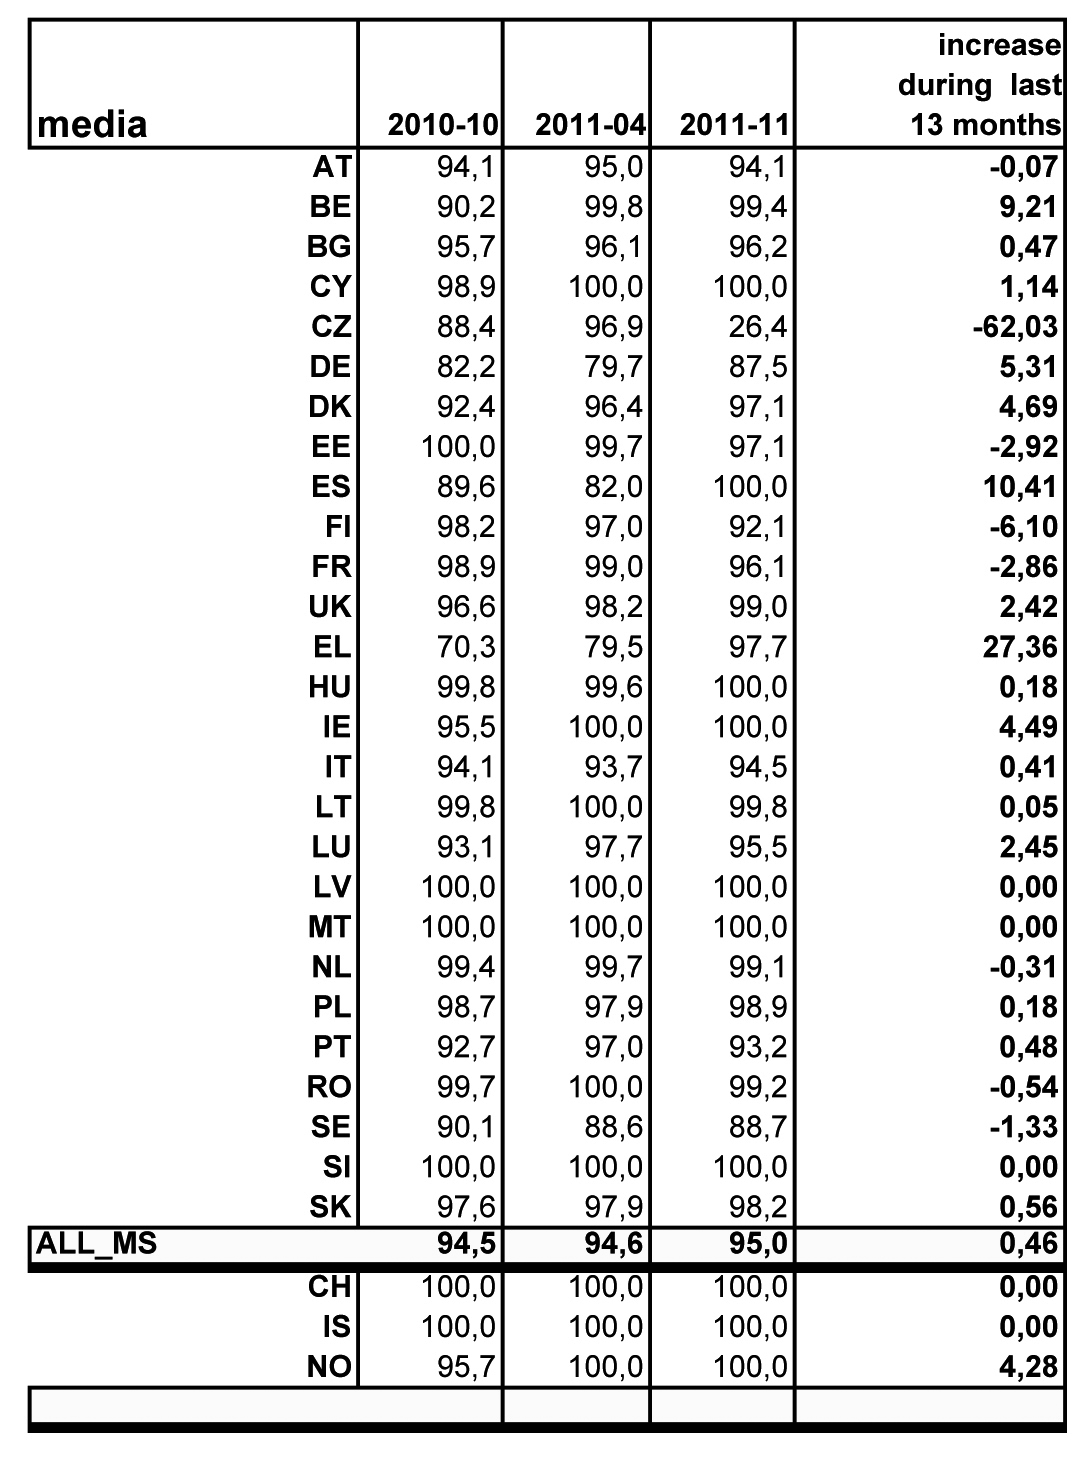
\includegraphics[width=10cm]{images/phd/eproc/circa-2}
% \caption{Porcentaje y Tipo de Publicación de Anuncios de Licitación en TED (2).}
% \label{fig:circa-1}
% \end{figure}
% 
% 


% 
% \begin{figure}[!htb]
% \centering
% 	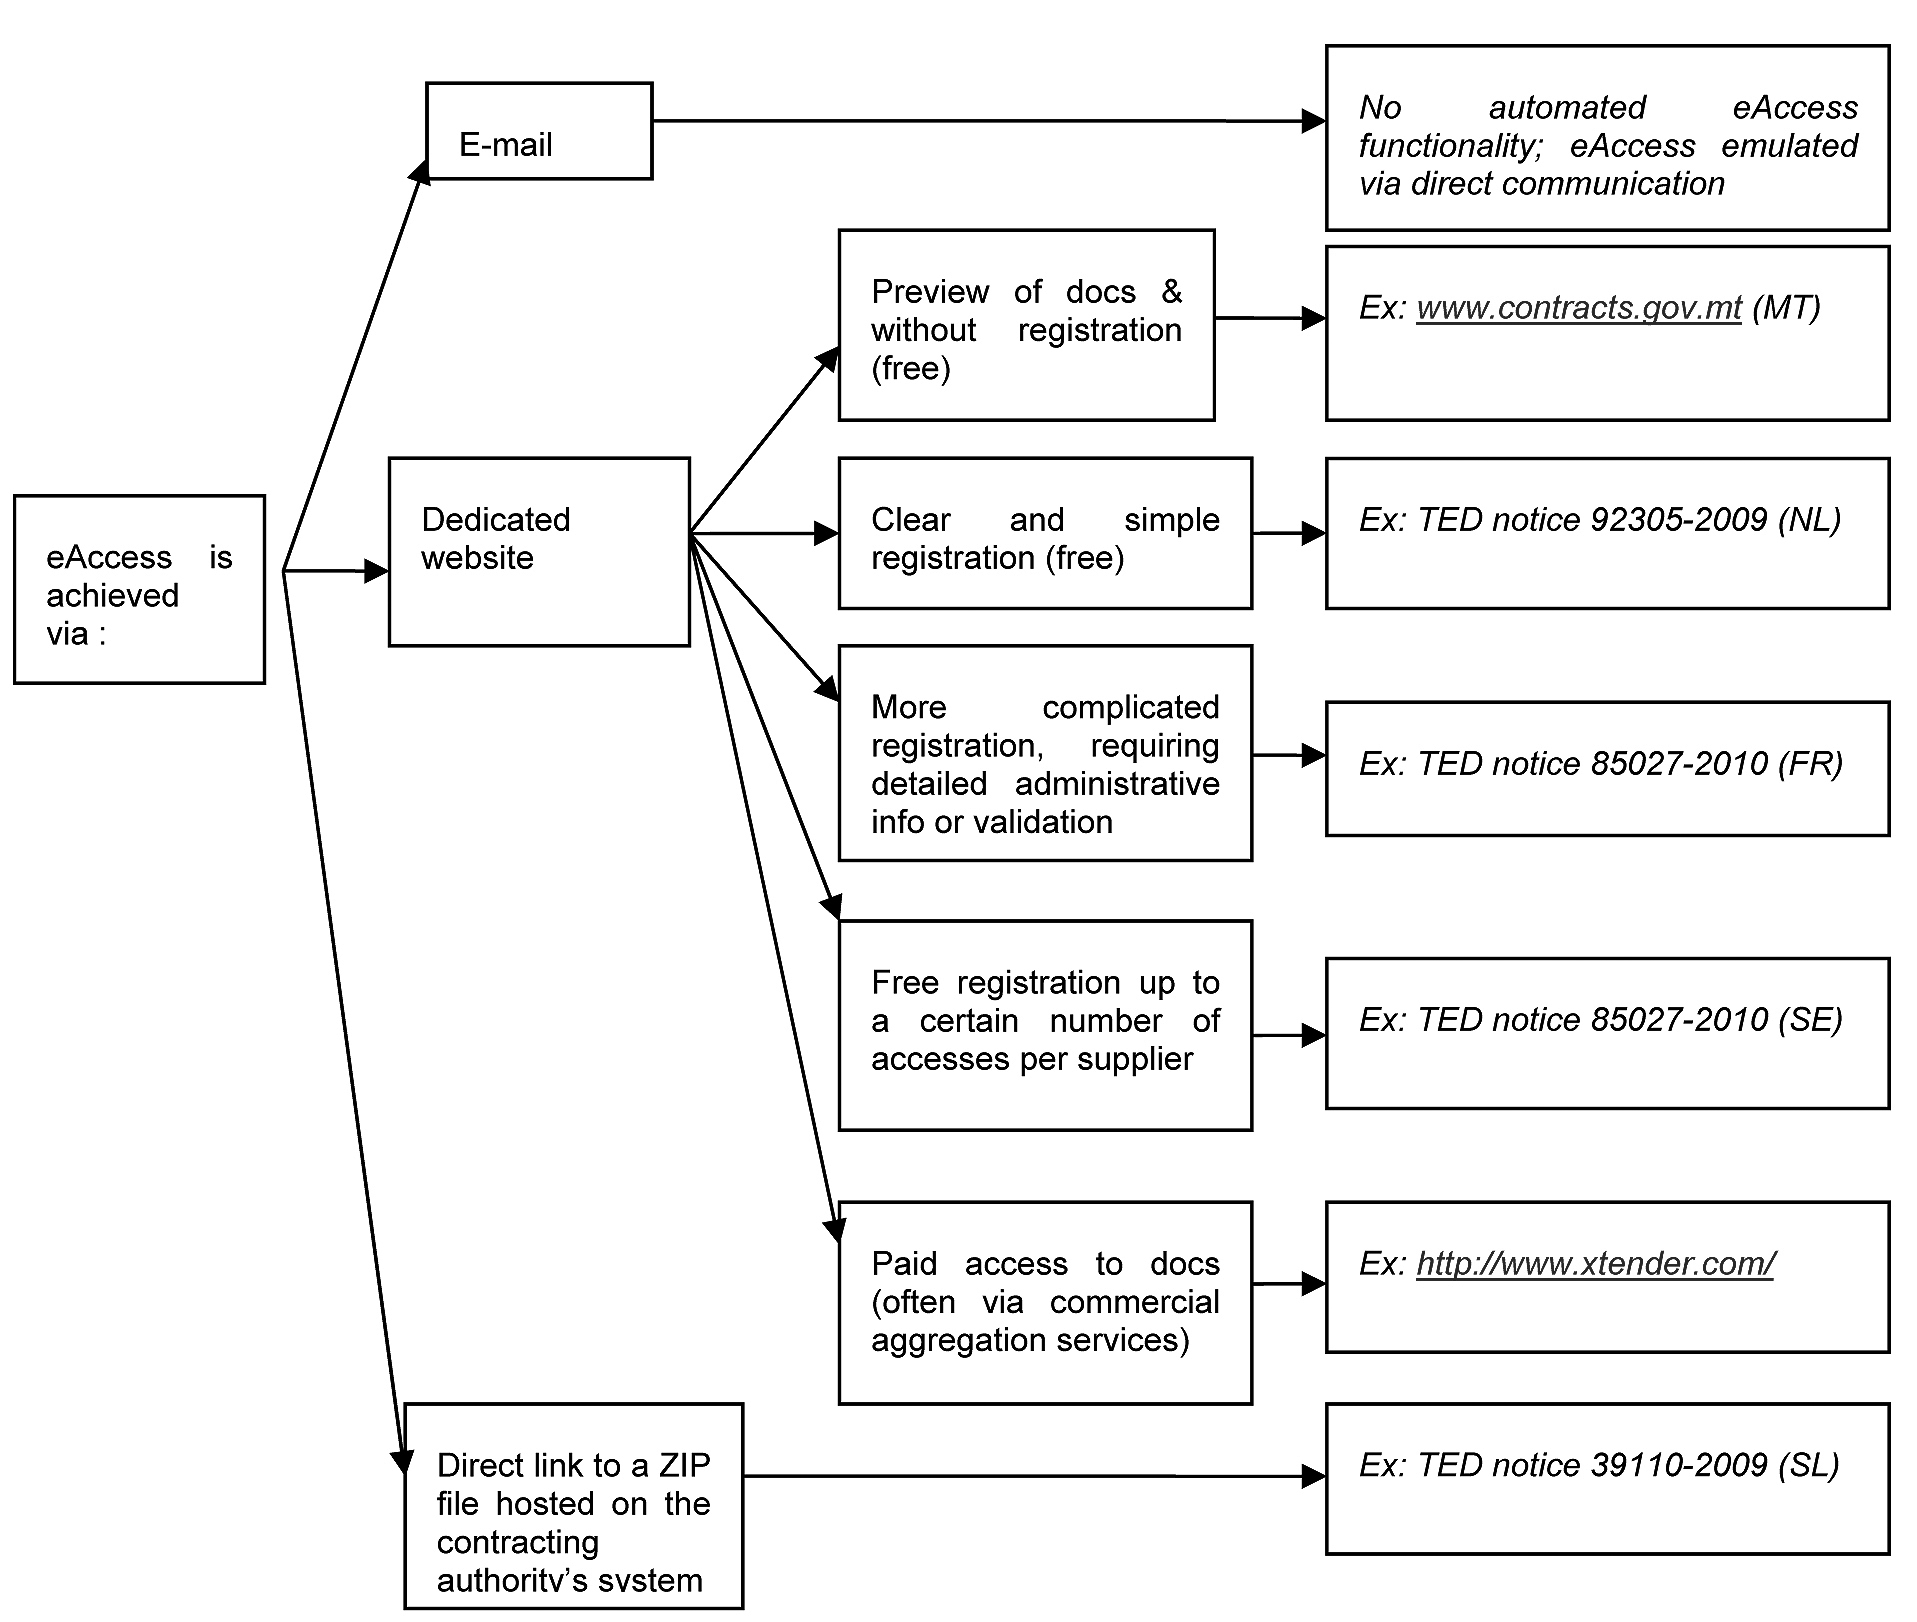
\includegraphics[width=10cm]{images/phd/eproc/ted-4}
% \caption{Características en \textit{eAccess} de la Unión Europea por Siemens.}
% \label{fig:ted-4}
% \end{figure}
% 
% 
% 
% \begin{figure}[!htb]
% \centering
% 	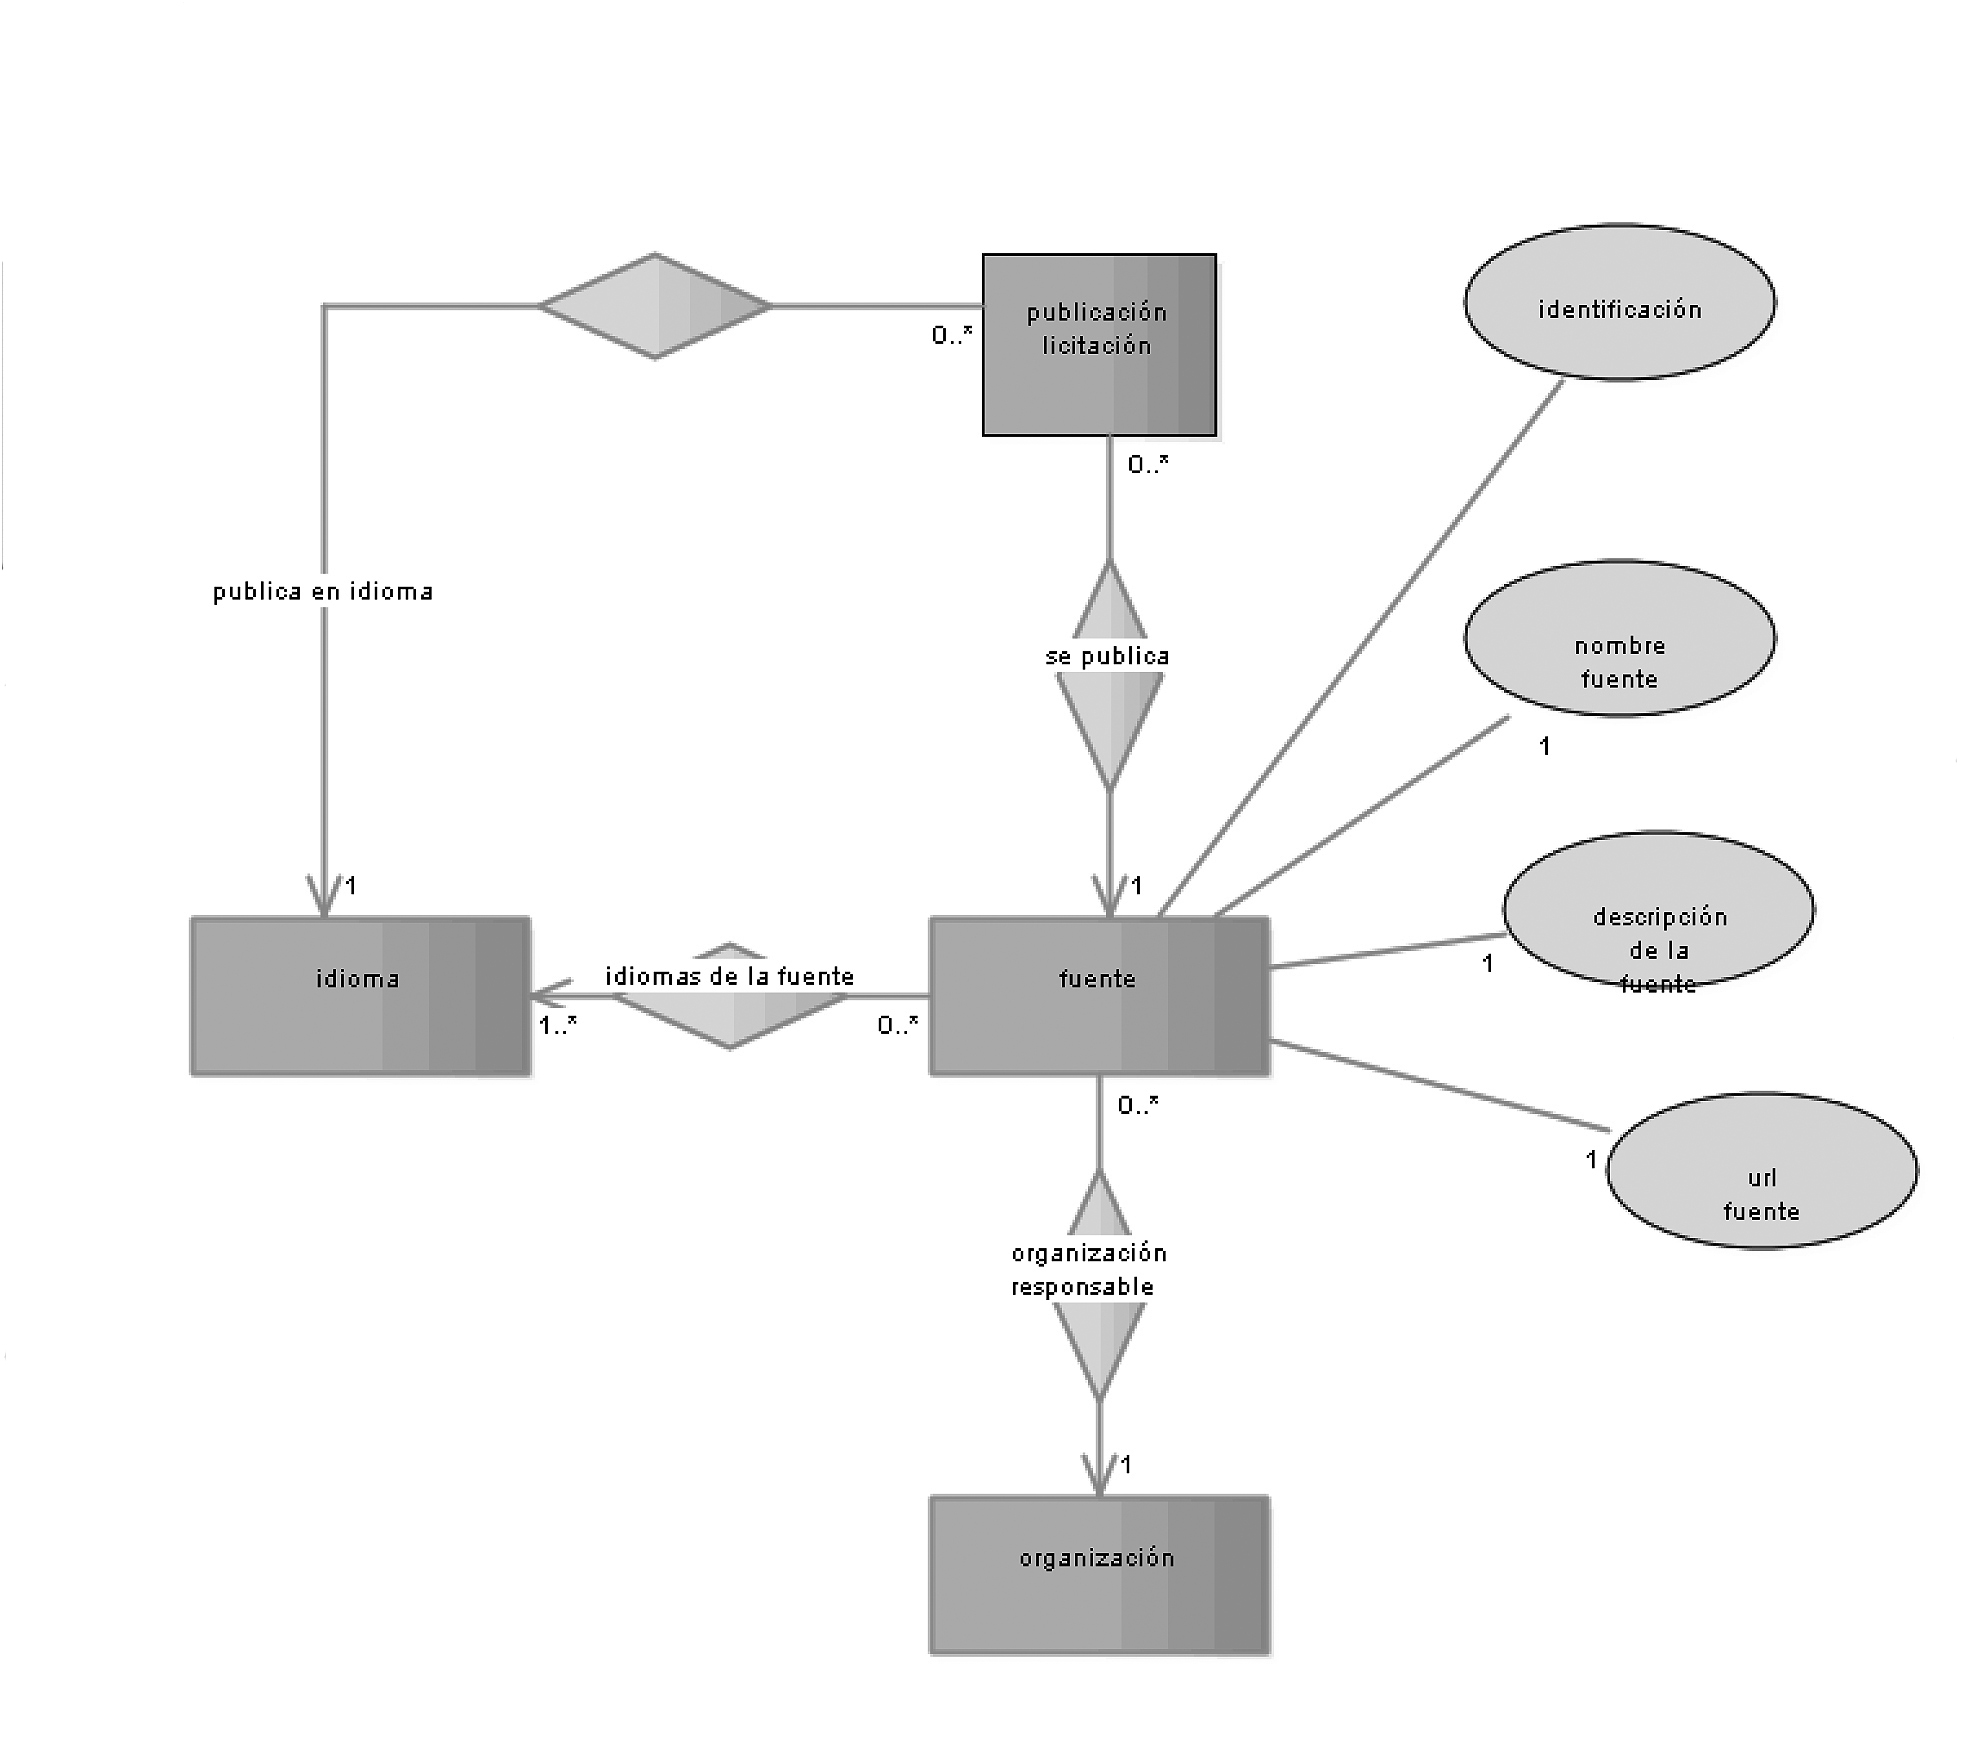
\includegraphics[width=10cm]{images/phd/eproc/10ders-8}
% \caption{Fuente de Publicación en el proyecto 10ders.}
% \label{fig:10ders-8}
% \end{figure}
% 
% \begin{figure}[!htb]
% \centering
% 	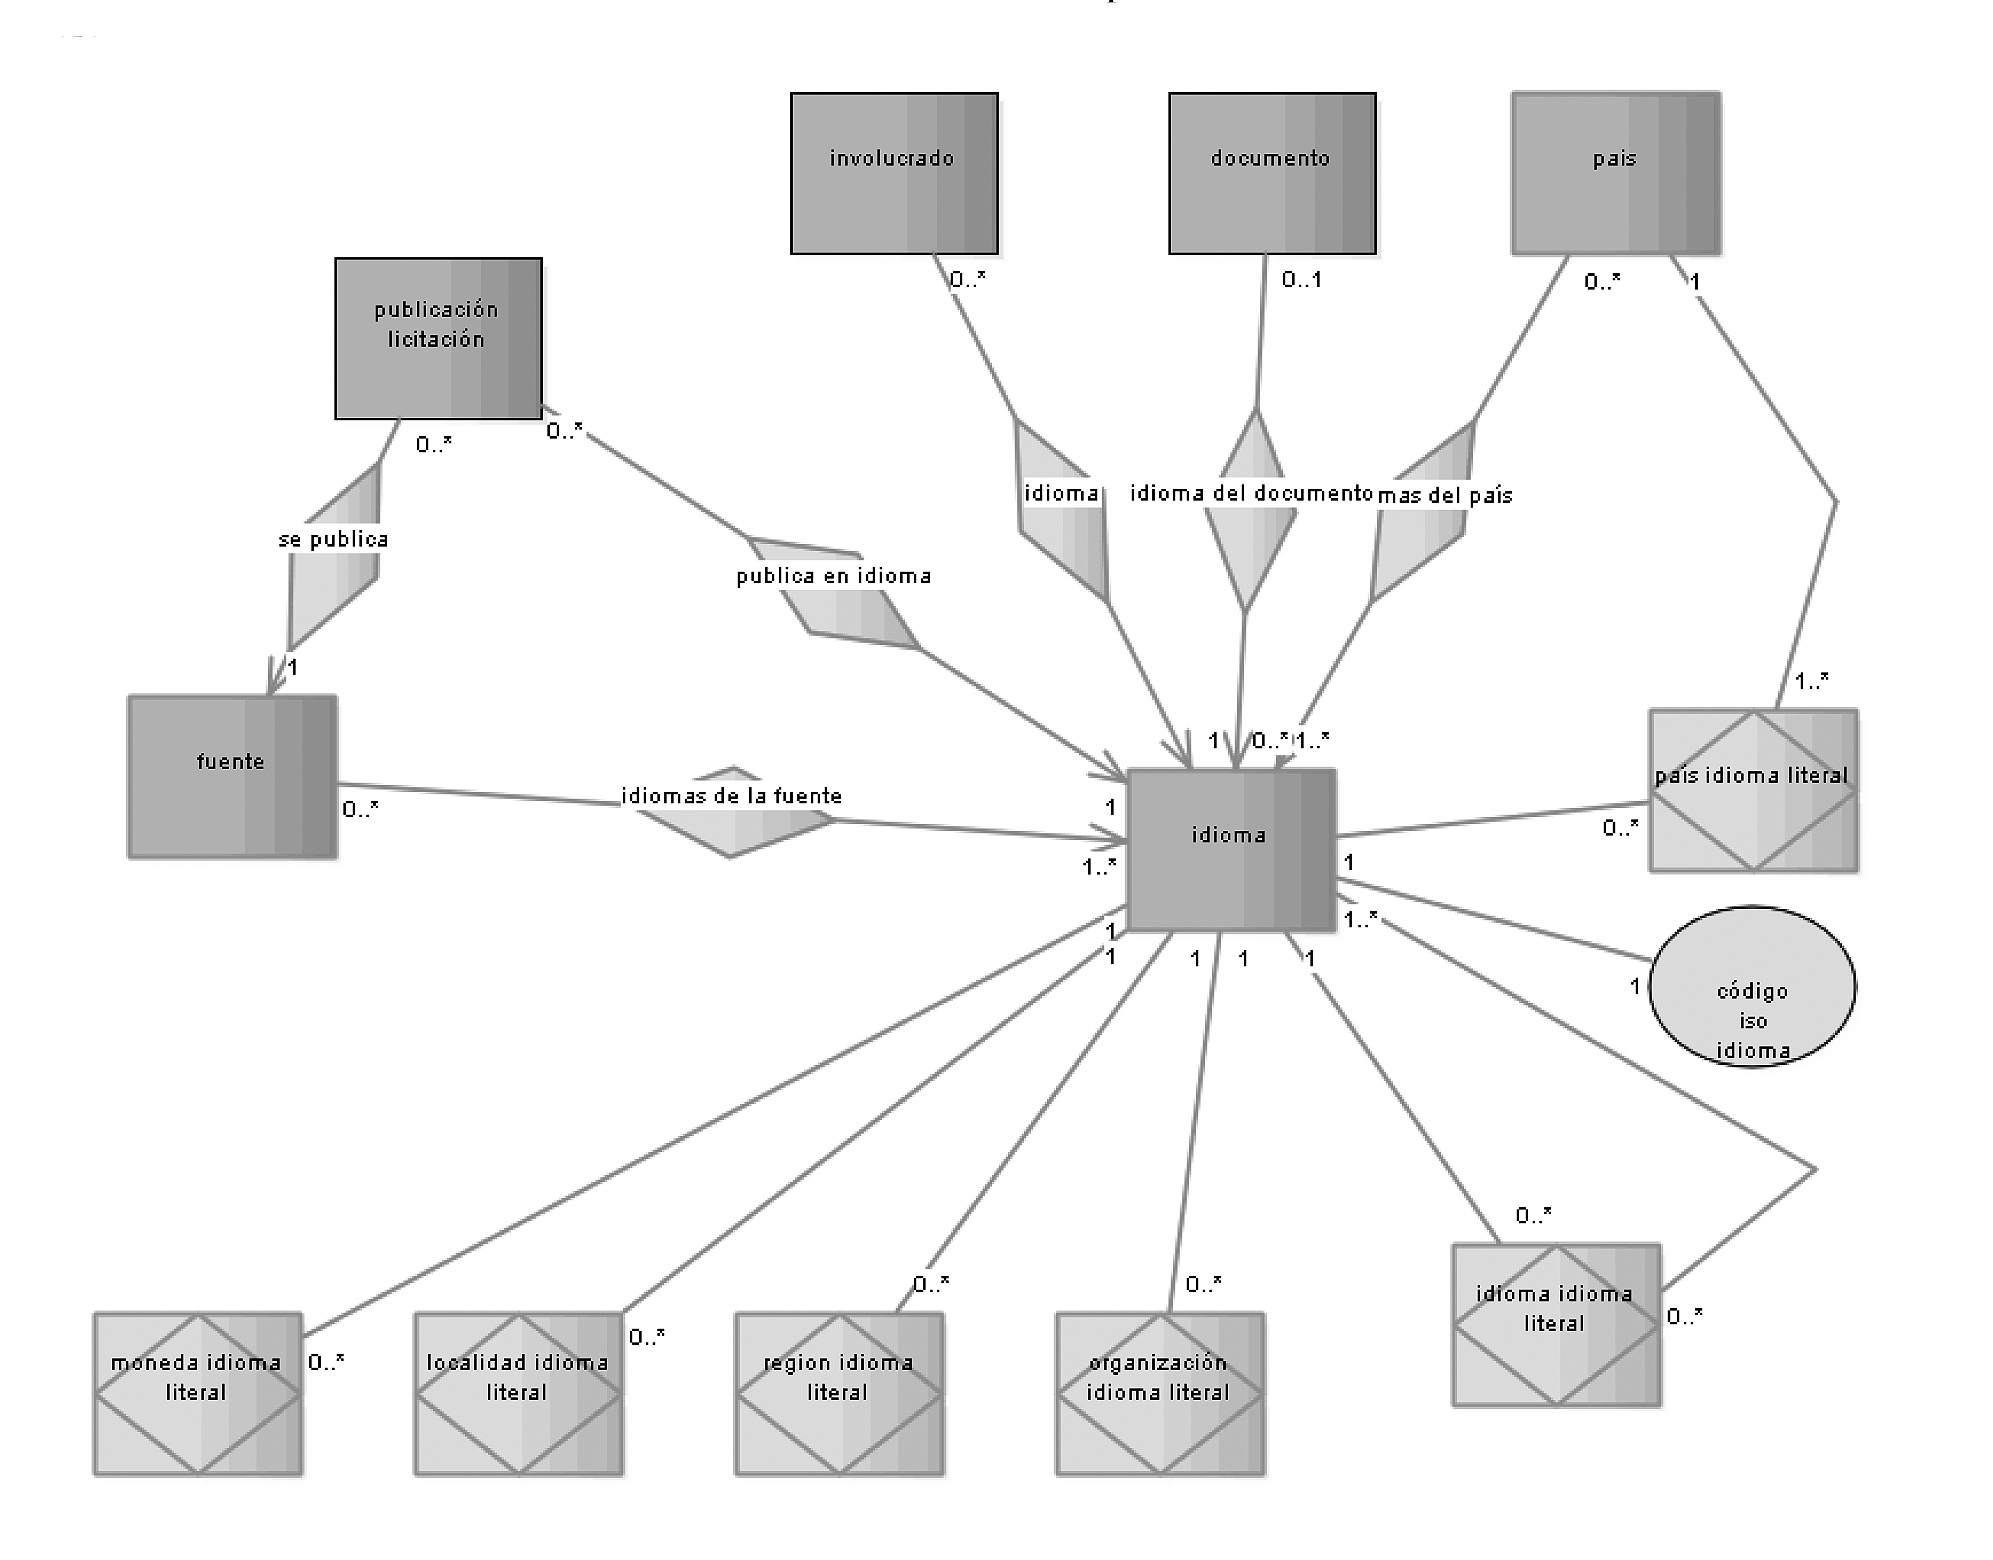
\includegraphics[width=10cm]{images/phd/eproc/10ders-9}
% \caption{Idioma en el proyecto 10ders.}
% \label{fig:10ders-9}
% \end{figure}
% 
% 
% 
% \begin{figure}[!htb]
% \centering
% 	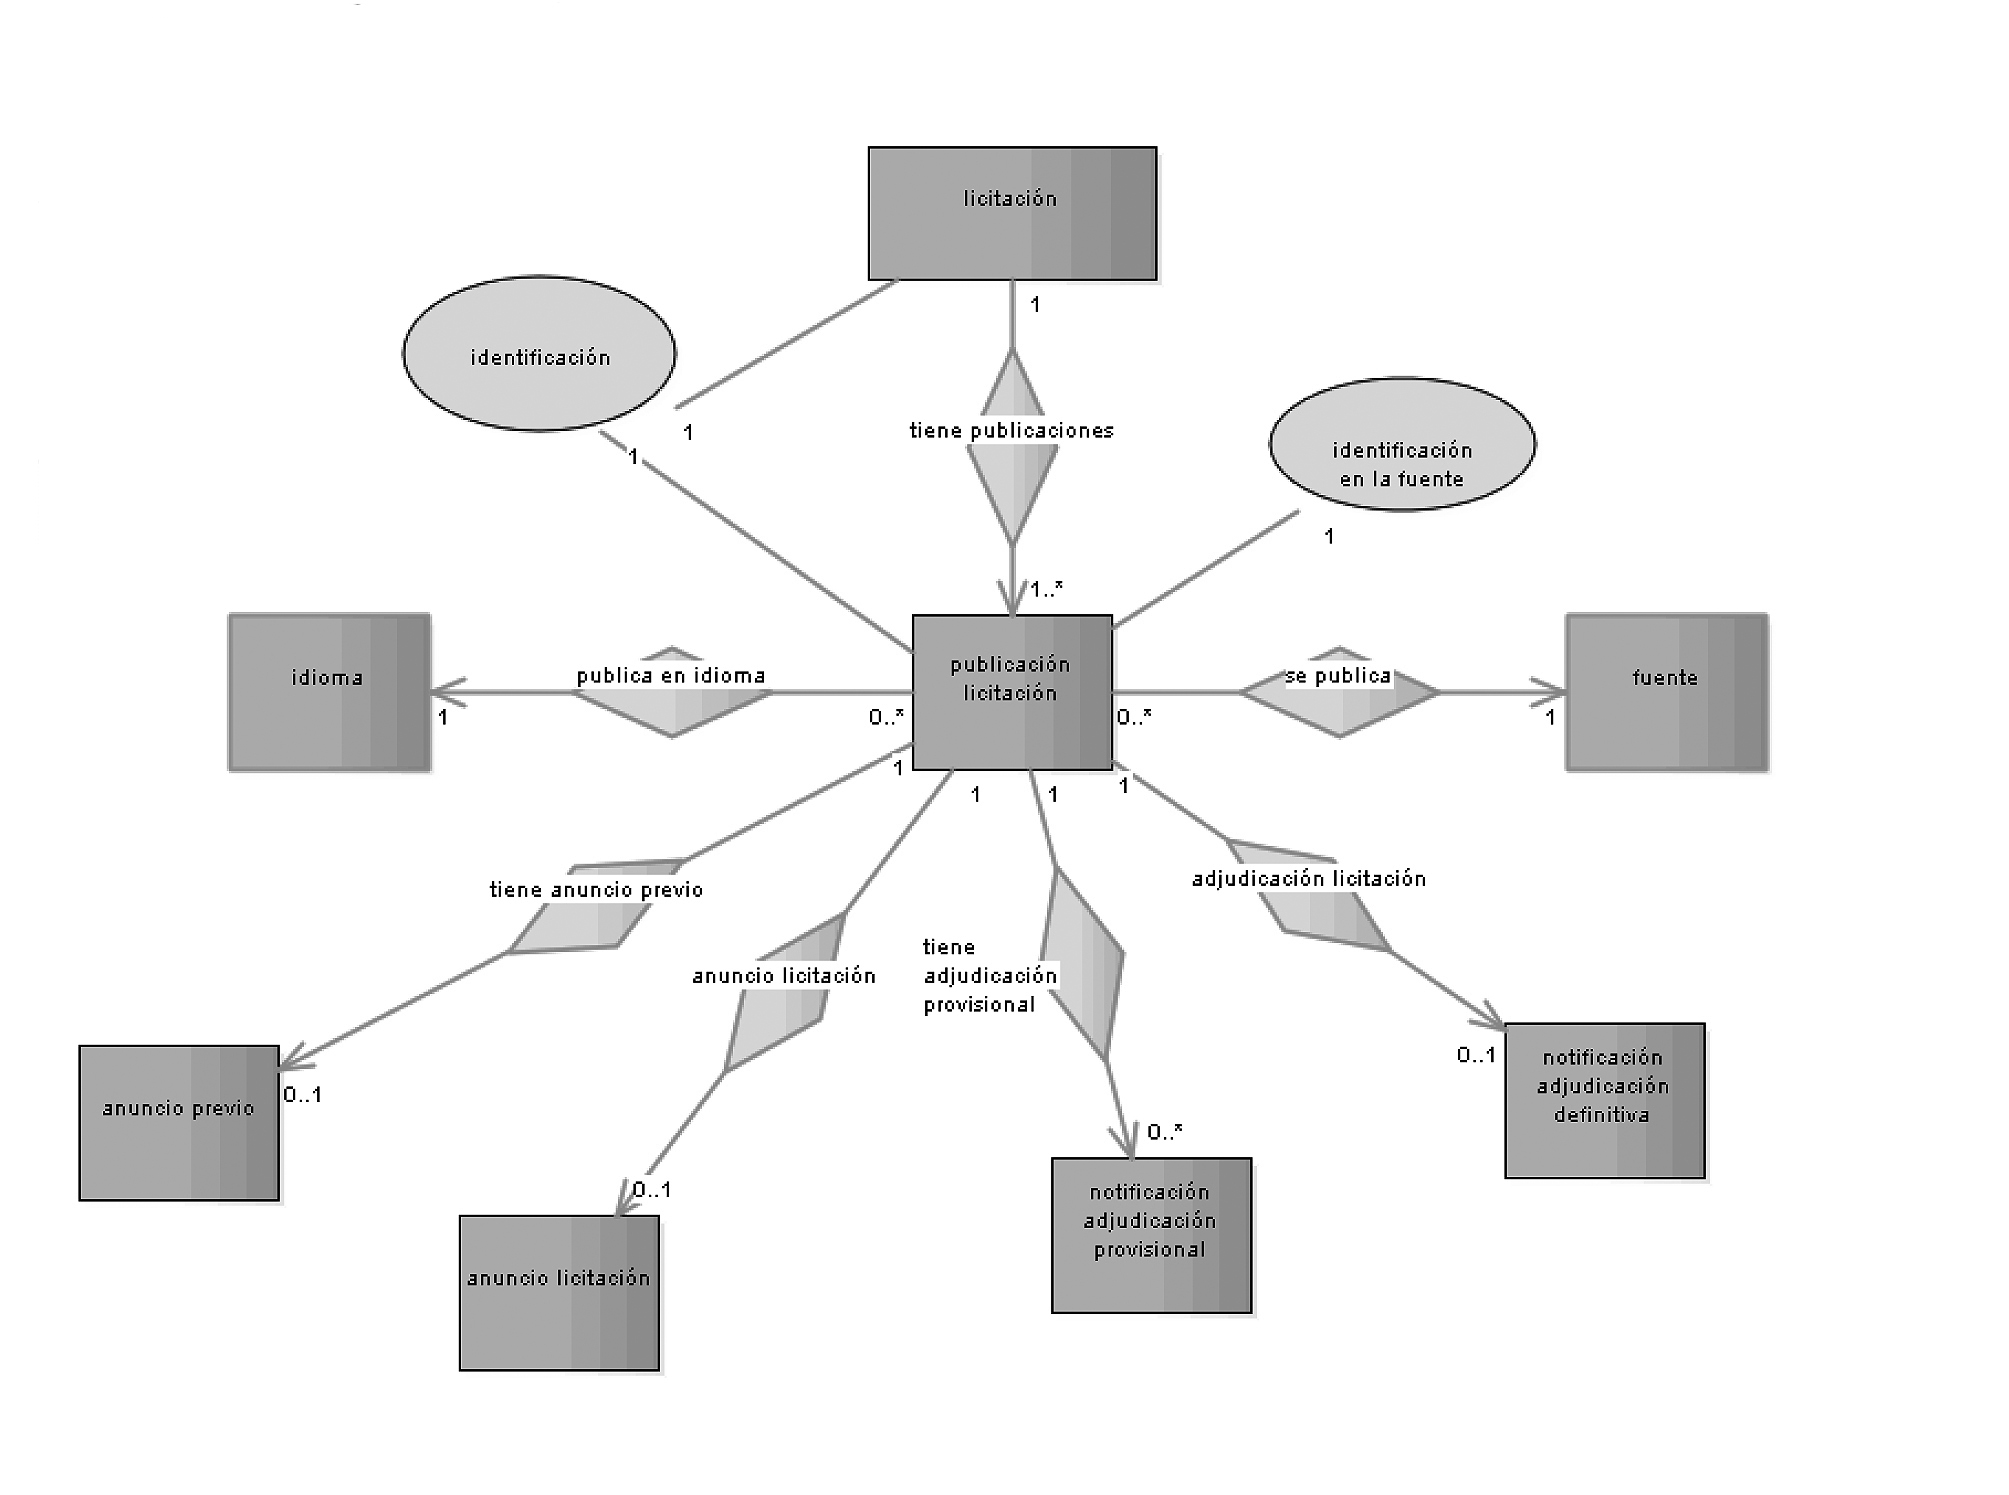
\includegraphics[width=10cm]{images/phd/eproc/10ders-1}
% \caption{Publicación de Anuncio de Licitación en el proyecto 10ders.}
% \label{fig:10ders-1}
% \end{figure}
% 
% 
% \begin{figure}[!htb]
% \centering
% 	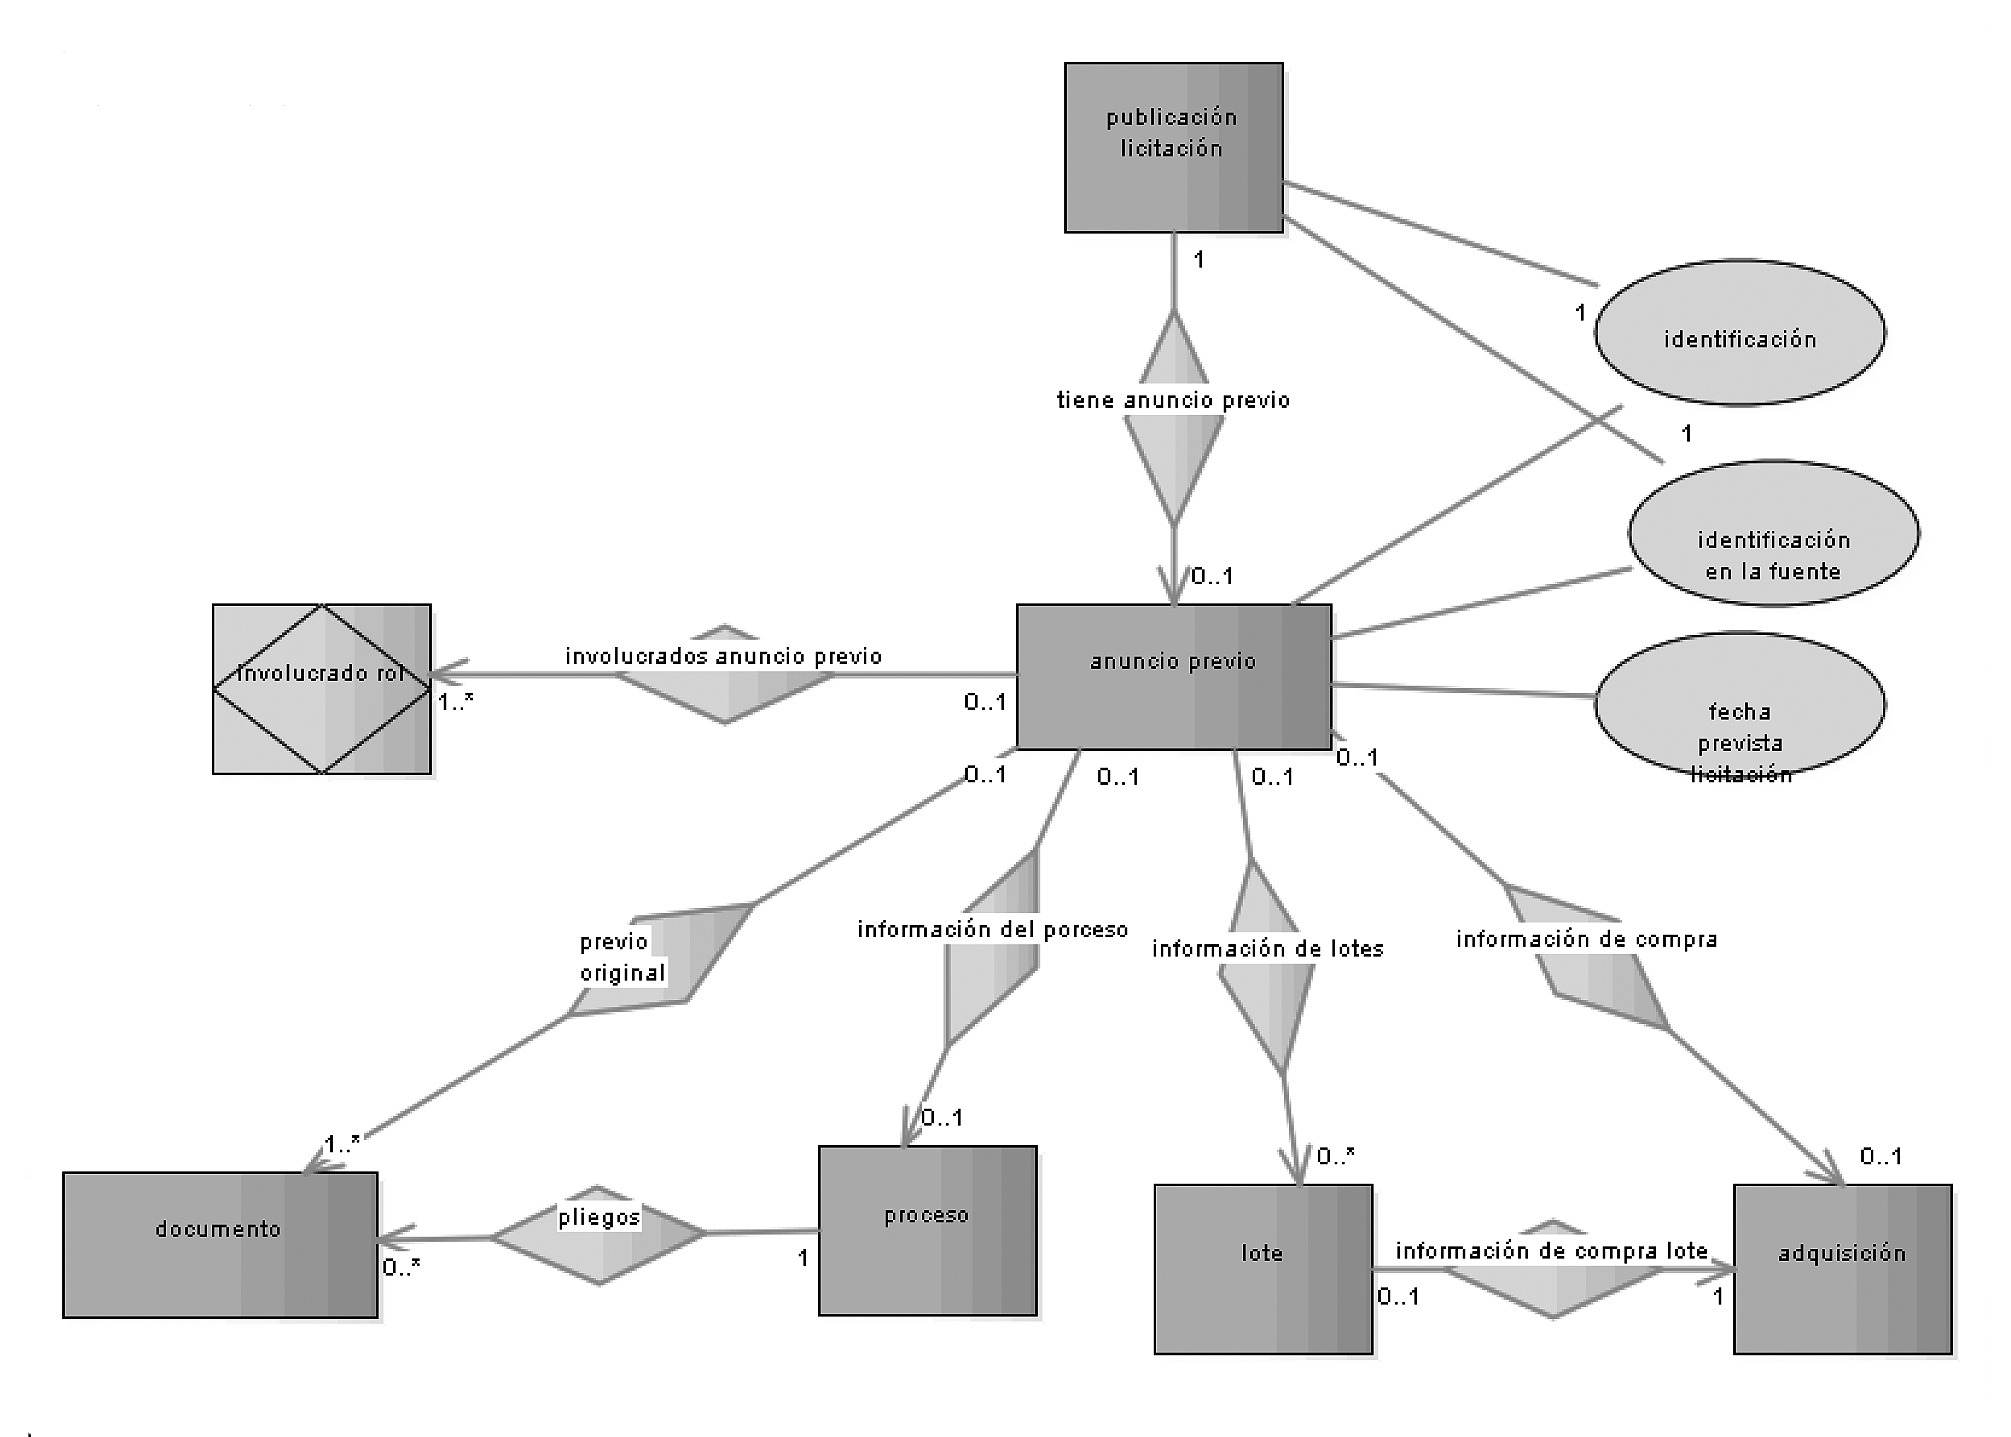
\includegraphics[width=10cm]{images/phd/eproc/10ders-2}
% \caption{Anuncio Previo de Licitación en el proyecto 10ders.}
% \label{fig:10ders-2}
% \end{figure}
% 
% 
% \begin{figure}[!htb]
% \centering
% 	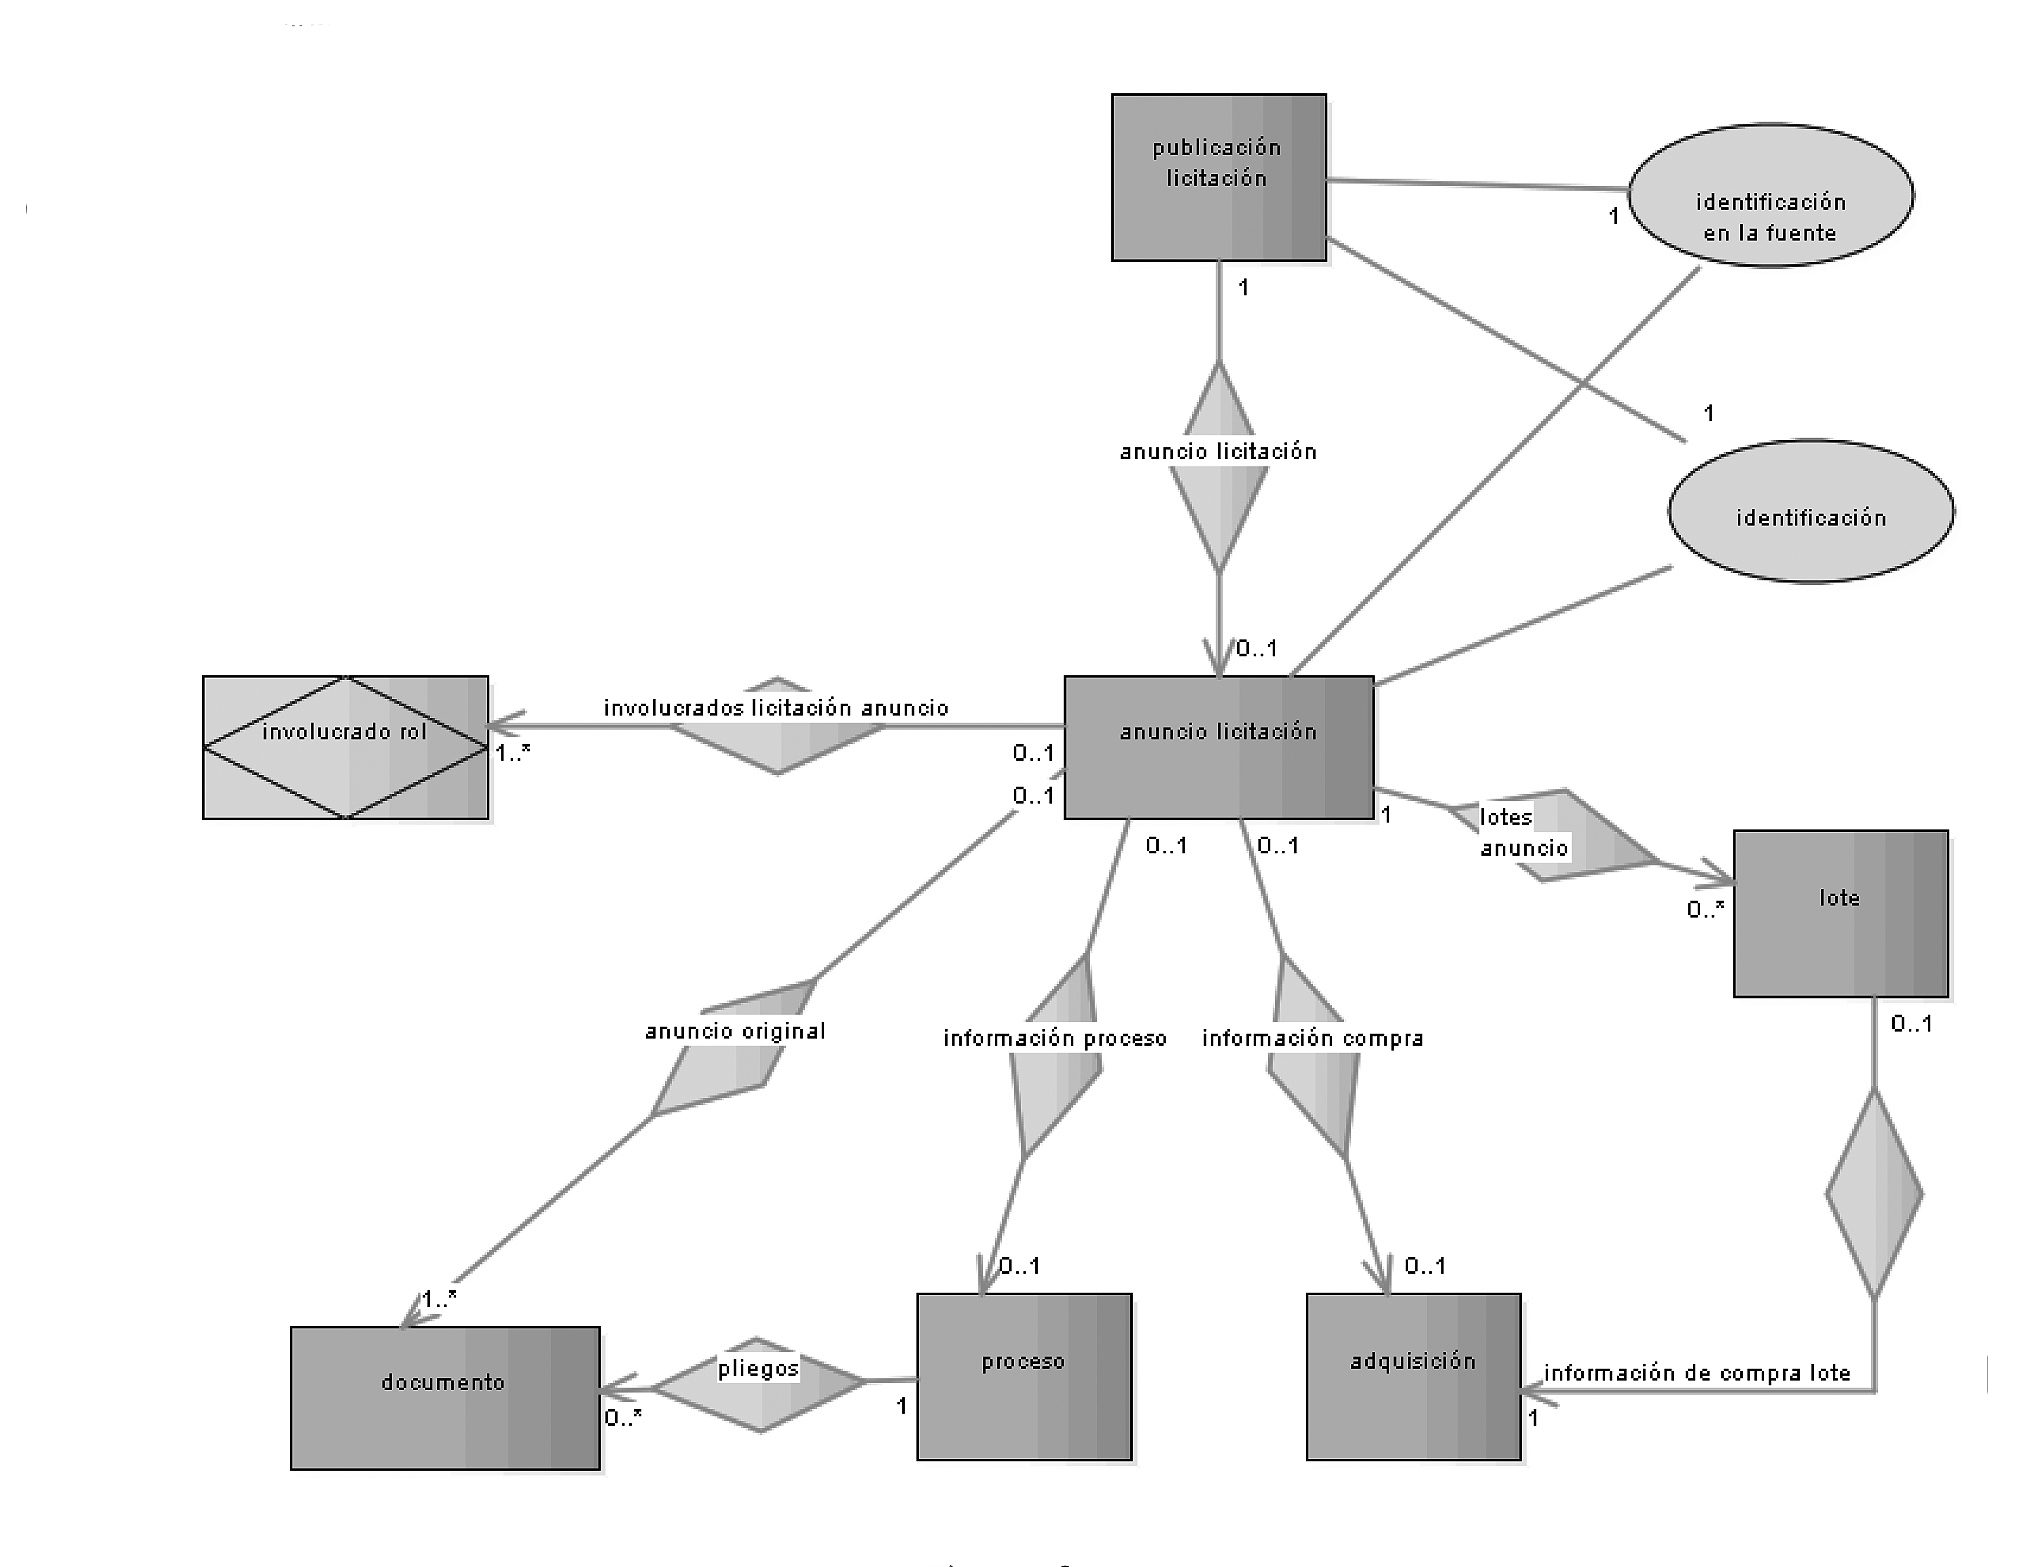
\includegraphics[width=10cm]{images/phd/eproc/10ders-3}
% \caption{Anuncio de Licitación en el proyecto 10ders.}
% \label{fig:10ders-3}
% \end{figure}
% 
% \begin{figure}[!htb]
% \centering
% 	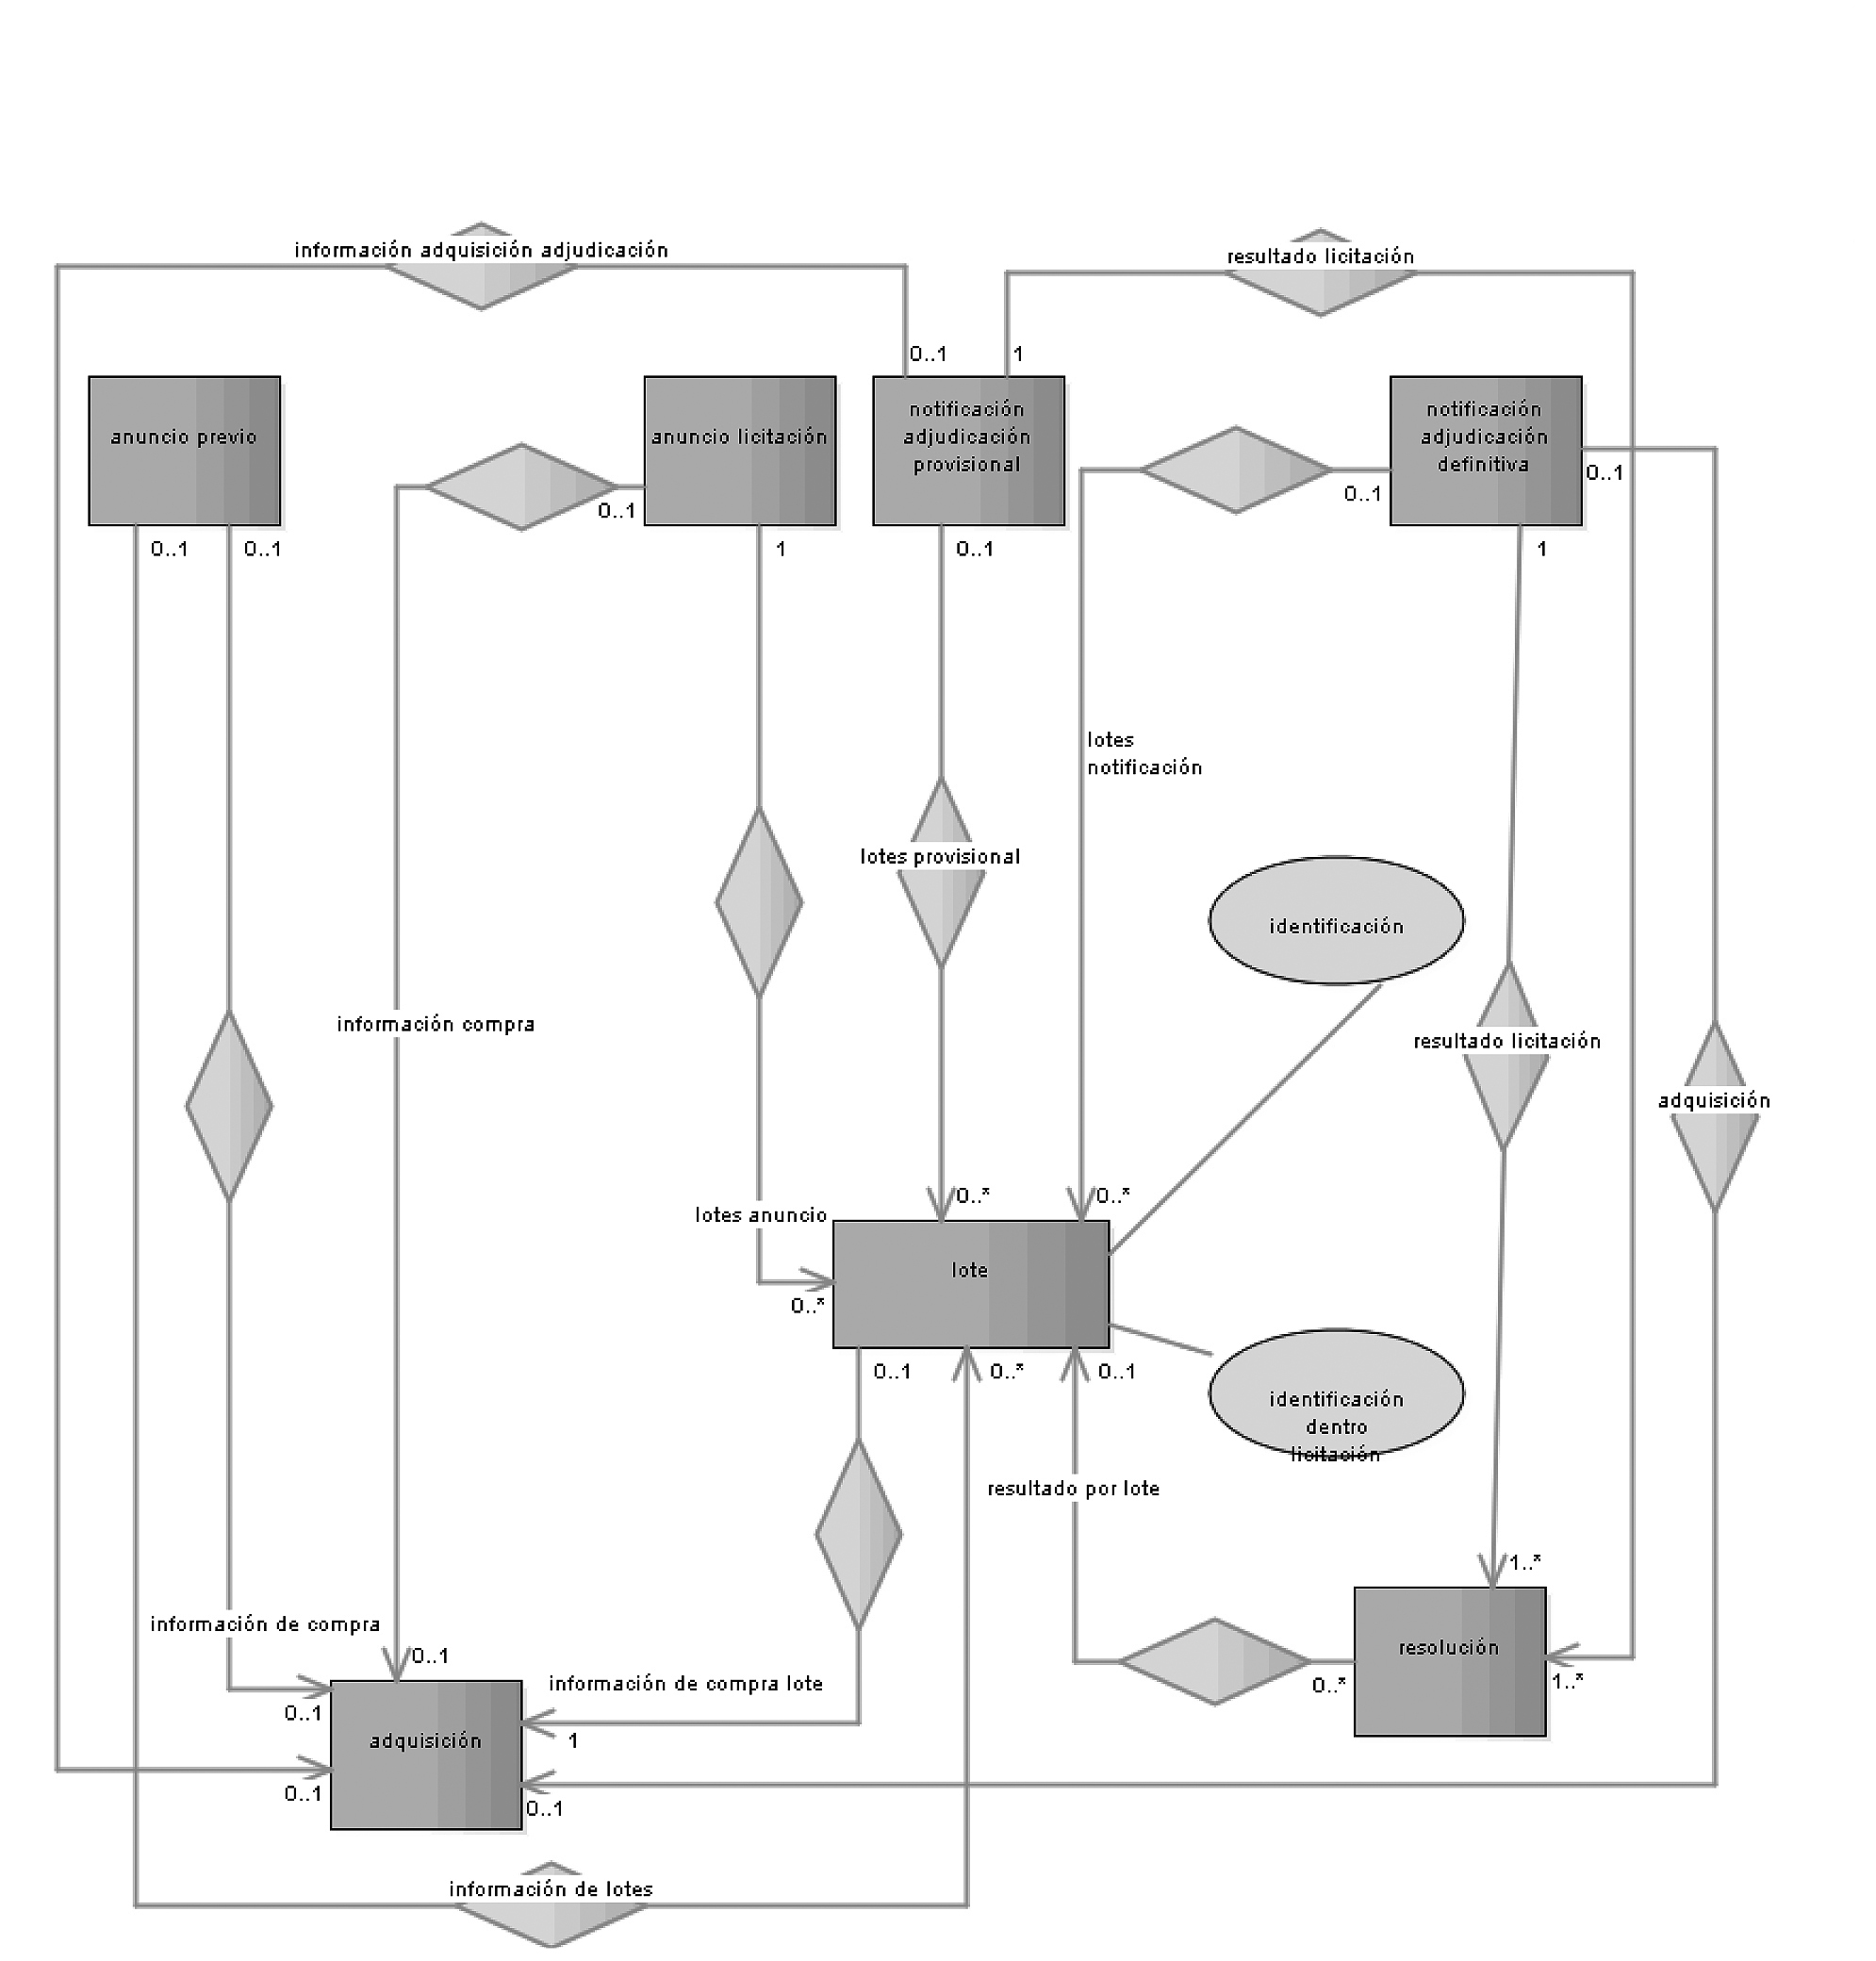
\includegraphics[width=10cm]{images/phd/eproc/10ders-6}
% \caption{Lote en el proyecto 10ders.}
% \label{fig:10ders-6}
% \end{figure}
% 
% 
% \begin{figure}[!htb]
% \centering
% 	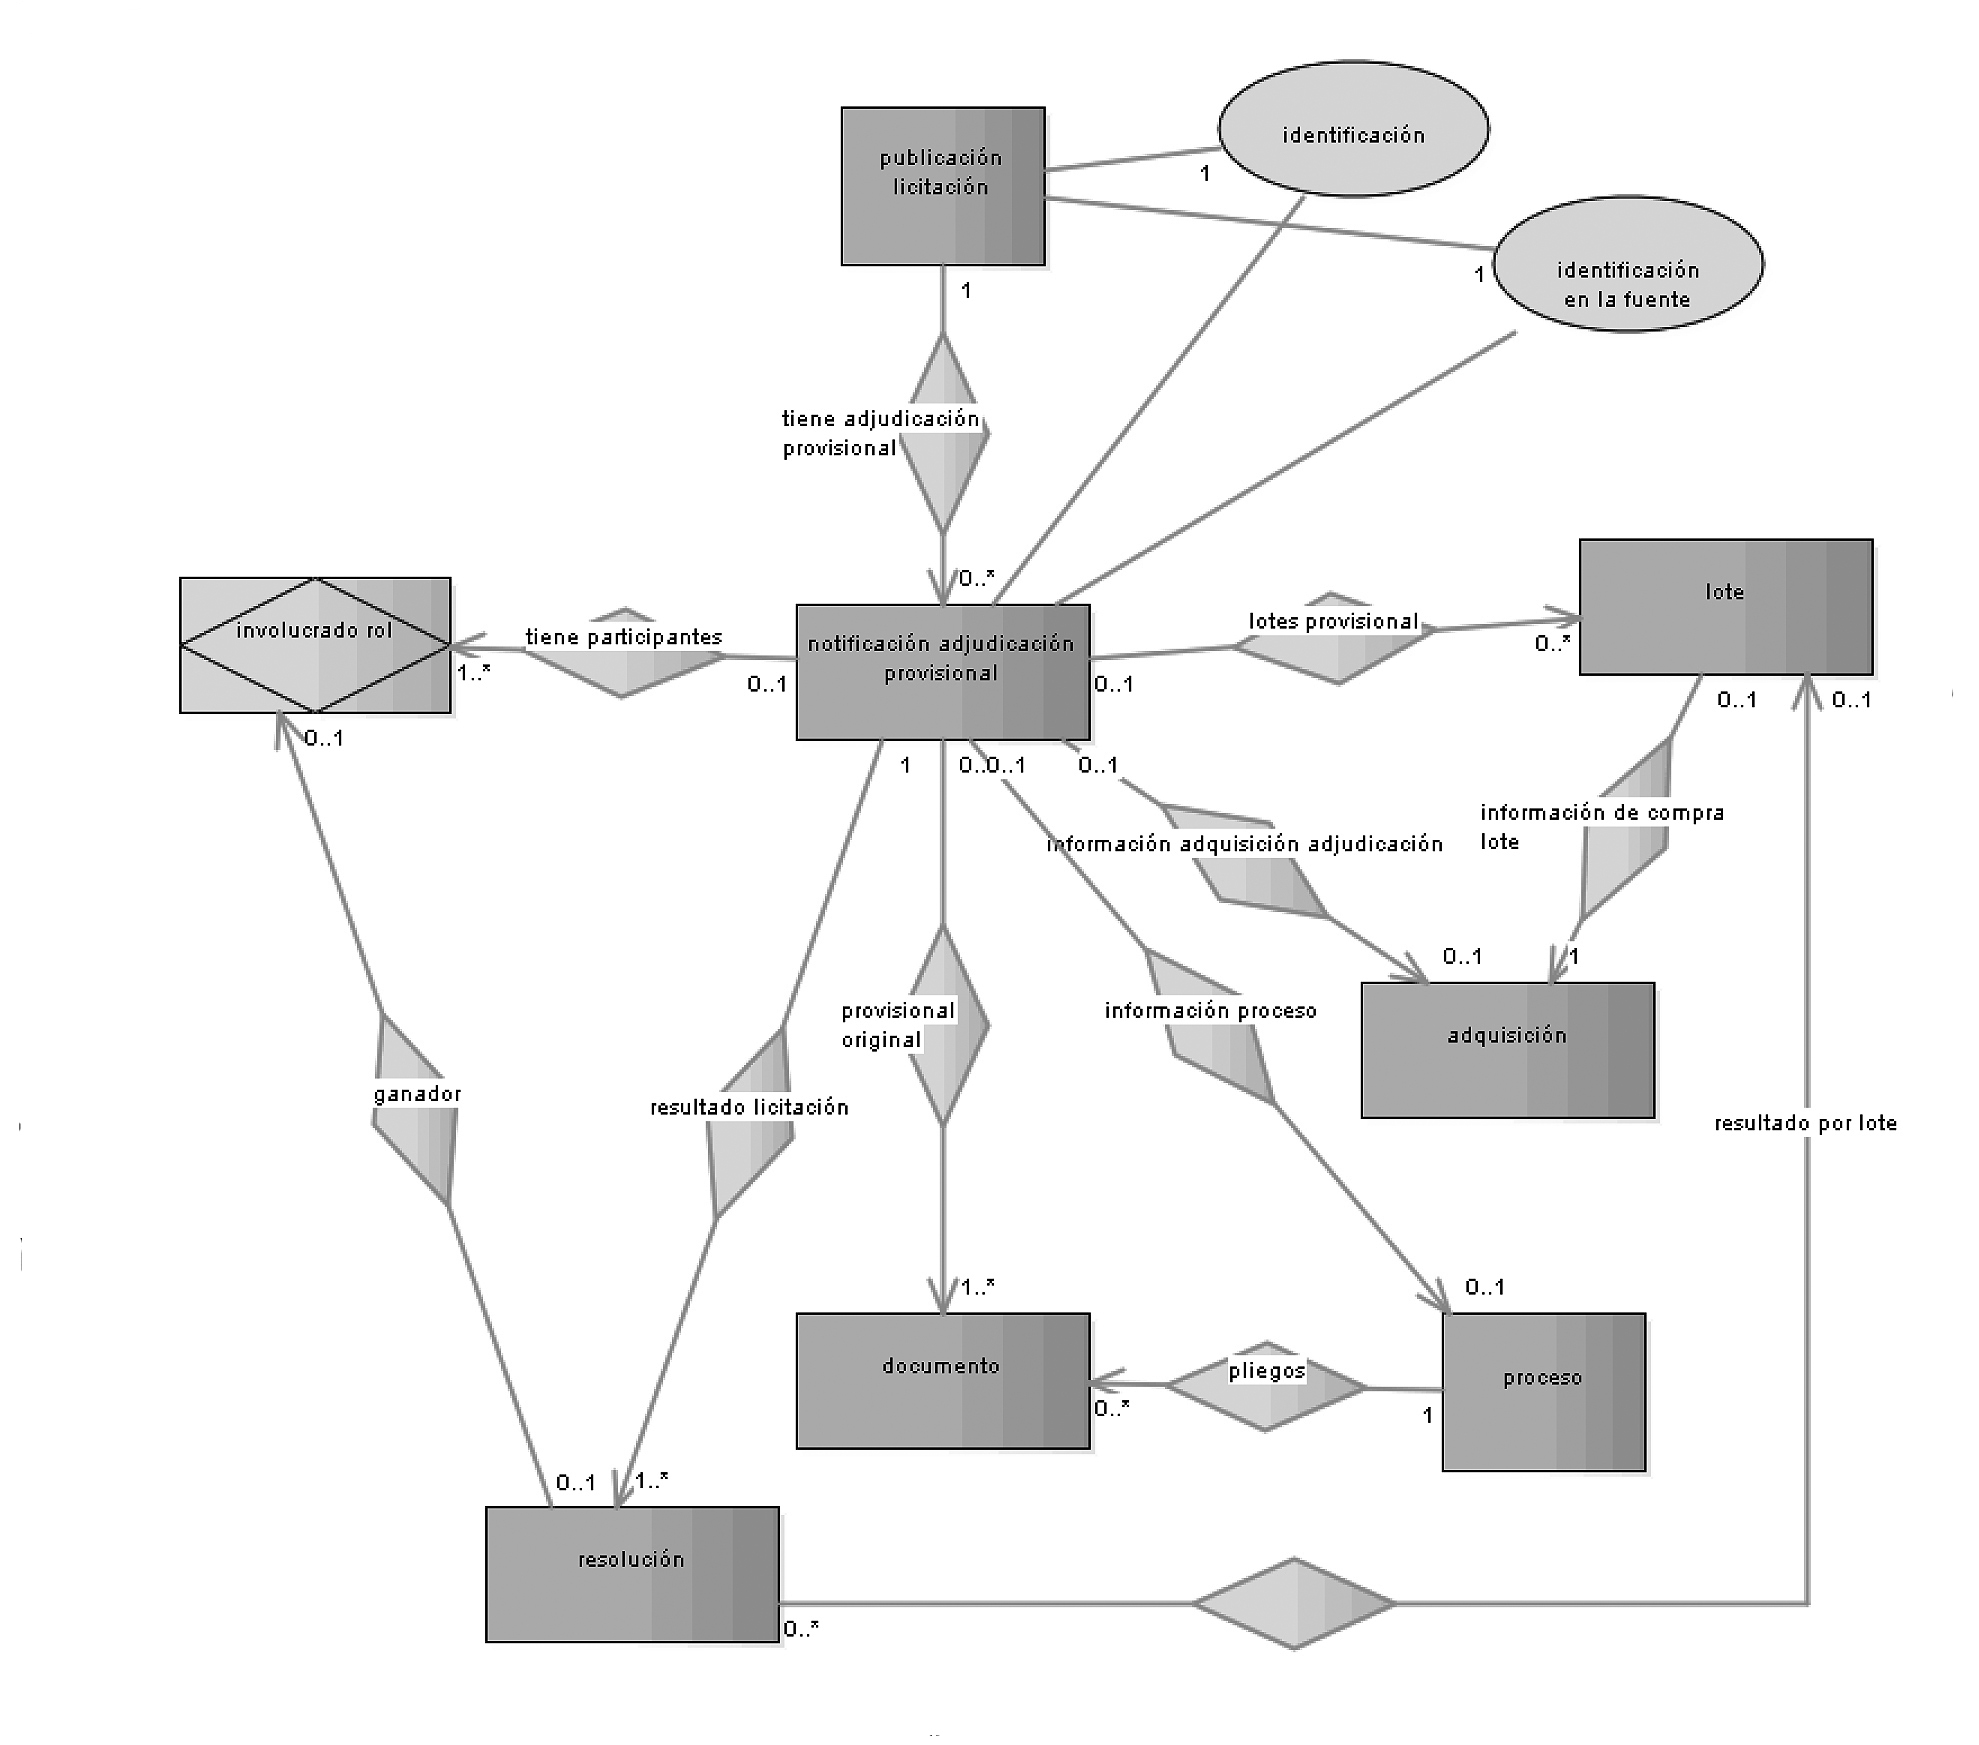
\includegraphics[width=10cm]{images/phd/eproc/10ders-4}
% \caption{Notificación de Adjudicación Provisional el proyecto 10ders.}
% \label{fig:10ders-4}
% \end{figure}
% 
% 
% 
% \begin{figure}[!htb]
% \centering
% 	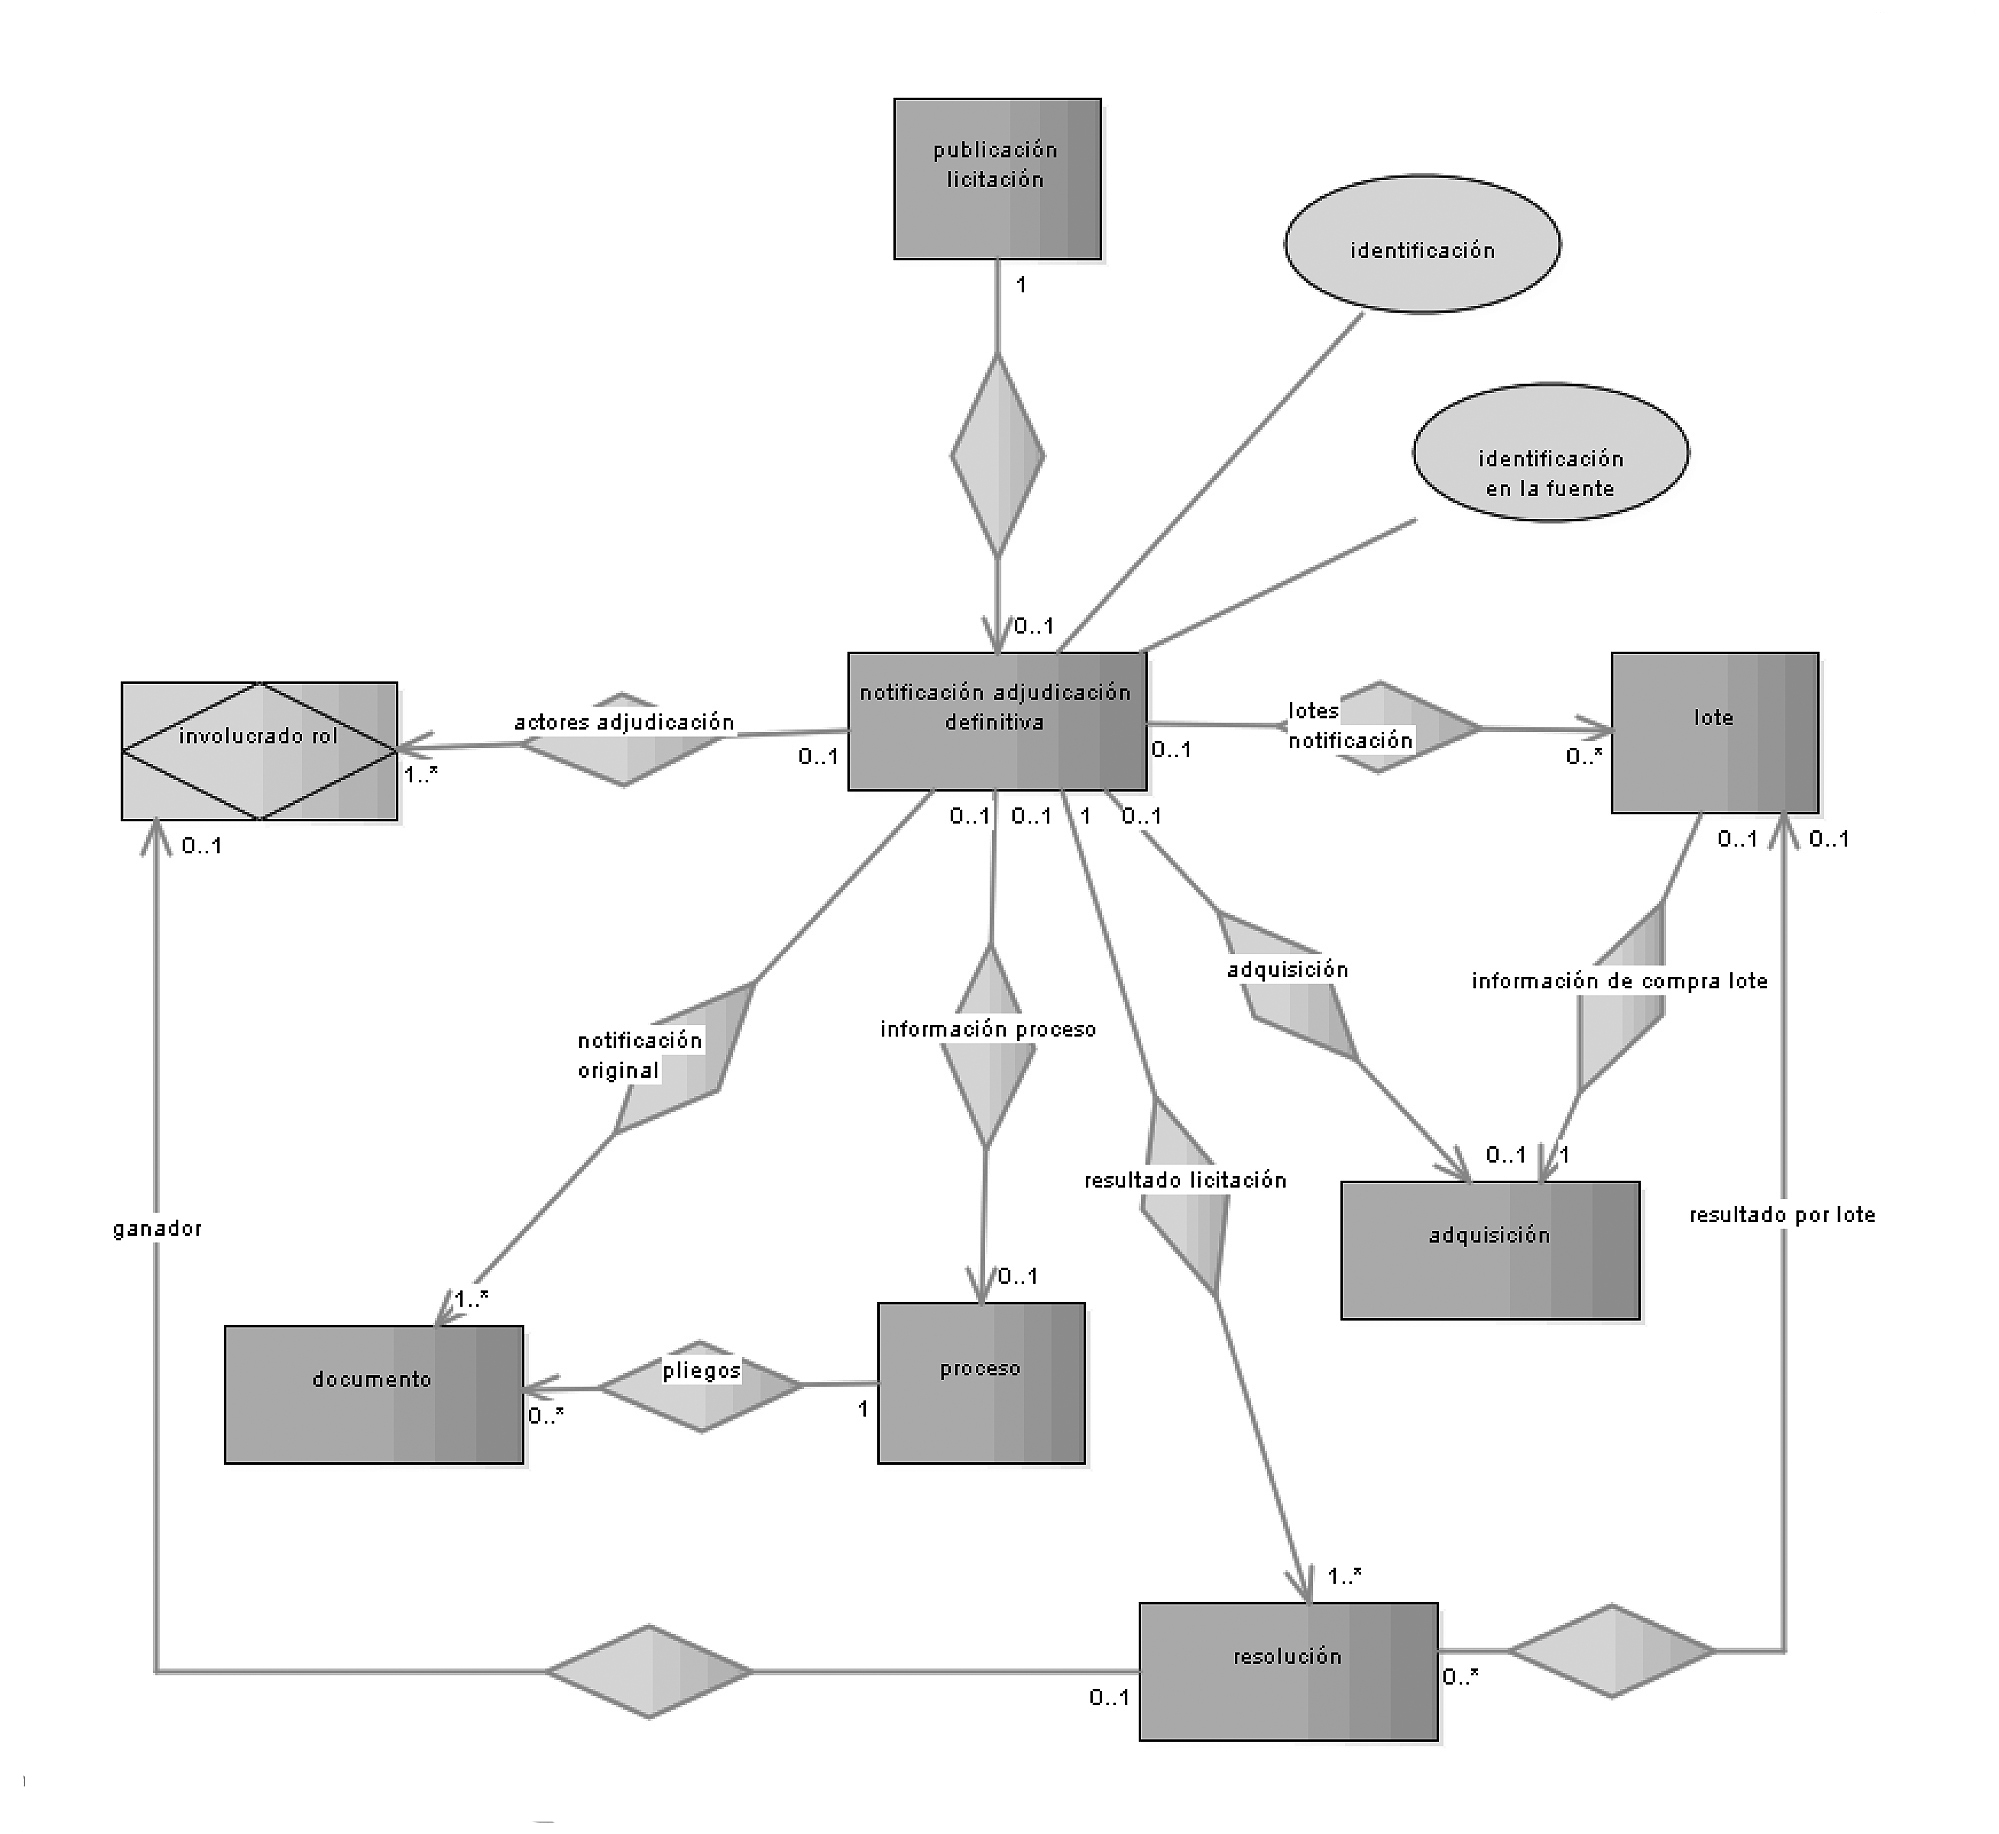
\includegraphics[width=10cm]{images/phd/eproc/10ders-5}
% \caption{Notificación de Adjudicación Definitiva el proyecto 10ders.}
% \label{fig:10ders-5}
% \end{figure}
% 
% 
% 
% \begin{figure}[!htb]
% \centering
% 	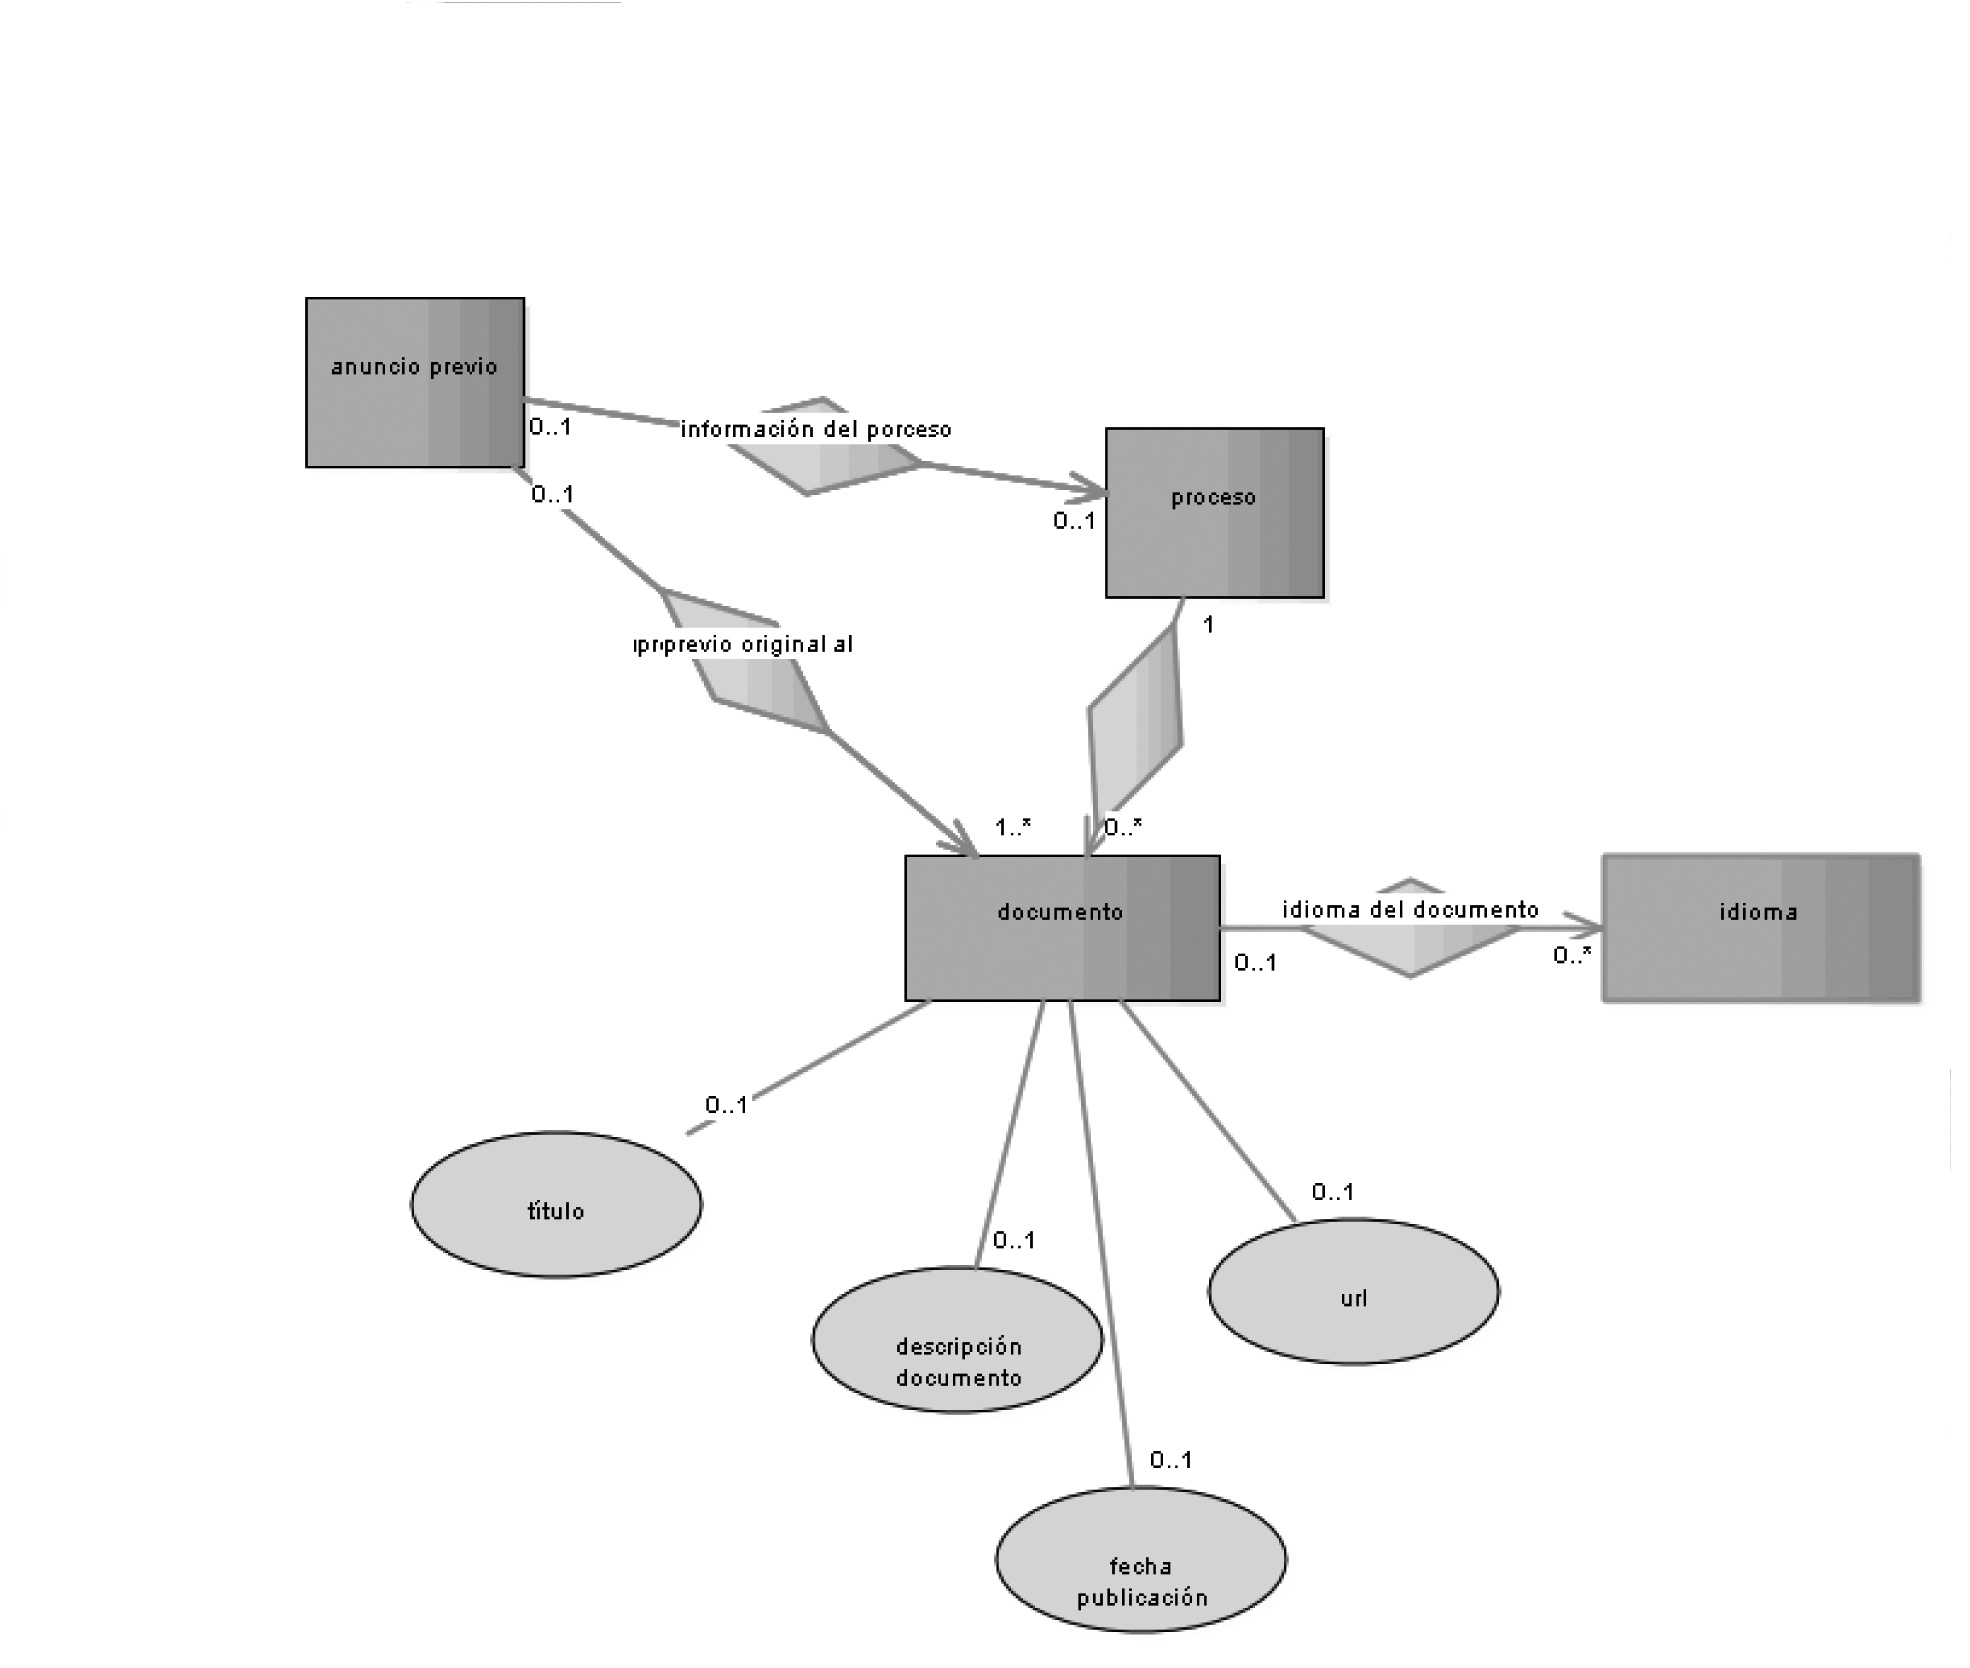
\includegraphics[width=10cm]{images/phd/eproc/10ders-7}
% \caption{Documento en el proyecto 10ders.}
% \label{fig:10ders-7}
% \end{figure}


% 


% 










